\chapter{Computer architecture}
\label{ch:arch}
\section{Electronics}

\begin{wrapfigure}{r}{0.3\textwidth}
    \centering
    \begin{tikzpicture}[
    >={Stealth[round]},
    inner xsep = 1em,
    minimum height = 2em,
]
    \node[circle, draw, minimum size = 4em] {};
    \draw[line width = 0.25em] (-0.125, -0.4) -- (-0.125, 0.4);
    \node (source) at (1.4142em, 1.75) {source};
    \node (drain) at (1.4142em, -1.75) {drain};
    \node (gate) at (-2, 0) {gate};
    \draw[->] (gate) -- (-0.125, 0);
    \draw[->] (source) -- (1.4142em, 1.4142em) -- (-0.125, 0.1);
    \draw[->] (-0.125, -0.1) -- (1.4142em, -1.4142em) -- (drain);
\end{tikzpicture}

    \caption{Transistor}
    \label{fig:arch:trans}
\end{wrapfigure}

The elemental component of digital circuits is the \textit{transistor}: a very
small semiconductor device which can be used to control electrical signals.
Transistors, as commonly used in circuits, have conceptually three
\textit{terminals}: \textit{source} and \textit{drain} (i.e. input/output) and a
\textit{gate} (figure \ref{fig:arch:trans})\footnotemark.  Whenever voltage is
applied to the gate, current is allowed to flow from the source to the drain.
In the absence of that voltage, no current flows through the conductor.  This
allows current to be applied selectively according to an input signal.  Multiple
transistors can be combined to create basic logic gates (figure
\ref{fig:arch:trans_gates}):

\footnotetext{
    Alternative names for these terminals are \textit{emitter},
    \textit{collector}, and \textit{base}, respectively.}

\begin{itemize}
    \item
        An \textit{and} gate is formed with two transistors whose signals are
        connected serially: current flows only if both inputs are enabled.
    \item
        An \textit{or} gate is formed with two transistors whose signals are
        connected in parallel: current flows when either of the inputs is
        enabled.
\end{itemize}

To simplify notation, these circuits are normally idealized in an abstract form.
A special symbol is used instead of the full circuit and only the transistor
gates and the output are shown, usually labeled \texttt{a}, \texttt{b}, and
\texttt{out}, respectivelly (figure \ref{fig:arch:gate_symbols}).

\begin{figure}[ht]
    \centering
    \begin{subfigure}{0.4\textwidth}
        \centering
        \begin{tikzpicture}[circuit_diagram]
            \node[and gate] (g) {};
            \node[left = 0.5 of g.input 1] (a) {\texttt{a}};
            \node[left = 0.5 of g.input 2] (b) {\texttt{b}};
            \node[right = 0.5 of g.output] (out) {out};
            \draw (g.input 1) -- (a);
            \draw (g.input 2) -- (b);
            \draw (g.output) -- (out);
        \end{tikzpicture}
        \caption{\textit{and} gate}
    \end{subfigure}
    \begin{subfigure}{0.4\textwidth}
        \centering
        \begin{tikzpicture}[circuit_diagram]
            \node[or gate] (g) {};
            \node[left = 0.5 of g.input 1] (a) {\texttt{a}};
            \node[left = 0.5 of g.input 2] (b) {\texttt{b}};
            \node[right = 0.5 of g.output] (out) {\texttt{out}};
            \draw (g.input 1) -- (a);
            \draw (g.input 2) -- (b);
            \draw (g.output) -- (out);
        \end{tikzpicture}
        \caption{\textit{or} gate}
    \end{subfigure}
    \caption{Logic gate symbols}
    \label{fig:arch:gate_symbols}
\end{figure}

\begin{figure}[p]
    \centering
    \begin{subfigure}{\textwidth}
        \centering
        \begin{subfigure}{0.225\textwidth}
            \begin{tikzpicture}[
    >={Stealth[round]},
    inner xsep = 1em,
    minimum height = 2em,
]
    \begin{scope}[yshift = 4em]
        \node[circle, draw, minimum size = 4em] {};
        \draw[line width = 0.25em] (-0.125, -0.4) -- (-0.125, 0.4);
        \node (source0) at (1.4142em, 1.75) {};
        \node[minimum size = 0pt, inner sep = 0pt]
            (drain0) at (1.4142em, -1.75) {};
        \node (gate0) at (-2, 0) {};
        \draw[->] (gate0) -- (-0.125, 0);
        \draw[->, red, thick]
            (source0) -- (1.4142em, 1.4142em) -- (-0.125, 0.1);
        \draw[->] (-0.125, -0.1) -- (1.4142em, -1.4142em) -- (drain0);
    \end{scope}
    \begin{scope}[yshift = -4em]
        \node[circle, draw, minimum size = 4em] {};
        \draw[line width = 0.25em] (-0.125, -0.4) -- (-0.125, 0.4);
        \node (source1) at (1.4142em, 1.75) {};
        \node[minimum size = 0pt, inner sep = 0pt]
            (drain1) at (1.4142em, -1.75) {};
        \node (gate1) at (-2, 0) {};
        \draw[->] (gate1) -- (-0.125, 0);
        \draw[->] (source1) -- (1.4142em, 1.4142em) -- (-0.125, 0.1);
        \draw[->] (-0.125, -0.1) -- (1.4142em, -1.4142em) -- (drain1);
    \end{scope}
\end{tikzpicture}

        \end{subfigure}
        \begin{subfigure}{0.225\textwidth}
            \begin{tikzpicture}[
    >={Stealth[round]},
    inner xsep = 1em,
    minimum height = 2em,
]
    \begin{scope}[yshift = 4em]
        \node[circle, draw, minimum size = 4em] {};
        \draw[line width = 0.25em] (-0.125, -0.4) -- (-0.125, 0.4);
        \node (source0) at (1.4142em, 1.75) {};
        \node[minimum size = 0pt, inner sep = 0pt]
            (drain0) at (1.4142em, -1.75) {};
        \node (gate0) at (-2, 0) {};
        \draw[->, red, thick] (gate0) -- (-0.125, 0);
        \draw[->, red, thick]
            (source0) -- (1.4142em, 1.4142em) -- (-0.125, 0.1);
        \draw[->, red, thick]
            (-0.125, -0.1) -- (1.4142em, -1.4142em) -- (drain0);
    \end{scope}
    \begin{scope}[yshift = -4em]
        \node[circle, draw, minimum size = 4em] {};
        \draw[line width = 0.25em] (-0.125, -0.4) -- (-0.125, 0.4);
        \node (source1) at (1.4142em, 1.75) {};
        \node[minimum size = 0pt, inner sep = 0pt]
            (drain1) at (1.4142em, -1.75) {};
        \node (gate1) at (-2, 0) {};
        \draw[->] (gate1) -- (-0.125, 0);
        \draw[->, red, thick]
            (source1) -- (1.4142em, 1.4142em) -- (-0.125, 0.1);
        \draw[->] (-0.125, -0.1) -- (1.4142em, -1.4142em) -- (drain1);
    \end{scope}
\end{tikzpicture}

        \end{subfigure}
        \begin{subfigure}{0.225\textwidth}
            \begin{tikzpicture}[
    >={Stealth[round]},
    inner xsep = 1em,
    minimum height = 2em,
]
    \begin{scope}[yshift = 4em]
        \node[circle, draw, minimum size = 4em] {};
        \draw[line width = 0.25em] (-0.125, -0.4) -- (-0.125, 0.4);
        \node (source0) at (1.4142em, 1.75) {};
        \node[minimum size = 0pt, inner sep = 0pt]
            (drain0) at (1.4142em, -1.75) {};
        \node (gate0) at (-2, 0) {};
        \draw[->] (gate0) -- (-0.125, 0);
        \draw[->, red, thick]
            (source0) -- (1.4142em, 1.4142em) -- (-0.125, 0.1);
        \draw[->] (-0.125, -0.1) -- (1.4142em, -1.4142em) -- (drain0);
    \end{scope}
    \begin{scope}[yshift = -4em]
        \node[circle, draw, minimum size = 4em] {};
        \draw[line width = 0.25em] (-0.125, -0.4) -- (-0.125, 0.4);
        \node (source1) at (1.4142em, 1.75) {};
        \node[minimum size = 0pt, inner sep = 0pt]
            (drain1) at (1.4142em, -1.75) {};
        \node (gate1) at (-2, 0) {};
        \draw[->, red, thick] (gate1) -- (-0.125, 0);
        \draw[->] (source1) -- (1.4142em, 1.4142em) -- (-0.125, 0.1);
        \draw[->] (-0.125, -0.1) -- (1.4142em, -1.4142em) -- (drain1);
    \end{scope}
\end{tikzpicture}

        \end{subfigure}
        \begin{subfigure}{0.225\textwidth}
            \begin{tikzpicture}[
    >={Stealth[round]},
    inner xsep = 1em,
    minimum height = 2em,
]
    \begin{scope}[yshift = 4em]
        \node[circle, draw, minimum size = 4em] {};
        \draw[line width = 0.25em] (-0.125, -0.4) -- (-0.125, 0.4);
        \node (source0) at (1.4142em, 1.75) {};
        \node[minimum size = 0pt, inner sep = 0pt]
            (drain0) at (1.4142em, -1.75) {};
        \node (gate0) at (-2, 0) {};
        \draw[->, red, thick] (gate0) -- (-0.125, 0);
        \draw[->, red, thick]
            (source0) -- (1.4142em, 1.4142em) -- (-0.125, 0.1);
        \draw[->, red, thick]
            (-0.125, -0.1) -- (1.4142em, -1.4142em) -- (drain0);
    \end{scope}
    \begin{scope}[yshift = -4em]
        \node[circle, draw, minimum size = 4em] {};
        \draw[line width = 0.25em] (-0.125, -0.4) -- (-0.125, 0.4);
        \node (source1) at (1.4142em, 1.75) {};
        \node[minimum size = 0pt, inner sep = 0pt]
            (drain1) at (1.4142em, -1.75) {};
        \node (gate1) at (-2, 0) {};
        \draw[->, red, thick] (gate1) -- (-0.125, 0);
        \draw[->, red, thick]
            (source1) -- (1.4142em, 1.4142em) -- (-0.125, 0.1);
        \draw[->, red, thick]
            (-0.125, -0.1) -- (1.4142em, -1.4142em) -- (drain1);
    \end{scope}
\end{tikzpicture}

        \end{subfigure}
        \\[2em]
        \caption{\textit{and} gate}
    \end{subfigure}
    \\[2em]
    \begin{subfigure}{\textwidth}
        \centering
        \begin{subfigure}{0.4\textwidth}
            \begin{tikzpicture}[
    >={Stealth[round]},
    inner xsep = 1em,
    minimum height = 2em,
]
    \node[inner sep = 0pt, minimum size = 0pt] (source) at (0.5, 2) {};
    \node[inner sep = 0pt, minimum size = 0pt] (drain) at (0.5, -1.5) {};
    \begin{scope}[xshift = -3em]
        \node[circle, draw, minimum size = 4em] {};
        \draw[line width = 0.25em] (-0.125, -0.4) -- (-0.125, 0.4);
        \node[inner sep = 0pt, minimum size = 0pt]
            (source0) at (1.4142em, 1.5) {};
        \node (gate0) at (-1.5, 0) {};
        \draw[->] (gate0) -- (-0.125, 0);
        \draw[->, red, thick]
            (source) |- (source0) -- (1.4142em, 1.4142em) -- (-0.125, 0.1);
        \draw (-0.125, -0.1) -- (1.4142em, -1.4142em) |- (drain);
    \end{scope}
    \begin{scope}[xshift = 3em]
        \node[circle, draw, minimum size = 4em] {};
        \draw[line width = 0.25em] (-0.125, -0.4) -- (-0.125, 0.4);
        \node[inner sep = 0pt, minimum size = 0pt]
            (source1) at (1.4142em, 1.5) {};
        \node (gate1) at (-1.5, 0) {};
        \draw[->] (gate1) -- (-0.125, 0);
        \draw[->, red, thick]
            (source) |- (source1) -- (1.4142em, 1.4142em) -- (-0.125, 0.1);
        \draw (-0.125, -0.1) -- (1.4142em, -1.4142em) |- (drain);
    \end{scope}
    \draw[->] (drain) -- +(0, -0.5);
\end{tikzpicture}

        \end{subfigure}
        \begin{subfigure}{0.4\textwidth}
            \begin{tikzpicture}[
    >={Stealth[round]},
    inner xsep = 1em,
    minimum height = 2em,
]
    \node[inner sep = 0pt, minimum size = 0pt] (source) at (0.5, 2) {};
    \node[inner sep = 0pt, minimum size = 0pt] (drain) at (0.5, -1.5) {};
    \begin{scope}[xshift = -3em]
        \node[circle, draw, minimum size = 4em] {};
        \draw[line width = 0.25em] (-0.125, -0.4) -- (-0.125, 0.4);
        \node[inner sep = 0pt, minimum size = 0pt]
            (source0) at (1.4142em, 1.5) {};
        \node (gate0) at (-1.5, 0) {};
        \draw[->, red, thick] (gate0) -- (-0.125, 0);
        \draw[->, red, thick]
            (source) |- (source0) -- (1.4142em, 1.4142em) -- (-0.125, 0.1);
        \draw[red, thick] (-0.125, -0.1) -- (1.4142em, -1.4142em) |- (drain);
    \end{scope}
    \begin{scope}[xshift = 3em]
        \node[circle, draw, minimum size = 4em] {};
        \draw[line width = 0.25em] (-0.125, -0.4) -- (-0.125, 0.4);
        \node[inner sep = 0pt, minimum size = 0pt]
            (source1) at (1.4142em, 1.5) {};
        \node (gate1) at (-1.5, 0) {};
        \draw[->] (gate1) -- (-0.125, 0);
        \draw[->, red, thick]
            (source) |- (source1) -- (1.4142em, 1.4142em) -- (-0.125, 0.1);
        \draw (-0.125, -0.1) -- (1.4142em, -1.4142em) |- (drain);
    \end{scope}
    \draw[->, red, thick] (drain) -- +(0, -0.5);
\end{tikzpicture}

        \end{subfigure}
        \\~\\
        \begin{subfigure}{0.4\textwidth}
            \begin{tikzpicture}[
    >={Stealth[round]},
    inner xsep = 1em,
    minimum height = 2em,
]
    \node[inner sep = 0pt, minimum size = 0pt] (source) at (0.5, 2) {};
    \node[inner sep = 0pt, minimum size = 0pt] (drain) at (0.5, -1.5) {};
    \begin{scope}[xshift = -3em]
        \node[circle, draw, minimum size = 4em] {};
        \draw[line width = 0.25em] (-0.125, -0.4) -- (-0.125, 0.4);
        \node[inner sep = 0pt, minimum size = 0pt]
            (source0) at (1.4142em, 1.5) {};
        \node (gate0) at (-1.5, 0) {};
        \draw[->] (gate0) -- (-0.125, 0);
        \draw[->, red, thick]
            (source) |- (source0) -- (1.4142em, 1.4142em) -- (-0.125, 0.1);
        \draw (-0.125, -0.1) -- (1.4142em, -1.4142em) |- (drain);
    \end{scope}
    \begin{scope}[xshift = 3em]
        \node[circle, draw, minimum size = 4em] {};
        \draw[line width = 0.25em] (-0.125, -0.4) -- (-0.125, 0.4);
        \node[inner sep = 0pt, minimum size = 0pt]
            (source1) at (1.4142em, 1.5) {};
        \node (gate1) at (-1.5, 0) {};
        \draw[->, red, thick] (gate1) -- (-0.125, 0);
        \draw[->, red, thick]
            (source) |- (source1) -- (1.4142em, 1.4142em) -- (-0.125, 0.1);
        \draw[red, thick] (-0.125, -0.1) -- (1.4142em, -1.4142em) |- (drain);
    \end{scope}
    \draw[->, red, thick] (drain) -- +(0, -0.5);
\end{tikzpicture}

        \end{subfigure}
        \begin{subfigure}{0.4\textwidth}
            \begin{tikzpicture}[
    >={Stealth[round]},
    inner xsep = 1em,
    minimum height = 2em,
]
    \node[inner sep = 0pt, minimum size = 0pt] (source) at (0.5, 2) {};
    \node[inner sep = 0pt, minimum size = 0pt] (drain) at (0.5, -1.5) {};
    \begin{scope}[xshift = -3em]
        \node[circle, draw, minimum size = 4em] {};
        \draw[line width = 0.25em] (-0.125, -0.4) -- (-0.125, 0.4);
        \node[inner sep = 0pt, minimum size = 0pt]
            (source0) at (1.4142em, 1.5) {};
        \node (gate0) at (-1.5, 0) {};
        \draw[->, red, thick] (gate0) -- (-0.125, 0);
        \draw[->, red, thick]
            (source) |- (source0) -- (1.4142em, 1.4142em) -- (-0.125, 0.1);
        \draw[red, thick] (-0.125, -0.1) -- (1.4142em, -1.4142em) |- (drain);
    \end{scope}
    \begin{scope}[xshift = 3em]
        \node[circle, draw, minimum size = 4em] {};
        \draw[line width = 0.25em] (-0.125, -0.4) -- (-0.125, 0.4);
        \node[inner sep = 0pt, minimum size = 0pt]
            (source1) at (1.4142em, 1.5) {};
        \node (gate1) at (-1.5, 0) {};
        \draw[->, red, thick] (gate1) -- (-0.125, 0);
        \draw[->, red, thick]
            (source) |- (source1) -- (1.4142em, 1.4142em) -- (-0.125, 0.1);
        \draw[red, thick] (-0.125, -0.1) -- (1.4142em, -1.4142em) |- (drain);
    \end{scope}
    \draw[->, red, thick] (drain) -- +(0, -0.5);
\end{tikzpicture}

        \end{subfigure}
        \\[1em]
        \caption{\textit{or} gate}
    \end{subfigure}
    \caption{Logic gates}
    \label{fig:arch:trans_gates}
\end{figure}

\section{Integers}

\label{sec:arch:int}

\subsection{Binary numbers and modular arithmetic}

\label{subsec:arch:bin}

Computers must operate on finite values.  This fact limits the maximum values of
numbers they can represent and manipulate.  The \textit{word size}\footnotemark
of a computer architecture determines the natural unit of data of the
instruction set and limits the size of numbers directly accessible.  Early
computers had 8-bit words and several word sizes have existed throughout
history, but common sizes are now 32 and 64 bits.

\footnotetext{
    Used here \textit{stricto sensu}, in contrast to the alternative definition
    of ``word'' as the word size of a particular ancestor of the architecture
    that is now maintained for backwards compatibility (e.g.  ``16-bit word'' in
    x86).}

A binary number with $n$ bits, or \textit{binary digits}, has $2^n$ possible
values.  Table \ref{tbl:arch:integers:bits} shows the common word sizes and the
number of integer values they can represent.  An 8-bit byte can represent two
hundred and fifty six distinct values, while that number is approximately sixty
five thousand, four billion, and eighteen quintillion for 16-, 32-, and 64-bit
numbers, respectively\footnotemark.

\footnotetext{
    Note that the progression of powers in radix 2 whose exponents are multiples
    of 10 is close to those in radix 10 whose exponents are multiples of 3,
    thus:
    \begin{alignat*}{11}
        2^{10} &\approx 10^3    & \quad & \delta\; &= 0.0234375 & \qquad &
        2^{40} &\approx 10^{12} & \quad & \delta\; &= 0.0905053 \\
        2^{20} &\approx 10^6    & \quad & \delta\; &= 0.0463257 & \qquad &
        2^{50} &\approx 10^{15} & \quad & \delta\; &= 0.1118216 & \qquad
        \ldots \\
        2^{30} &\approx 10^9    & \quad & \delta\; &= 0.0686774 & \qquad &
        2^{60} &\approx 10^{18} & \quad & \delta\; &= 0.1326383 \\
    \end{alignat*}
    \vspace{-\baselineskip}
}

\begin{figure}[ht]
    \centering
    \begin{tabular}{ccc}
        bits ($n$) & values ($2^n$) & digits ($\log_{10} 2^n$) \\
        \hline
         8 & 256 & 3 \\
        16 & 65,536 & 5 \\
        32 & 4,294,967,296 & 10 \\
        64 & 18,446,744,073,709,551,616 & 20 \\
    \end{tabular}
    \caption{Number of possible values for an \texttt{n}-bit integer}
    \label{tbl:arch:integers:bits}
\end{figure}

This finiteness means operations eventually exceed the minimum and/or maximum
values --- these events are called \textit{underflow} and \textit{overflow},
respectively.  \textit{Overflow exceptions}\footnotemark are one possible
mechanism to detect and handle them: a signal is generated by the hardware as a
result of the execution of the offending instruction.  This is, however, an
expensive process.

\footnotetext{
    Meaning a \emph{hardware} exception/fault in this case, not the
    similar software concept with the same name.}

More importantly, some of the most fundamental mathematical properties of
operations are not retained: \texttt{(x + x) - x} is no longer equal to
\texttt{x + (x - x)}.  The sum in the former can overflow, while the latter will
always equal \texttt{x}; i.e. associativity is not preserved\footnotemark.

\footnotetext{
    Far from a theoretical point, a very similar computation was the source of a
    problem in one of the most famous algorithms (and algorithm books), the
    binary search in Jon Bentley's \textit{Programming Pearls} (v. section
    \secrefpar{sec:algo:bsearch}).}

Another option in the case of integers is to perform \textit{modular
arithmetic}: operations are executed \emph{modulo} the total number of
representable values.  For a binary number with $n$ bits, operations are
performed \emph{modulo} $2^n$.  Modular arithmetic preserves all of the ordinary
mathematical properties of operations:

\begin{alignat*}{5}
    x + y \quad &\equiv_{\bmod n} &\quad& y + x
    && \qquad \text{additive commutativity}
    \\
    (x + y) + z \quad &\equiv_{\bmod n} &\quad& x + (y + z)
    && \qquad \text{additive associativity}
    \\
    x + 0 \quad &\equiv_{\bmod n} &\quad& x
    && \qquad \text{additive unit}
    \\\\
    x + (-x) \quad &\equiv_{\bmod n} &\quad& 0
    && \qquad \text{additive inverse}
    \\
    -(-x) \quad &\equiv_{\bmod n} &\quad& x
    && \qquad \text{cancellation}
    \\\\
    x \times y \quad &\equiv_{\bmod n} &\quad& y \times x
    && \qquad \text{multiplicative commutativity}
    \\
    (x \times y) \times z \quad &\equiv_{\bmod n} &\quad& x \times (y \times z)
    && \qquad \text{multiplicative associativity}
    \\
    x \times 1 \quad &\equiv_{\bmod n} &\quad& x
    && \qquad \text{multiplicative unit}
    \\\\
    x \times (y + z) \quad &\equiv_{\bmod n} &\quad& x \times y + x \times z
    && \qquad \text{distributivity}
    \\
    x \times 0 \quad &\equiv_{\bmod n} &\quad& 0
    && \qquad \text{annihilation}
    \\
\end{alignat*}

\subsubsection{Addition}

The addition of bounded integers can be defined in terms of its inputs --- the
\textit{augend} and the \textit{addend} --- and its outputs --- the \textit{sum}
and the \textit{carry}.  In the case of one-digit binary numbers with modular
arithmetic, the sum is equivalent to an \textit{exclusive or} operation
(\textit{xor}, also denoted as $\oplus$ for that reason).  Similarly, the carry
is equivalent to an \textit{and} operation (also denoted as $\cdot$).  The
resulting equations can be represented in a truth table and encoded in a logic
circuit (figure \ref{fig:arch:half_adder}).

\begin{figure}[ht]
    \centering
    \begin{subfigure}[h]{0.25\textwidth}
        \begin{tabular}{c}
            \begin{lstlisting}[style=c]
s = au ^ ad;
c = au & ad;
            \end{lstlisting}
        \end{tabular}
    \end{subfigure}
    \begin{subfigure}[h]{0.3\textwidth}
        \begin{tabular}{cc|cc}
            \multicolumn{2}{c|}{Input} &
            \multicolumn{2}{c}{Output} \\
            AU & AD & S & C \\
            \hline
            0 & 0 & 0 & 0 \\
            0 & 1 & 1 & 0 \\
            1 & 0 & 1 & 0 \\
            1 & 1 & 0 & 1 \\
        \end{tabular}
    \end{subfigure}
    \begin{subfigure}[h]{0.4\textwidth}
        \begin{tikzpicture}[{circuit_diagram}]
    \node (xor) [xor gate] at (3, 1) {};
    \node (and) [and gate] at (3, 0) {};
    \node (sum)   at ($ (xor.output)  + (2em, 0) $) {S};
    \node (carry) at ($ (and.output)  + (2em, 0) $) {C};
    \node (au)    at ($ (xor.input 1) - (5em, 0) $) {AU};
    \node (ad)    at ($ (xor.input 2) - (5em, 0) $) {AD};
    \node (au0) [point] at ($ (au) + (3em, 0) $) {};
    \node (ad0) [point] at ($ (ad) + (2em, 0) $) {};
    \draw (au.east) -- (xor.input 1);
    \draw (ad.east) -- (xor.input 2);
    \draw (au.east) -- (au0) |- (and.input 1);
    \draw (ad.east) -- (ad0) |- (and.input 2);
    \draw (xor.output) -- (sum.west);
    \draw (and.output) -- (carry.west);
\end{tikzpicture}

    \end{subfigure}
    \caption{One-digit binary half adder}
    \label{fig:arch:half_adder}
\end{figure}

This circuit, a \textit{half adder}, can be combined with an external carry
input to form a \textit{full adder} (figure \ref{fig:arch:adder}).  Multiple
full adders can then be connected in sequence to produce an adder for an
arbitrary number of digits, a \textit{ripple-carry adder}.

\begin{figure}[ht]
    \centering
    \hfill
    \begin{subfigure}[h]{0.35\textwidth}
        \begin{tabular}{ccc|cc}
            \multicolumn{3}{c|}{Input} &
            \multicolumn{2}{c}{Output} \\
            AU & AD & C$_{in}$ & S & C \\
            \hline
            0 & 0 & 0 & 0 & 0 \\
            0 & 1 & 0 & 1 & 0 \\
            1 & 0 & 0 & 1 & 0 \\
            1 & 1 & 0 & 0 & 1 \\
            \hline
            0 & 0 & 1 & 1 & 0 \\
            0 & 1 & 1 & 0 & 1 \\
            1 & 0 & 1 & 0 & 1 \\
            1 & 1 & 1 & 1 & 1 \\
        \end{tabular}
    \end{subfigure}
    \hfill
    \begin{subfigure}[h]{0.5\textwidth}
                \begin{tikzpicture}[{circuit_diagram}]
            \node (xor1) [xor gate] at (9, 1) {};
            \node (xor2) [xor gate] at (9, 0) {};
            \node (xor0) [xor gate] at ($ (xor1.input 1) - (5em, 0) $) {};
            \node (and)  [and gate] at ($ (xor2.input 1) - (5em, 0) $) {};
            \node (sum)   at ($ (xor1.output)  + (2em, 0) $) {S};
            \node (carry) at ($ (xor2.output)  + (2em, 0) $) {C};
            \node (au)    at ($ (xor0.input 1) - (5em, 0) $) {AU};
            \node (ad)    at ($ (xor0.input 2) - (5em, 0) $) {AD};
            \node (c_in)  at ($ (ad) - (0, 4.5em) $) {C$_{in}$};
            \node (au0) [point] at ($ (au) + (3em, 0) $) {};
            \node (ad0) [point] at ($ (ad) + (2em, 0) $) {};
            \node (cin0) [point] at ($
                (0, 0)!(c_in)!(0, 1)
                + (0, 0)!(xor1.input 1)!(1, 0)
                - (2em, 0)
            $) {};
            \draw (au.east) -- (xor0.input 1);
            \draw (ad.east) -- (xor0.input 2);
            \draw (au.east) -- (au0) |- (and.input 1);
            \draw (ad.east) -- (ad0) |- (and.input 2);
            \draw (xor0.output) -- (xor1.input 1);
            \draw ( and.output) -- (xor2.input 1);
            \draw (cin0) |- (xor1.input 2);
            \draw (c_in.east) -- ($ (cin0) + (1em, 0) $) |- (xor2.input 2);
            \draw (xor1.output) -- (sum.west);
            \draw (xor2.output) -- (carry.west);
        \end{tikzpicture}

    \end{subfigure}
    \caption{One-digit binary adder}
    \label{fig:arch:adder}
\end{figure}

It is important to note that the result of the addition of two binary numbers
with $n$ bits requires only a single extra bit to be represented.  This is
easily demonstrated since the maximum resulting value is the sum of the maximum
value ($2^n - 1$) with itself:

\begin{align*}
    s        &=   max + max \\
             &=   2^n - 1 + 2^n - 1 \\
             &=   2 \times 2^n - 2 \\
             &=   2^{n + 1} - 2 \\\\
    \log_2 s &\le n + 1 \\
\end{align*}

In an \textit{arithmetic logic unit} (ALU), this means the same type of register
can be used to store the result along with the final carry output of the final
adder in the multi-digit addition circuit.  This carry output is connected to
the \textit{carry flag}, which can be used in instructions following the
addition, including other additions, where it serves as the input carry to the
first adder.  One example of its usage is to implement addition of numbers
larger than the maximum supported integer type: a pair of arrays of numbers can
be summed in sequence, with each iteration adding the carry flag to the next
(more significant) group of digits.

Since integer operations are modulo $2^n$, where $n$ is the word size and the
size of the ALU registers, simply truncating the result to the register size ---
i.e. ignoring the carry --- effects modular arithmetic.  Listing
\ref{lst:arch:add_mod} shows examples of addition with 4-bit integers.

\begin{figure}[ht]
    \begin{lstlisting}[
        caption=Addition with modular arithmetic,
        label=lst:arch:add_mod,
        xleftmargin=0.2\textwidth,
    ]
 0b0100 = 4    0b0111 = 7      0b1100 = 12
+0b0011 = 3   +0b0001 = 1     +0b0111 =  7
-------       -------         -------
      1            10 carry         1
     1            10  carry        1
    1            10   carry      10   carry
-------       -------           10    carry
 0b0111 = 7    0b1000 = 8     -------
                              0b10011 = 19
                              0b1     = 19 / 16
                                      = 19 >> 4
                                      = 1 (carry flag)
                              0b 0011 = 19 % 16
                                      = 19 & 0xf
                                      = 3
    \end{lstlisting}
\end{figure}

\begin{aside}
    The simple concatenation of instances of the adder in figure
    \ref{fig:arch:adder} is not the most efficient configuration for multi-digit
    addition.  This is because the computation of the carry bit for each
    successive digit must wait for the computation of the previous, serializing
    the entire process.

    Alternative designs for the half/full adders allow faster implementations
    than a naive concatenation of adders.  This is achieved by forwarding the
    carry bit to subsequent digits as soon as possible based on the input.
    These designs are called \textit{carry-lookahead adders} for this reason.
    Their basic mode of operation is to group a number of pairs of input digits
    (e.g. 4) under a \textit{lookahead unit}.  The result of the addition
    (\textit{S} in the figure) of each pair is calculated and propagated to the
    unit.  Once it receives its carry input, the unit can immediately calculate
    the carry for the entire group and send it to the next unit, so that it does
    not have to wait for the carry to go through each digit in the group to be
    propagated.
\end{aside}

\section{Bits}

Section \secref{sec:arch:int} discussed the representation of integral numbers
and their associated operations as implemented by a computer processor.  This
section looks at numbers purely as (binary) data, with little or no arithmetic
interpretation given to their content.  Even so, just as it did for arithmetic
operations, the binary representation has unique characteristics that can be
used in the construction of algorithms and data structures.

In general, a collection of bits used in this way is called a \textit{bit set}.
The value of the set, interpreted as a signed or unsigned integer, is usually
irrelevant (except when fortuitously exploiting arithmetic hardware to implement
other operations, as will be shown).  Each bit in the set is said to be either
\textit{clear} or (sometimes confusingly) \textit{set}, depending on whether its
value is \texttt{0} or \texttt{1}, respectively.

\subsection{Mixed arithmetic/bitwise expressions}

\label{subsubsec:arch:mixed}

The properties of bitwise and arithmetic operations and the circuits that
implement them can be taken advantage of to build expressions that perform
interesting and useful computations.

\paragraph{\texttt{blsr}}

Listing \ref{lst:arch:blsr} shows how a combination of a subtraction (v.
\secrefpar{subsubsec:arch:sub}) and a bitwise \texttt{and} operation can be used
to clear the least-significant set bit in a number.  Listing
\ref{lst:arch:blsr_ops} demonstrates how the calculation works: subtracting one
results in a borrow in all trailing zeroes, ultimately borrowing from the
least-significant set bit.  As a result, this bit becomes a zero, while all
trailing zeroes become ones.  The resulting a bit mask, when combined with the
original values with an \texttt{and} operation, preserves all of the digits
except for the least-significant one, which is cleared.  In particular:

\begin{itemize}
    \item
        More-significant digits are preserved in the mask, so they remain the
        same after the operation (\texttt{1 \& 1 = 1}, \texttt{0 \& 0 = 0}).
    \item
        Less-significant digits all become one in the mask, so they are
        preserved.  This is irrelevant in this case, since they are known to be
        zero.
    \item
        The least-significant set bit is cleared, since the borrowing from the
        subtraction causes its position to become a zero in the mask.
\end{itemize}

\begin{figure}[ht]
    \centering
    \vspace{-\baselineskip}
    \begin{subfigure}[t]{0.45\textwidth}
        \begin{lstlisting}[
            style=c++,
            label={lst:arch:blsr},
            caption={\texttt{blsr} using subtraction},
        ]
template<std::unsigned_integral T>
constexpr auto blsr(T n) {
    return n & (n - T{1});
}
        \end{lstlisting}
    \end{subfigure}
    \begin{subfigure}[t]{0.45\textwidth}
        \begin{lstlisting}[
            label={lst:arch:blsr_ops},
            caption={\texttt{blsr} operations in detail},
            xleftmargin=4em,
        ]
 0b1100 = 12       0b1100 = 12
-0b0001 =  1  .-> &0b1011 = 11
-------       |   -------
 0b1011 = 11 -'    0b1000 =  8
        \end{lstlisting}
    \end{subfigure}
    \vspace{-\baselineskip}
\end{figure}

The function is named after the instruction in the x86 architecture which
performs the same operation.  It can in turn be used, for example, to check if a
number is a power of two --- i.e. if it has a single bit set (listing
\ref{lst:arch:is_pow2}).

\begin{figure}[ht]
    \vspace{-\baselineskip}
    \begin{lstlisting}[
        style=c++,
        label={lst:arch:is_pow2},
        caption={\texttt{is\_pow2} using \texttt{blsr}},
    ]
constexpr bool is_pow2(std::unsigned_integral auto n) {
    return n && !blsr(n);
}
    \end{lstlisting}
    \vspace{-2\baselineskip}
\end{figure}

\subsubsection{\texttt{tzcnt}}

Listing \ref{lst:arch:tzcnt} shows a method to count the trailing (i.e.
least-significant) consecutive zeroes in a binary number.  Listing
\ref{lst:arch:tzcnt_ops} demonstrates how the calculation works: it is
comparable to the one in the \texttt{blsr} example.  Negation of a number using
the two's complement representation (v. section
\secrefpar{sec:arch:ones_twos_comp}) is equivalent to the one's complement plus
one.  An \texttt{or} operation with the complement of the original value would
result in all bits being set; adding one prior to it causes all trailing ones to
revert to their original zero value and carry until the least-significant set
bit, which similarly reverts to a zero.  The resulting value is equal to the
complement, except all original trailing zeroes remain zeroes.  When the
\texttt{or} operation is performed, the result will have ones except in that
same original range of zeroes.  At this point, either complementing the result
and doing a population count or subtracting the population count from the total
number of bits will result in the number of trailing zeroes in the original
value.

\begin{figure}[ht]
    \centering
    \vspace{-\baselineskip}
    \begin{subfigure}[t]{0.5\textwidth}
        \lstinputlisting[
            style=c++,
            firstline=36,
            lastline=40,
            label={lst:arch:tzcnt},
            caption={\texttt{tzcnt}},
        ]{arch/bit/bit.cpp}
    \end{subfigure}
    \hspace{4em}
    \begin{subfigure}[t]{0.375\textwidth}
        \begin{lstlisting}[
            style=x86,
            label={lst:arch:tzcnt_ops},
            caption={\texttt{tzcnt} operations in detail},
        ]
 0b0010 n        0b0010 n
^0b1111     .-> |0b1110
-------     |   -------
 0b1101 ~n  |    0b1110 n | -n
+0b0001     |   ^0b1111
-------     |   -------
 0b1110 -n -'    0b0001

    popcount(0b0001) = 1
4 - popcount(0b1110) = 1
        \end{lstlisting}
    \end{subfigure}
    \vspace{-2\baselineskip}
\end{figure}

\subsection{Population count}

\label{subsec:arch:popcnt}

Counting the bits in a set which have the value \texttt{1} --- i.e.  its
\textit{population count} --- is a useful operation, since such
\textit{horizontal sum} can be used as the basis for other operations.  In the
simplest case, this sum is the number of elements present in the
set\footnotemark.

\footnotetext{
    Counting the bits which are \emph{not} set is essentially the same problem,
    and can be implemented based on the population count by either subtracting
    the result from the set size or by using the complement of the set as an
    input.
}

\paragraph{Linear}

A trivial implementation (listing \ref{lst:arch:popcnt_lin}) checks every digit
in the input and counts those that are set.  The code in the example examines
the least-significant bit of the input value on each iteration while
progressively shifting that value to the right.  This is done a number of times
equal to the number of binary digits in the input type \texttt{T}, so that all
digits are examined.

\footnotetext{
    Machine code in these examples shows the instantiation of the template
    functions for the \ident{std::uint32_t} type.
}

\begin{figure}[ht]
    \vspace{-\baselineskip}
    \begin{subfigure}[t]{0.65\textwidth}
        \lstinputlisting[
            style=c++,
            firstline=15,
            lastline=22,
            label={lst:arch:popcnt_lin},
            caption={Linear \texttt{popcnt}},
        ]{arch/bit/popcnt.cpp}
    \end{subfigure}
    \hspace*{\fill}
    \begin{subfigure}[t]{0.3\textwidth}
        \begin{lstlisting}[style=x86]
00: mov eax, 0x20
05: xor edx, edx
07: nop
10: mov ecx, edi
12: and ecx, 0x1
15: add edx, ecx
17: shr edi, 1
19: dec eax
1b: jne 10
1d: mov eax, edx
1f: ret
        \end{lstlisting}
    \end{subfigure}
    \vspace{-2\baselineskip}
\end{figure}

\paragraph{Shift}

Because testing whether a value (either in a register or the result of a
calculation) is zero is usually a primitive operation, the number of iterations
in the previous example can be reduced by terminating the loop when that
condition is detected --- i.e.  when there are no more set bits in the input.
This ignores higher-order bits in the input which are not set (listing
\ref{lst:arch:popcnt_shift}) and also removes the need for a separate counter.

\begin{figure}[ht]
    \vspace{-\baselineskip}
    \begin{subfigure}[t]{0.65\textwidth}
        \lstinputlisting[
            style=c++,
            firstline=28,
            lastline=34,
            label={lst:arch:popcnt_shift},
            caption={\texttt{popcnt} using bitwise shift},
        ]{arch/bit/popcnt.cpp}
    \end{subfigure}
    \hspace*{\fill}
    \begin{subfigure}[t]{0.3\textwidth}
        \begin{lstlisting}[style=x86]
00: xor  eax, eax
02: test edi, edi
04: je   20
06: nop
10: mov  edx, edi
12: and  edx, 0x1
15: add  eax, edx
17: shr  edi, 1
19: jne  10
1b: ret
1c: nop
20: ret
        \end{lstlisting}
    \end{subfigure}
    \vspace{-2\baselineskip}
\end{figure}

\paragraph{\texttt{blsr}}

Another operation which may be primitive is clearing the least significant bit.
Even if it is not, it can be implemented easily using other basic operations (v.
section \secrefpar{subsubsec:arch:mixed}).  Using this operation, the number of
iterations can be reduced to the number of set bits in the input (listing
\ref{lst:arch:popcnt_blsr}).  Compared to the more advanced methods below, this
can be more efficient if the number of set bits is known to be
small\footnotemark.

\footnotetext{
    I.e. if the population count is known to be low (or high, since
    complementing the input and subtracting the result from the total number of
    bits are simple operations).
}

\begin{figure}[ht]
    \vspace{-\baselineskip}
    \begin{subfigure}[t]{0.65\textwidth}
        \lstinputlisting[
            style=c++,
            firstline=45,
            lastline=51,
            label={lst:arch:popcnt_blsr},
            caption={\texttt{popcnt} using \texttt{blsr}},
        ]{arch/bit/popcnt.cpp}
    \end{subfigure}
    \hspace*{\fill}
    \begin{subfigure}[t]{0.3\textwidth}
        \begin{lstlisting}[style=x86]
00: xor  eax, eax
02: test edi, edi
04: je   20
06: nop
10: inc  eax
12: blsr edi, edi
17: jne  10
19: ret
1a: nop
20: ret
        \end{lstlisting}
    \end{subfigure}
    \vspace{-2\baselineskip}
\end{figure}

\paragraph{Instruction}

Of course, most processors have a dedicated instruction for this operation, and
the C++ 20 standard library includes a version which is likely to generate it
directly when available (listing \ref{lst:arch:popcnt_instr}).

\begin{figure}[ht]
    \centering
    \vspace{-\baselineskip}
    \begin{subfigure}[t]{0.65\textwidth}
        \lstinputlisting[
            style=c++,
            firstline=57,
            lastline=60,
            label={lst:arch:popcnt_instr},
            caption={\texttt{popcnt} instruction},
        ]{arch/bit/popcnt.cpp}
    \end{subfigure}
    \hspace*{\fill}
    \begin{subfigure}[t]{0.3\textwidth}
        \begin{lstlisting}[style=x86]
00: xor    eax, eax
02: popcnt eax, edi
06: ret
        \end{lstlisting}
    \end{subfigure}
    \vspace{-2\baselineskip}
\end{figure}

\paragraph{Table}

Another approach is to precompute the counts for all possible byte values and
simply consult them at runtime (listing \ref{lst:arch:popcnt_table}).  This
requires 256 bytes of storage in machines with 8-bit bytes.  Whether it is
advantageous depends on whether the resulting memory accesses are faster than
performing the computation.

\begin{figure}[ht]
    \centering
    \vspace{-\baselineskip}
    \begin{subfigure}[t]{0.55\textwidth}
        \lstinputlisting[
            style=c++,
            firstline=66,
            lastline=83,
            label={lst:arch:popcnt_table},
            caption={\texttt{popcnt} using a table},
        ]{arch/bit/popcnt.cpp}
    \end{subfigure}
    \hspace*{\fill}
    \begin{subfigure}[t]{0.4\textwidth}
        \begin{lstlisting}[style=x86]
lea   rcx, [rip+0xd99]
mov   edx, edi
movzx eax, dil
mov   eax, DWORD PTR [rcx+rax*4]
movzx esi, dh
mov   esi, esi
add   eax, DWORD PTR [rcx+rsi*4]
mov   esi, edi
shr   esi, 0x10
movzx esi, sil
add   eax, DWORD PTR [rcx+rsi*4]
shr   edx, 0x18
add   eax, DWORD PTR [rcx+rdx*4]
ret
        \end{lstlisting}
    \end{subfigure}
    \vspace{-2\baselineskip}
\end{figure}

\paragraph{Sums}

One interesting method of computing the population count is the following sum,
where $n$ is the number of bits in $x$:
\begin{align*}
    \texttt{popcnt}(x)
        &= x - \sum_{i=1}^{n-1} \left\lfloor 2^{-i}x \right\rfloor
        \\[0.5\baselineskip]
        &= x
            - \left\lfloor \frac{x}{2}       \right\rfloor
            - \left\lfloor \frac{x}{4}       \right\rfloor
            - \left\lfloor \frac{x}{8}       \right\rfloor
            - \ldots
            - \left\lfloor \frac{x}{2^{n-1}} \right\rfloor
\end{align*}

This equality can be demonstrated to be correct by decomposing each term as a
binary number followed by some elementary algebra\footnotemark.  E.g. for a
4-bit number, where $b_n$ is the $n\text{th}$ least-significant bit of $x$:
\begin{align*}
    \texttt{popcnt}(x)
        &= x
            - \left\lfloor \frac{x}{2} \right\rfloor
            - \left\lfloor \frac{x}{4} \right\rfloor
            - \left\lfloor \frac{x}{8} \right\rfloor \\
        &= (2^3b_3+2^2b_2+2^1b_1+2^0b_0)
            - (2^2b_3+2^1b_2+2^0b_1)
            - (2^1b_3+2^0b_2)
            - (2^0b_3) \\
        &= b_3(2^3-2^2-2^1-2^0) + b_2(2^2-2^1-2^0) + b_1(2^1-2^0) + b_0(2^0) \\
        &= b_3(1) + b_2(1) + b_1(1) + b_0(1) \\
        &= b_3 + b_2 + b_1 + b_0
\end{align*}

\footnotetext{
    It may also be helpful to think of the divisions by powers of 2 as
    right-shift operations on a binary number.
}

It is, however, not very practical from a computational perspective when
compared to the other methods shown here since it requires $n - 1$ shifts and
subtractions.  Still, it makes for very simple and compact code (listing
\ref{lst:arch:popcnt_sum}) and can be partially used in other methods.

\begin{figure}[ht]
    \vspace{-\baselineskip}
    \begin{subfigure}[t]{0.65\textwidth}
        \lstinputlisting[
            style=c++,
            firstline=89,
            lastline=94,
            label={lst:arch:popcnt_sum},
            caption={\texttt{popcnt} as a sum},
        ]{arch/bit/popcnt.cpp}
    \end{subfigure}
    \hspace*{\fill}
    \begin{subfigure}[t]{0.3\textwidth}
        \begin{lstlisting}[style=x86]
00: mov edx, edi
02: shr edx, 1
04: mov eax, edi
06: je  16
08: nop
10: sub eax, edx
12: shr edx, 1
14: jne 10
16: ret
        \end{lstlisting}
    \end{subfigure}
    \vspace{-\baselineskip}
\end{figure}

Another interesting sum is the following (listing \ref{lst:arch:popcnt_rot}):
\begin{align*}
    \texttt{popcnt}(x)
        &= -\sum_{i=0}^{n-1} (x ~ \overset{rot}{\texttt{<{}<}} ~ i)
\end{align*}

Where $n$ is again the number of bits in $x$, the $\overset{rot}{\texttt{<{}<}}$
operation is a circular left shift (the direction is irrelevant, right shift
could equally be used), and the summation is done modulo $2^n$.  The final
negation must be done in two's complement representation.  Demonstrated again
with a 4-bit number:
\begin{alignat*}{3}
    \texttt{popcnt}(x)
        &= && ~ -(x
            + x ~ \overset{rot}{\texttt{<{}<}} ~ 1
            + x ~ \overset{rot}{\texttt{<{}<}} ~ 2
            + x ~ \overset{rot}{\texttt{<{}<}} ~ 3
        ) \\
        &= && ~ -(2^3b_3+2^2b_2+2^1b_1+2^0b_0 \\
        &  && \quad +2^2b_3+2^1b_2+2^0b_1+2^3b_0 \\
        &  && \quad +2^1b_3+2^0b_2+2^3b_1+2^2b_0 \\
        &  && \quad +2^0b_3+2^3b_2+2^2b_1+2^1b_0) \\
        &= && ~ -(2^3+2^2+2^1+2^0)(b_3+b_2+b_1+b_0) \\
        &= && ~ -(2^4-1)(b_3+b_2+b_1+b_0) \\
        &= && ~ -(2^4(b_3+b_2+b_1+b_0) - (b_3+b_2+b_1+b_0)) \\
        &= && ~ -2^4(b_3+b_2+b_1+b_0) + (b_3+b_2+b_1+b_0) \\
        &\equiv&&_{\bmod 2^4} ~ b_3+b_2+b_1+b_0
\end{alignat*}

\begin{figure}[ht]
    \centering
    \vspace{-\baselineskip}
    \begin{subfigure}[t]{0.65\textwidth}
        \lstinputlisting[
            style=c++,
            firstline=100,
            lastline=107,
            label={lst:arch:popcnt_rot},
            caption={\texttt{popcnt} using circular shift},
        ]{arch/bit/popcnt.cpp}
    \end{subfigure}
    \hspace*{\fill}
    \begin{subfigure}[t]{0.3\textwidth}
        \begin{lstlisting}[style=x86]
00: mov  edx, 0x20
05: xor  eax, eax
07: nop
10: add  eax, edi
12: rorx edi, edi, 0x1f
18: dec  edx
1a: jne  00
1c: neg  eax
1e: ret
        \end{lstlisting}
    \end{subfigure}
    \vspace{-2\baselineskip}
\end{figure}

\paragraph{Binary division}

Yet another approach is to use a very common strategy in computing: reducing the
problem size by half on each iteration.  The count of a 32-bit number is the sum
of each of its 16-bit halves, which in turn is the sum of each of its halves,
and so on recursively until groups of single bits are examined.  The count for a
single bit is obviously the bit itself, establishing the base case of the
recursive process.  This calculates the population count in a number of steps
proportional to the binary logarithm of the number of bits.  The diagram below
shows this process for an 8-bit number.

\begin{center}
    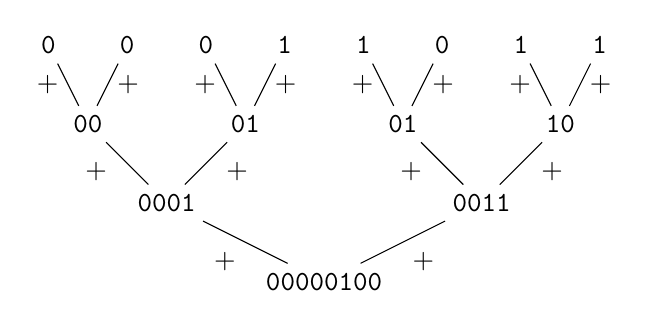
\begin{tikzpicture}[xscale = 0.5, font = \ttfamily]
        \node (n00) at ( 0, 3) {0};
        \node (n01) at ( 2, 3) {0};
        \node (n02) at ( 4, 3) {0};
        \node (n03) at ( 6, 3) {1};
        \node (n04) at ( 8, 3) {1};
        \node (n05) at (10, 3) {0};
        \node (n06) at (12, 3) {1};
        \node (n07) at (14, 3) {1};
        \node (n10) at ( 1, 2) {00};
        \node (n11) at ( 5, 2) {01};
        \node (n12) at ( 9, 2) {01};
        \node (n13) at (13, 2) {10};
        \node (n20) at ( 3, 1) {0001};
        \node (n21) at (11, 1) {0011};
        \node (n30) at ( 7, 0) {00000100};
        \draw (n00) -- node [pos = 0.50, anchor = east] {$+$} (n10);
        \draw (n01) -- node [pos = 0.50, anchor = west] {$+$} (n10);
        \draw (n02) -- node [pos = 0.50, anchor = east] {$+$} (n11);
        \draw (n03) -- node [pos = 0.50, anchor = west] {$+$} (n11);
        \draw (n04) -- node [pos = 0.50, anchor = east] {$+$} (n12);
        \draw (n05) -- node [pos = 0.50, anchor = west] {$+$} (n12);
        \draw (n06) -- node [pos = 0.50, anchor = east] {$+$} (n13);
        \draw (n07) -- node [pos = 0.50, anchor = west] {$+$} (n13);
        \draw (n10) -- node [pos = 0.25, anchor = north east] {$+$} (n20);
        \draw (n11) -- node [pos = 0.25, anchor = north west] {$+$} (n20);
        \draw (n12) -- node [pos = 0.25, anchor = north east] {$+$} (n21);
        \draw (n13) -- node [pos = 0.25, anchor = north west] {$+$} (n21);
        \draw (n20) -- node [pos = 0.50, anchor = north east] {$+$} (n30);
        \draw (n21) -- node [pos = 0.50, anchor = north west] {$+$} (n30);
    \end{tikzpicture}
\end{center}

Listing \ref{lst:arch:popcnt_bin} shows a very efficient implementation.  It
uses a technique known as \textit{SIMD Within A Register} (SWAR), meaning a
single register is treated as several groups of data and each calculation is
done for all of those groups in a single instruction.  This implementation is
very generic and works for types of any width.  Figure \ref{fig:arch:popcnt_bin}
shows the masks and shift operations involved in each step for an 8-bit number.

\begin{figure}[ht]
    \vspace{-\baselineskip}
    \begin{subfigure}[t]{0.7\textwidth}
        \lstinputlisting[
            style=c++,
            firstline=113,
            lastline=133,
            label={lst:arch:popcnt_bin},
            caption={$\log_2$ \texttt{popcnt}},
        ]{arch/bit/popcnt.cpp}
    \end{subfigure}
    \begin{subfigure}[t]{0.275\textwidth}
        \begin{lstlisting}[style=x86]
mov   eax, edi
shr   edi, 1
and   eax, 0x55555555
and   edi, 0x55555555
add   eax, edi
mov   edx, eax
shr   edx, 0x2
and   eax, 0x33333333
and   edx, 0x33333333
add   edx, eax
mov   eax, edx
shr   eax, 0x4
and   edx, 0xf0f0f0f
and   eax, 0xf0f0f0f
add   eax, edx
mov   edx, eax
shr   edx, 0x8
and   eax, 0xff00ff
and   edx, 0xff00ff
add   edx, eax
movzx eax, dx
shr   edx, 0x10
add   eax, edx
ret
        \end{lstlisting}
    \end{subfigure}
    \vspace{-\baselineskip}
\end{figure}

\begin{figure}[p]
    \centering
    \begin{tikzpicture}[>={Stealth[round]}, font = \ttfamily]
    \node (n0) [draw] at (0, 0) {0 0 0 1 1 0 1 1};
    \node (shift0) [right = 1.5 of n0] {0 0 0 0 1 1 0 1};
    \node (and0_0) [draw, circle, below = 0.5 of n0] {\&};
    \node (and0_1) [draw, circle, below = 0.5 of shift0] {\&};
    \node (mask0) [right = 0.45 of and0_0] {0 1 0 1 0 1 0 1};
    \node (n0_0) [below = 0.5 of and0_0] {00 01 00 01};
    \node (n0_1) [below = 0.5 of and0_1] {00 00 01 01};
    \node (p0) [draw, circle, below = 0.5 of n0_0] {$+$};
    \node (n1) [draw, below = 0.5 of p0] {00 01 01 10};
    \node (shift1)
        at ($ (0, 0)!(shift0)!(1, 0) + (0, 0)!(n1)!(0, 1) $)
        {00 00 01 01};
    \node (and1_0) [draw, circle, below = 0.5 of n1] {\&};
    \node (and1_1) [draw, circle, below = 0.5 of shift1] {\&};
    \node (mask1)
        at ($ (0, 0)!(mask0)!(1, 0) + (0, 0)!(and1_0)!(0, 1) $)
        {00 11 00 11};
    \node (n1_0) [below = 0.5 of and1_0] {0001 0010};
    \node (n1_1) [below = 0.5 of and1_1] {0000 0001};
    \node (p1) [draw, circle, below = 0.5 of n1_0] {$+$};
    \node (n2) [draw, below = 0.5 of p1] {0001 0011};
    \node (shift2)
        at ($ (0, 0)!(shift0)!(1, 0) + (0, 0)!(n2)!(0, 1) $)
        {0000 0001};
    \node (and2_0) [draw, circle, below = 0.5 of n2)] {\&};
    \node (and2_1) [draw, circle, below = 0.5 of shift2)] {\&};
    \node (mask2)
        at ($ (0, 0)!(mask0)!(1, 0) + (0, 0)!(and2_0)!(0, 1) $)
        {0000 1111};
    \node (n2_0) [below = 0.5 of and2_0] {00000011};
    \node (n2_1) [below = 0.5 of and2_1] {00000001};
    \node (p2) [draw, circle, below = 0.5 of n2_0] {$+$};
    \node (s) [draw, below = 0.5 of p2] {00000100};
    \draw[->] ($ (n0) + (0, 1) $) -- (n0);
    \draw[->] (n0) -- node [pos = 0.5, anchor = south] {>{}>1} (shift0);
    \draw (n0) -- (and0_0);
    \draw (shift0) -- (and0_1);
    \draw (mask0) -- (and0_0);
    \draw (mask0) -- (and0_1);
    \draw[->] (and0_0) -- (n0_0);
    \draw[->] (and0_1) -- (n0_1);
    \draw (n0_0) -- (p0);
    \draw (n0_1) |- (p0);
    \draw[->] (p0.south) -- +(0, -0.25) -| (n1.north);
    \draw (n1) -- (and1_0);
    \draw (shift1) -- (and1_1);
    \draw (mask1) -- (and1_0);
    \draw (mask1) -- (and1_1);
    \draw[->] (and1_0) -- (n1_0);
    \draw[->] (and1_1) -- (n1_1);
    \draw[->] (n1) -- node [pos = 0.5, anchor = south] {>{}>2} (shift1);
    \draw (n1_0) -- (p1);
    \draw (n1_1) |- (p1);
    \draw[->] (p1.south) -- +(0, -0.25) -| (n2.north);
    \draw[->] (n2) -- node [pos = 0.5, anchor = south] {>{}>4} (shift2);
    \draw (n2) -- (and2_0);
    \draw (shift2) -- (and2_1);
    \draw (mask2) -- (and2_0);
    \draw (mask2) -- (and2_1);
    \draw[->] (and2_0) -- (n2_0);
    \draw[->] (and2_1) -- (n2_1);
    \draw (n2_0) -- (p2);
    \draw (n2_1) |- (p2);
    \draw[->] (p2) -- (s);
\end{tikzpicture}

    \caption{$\log_2$ \texttt{popcnt} for an 8-bit number}
    \label{fig:arch:popcnt_bin}
\end{figure}

\paragraph{CSA}

Performing a population count of several integer values can be a simple matter
of adding the counts of each, but a more efficient method is to use a Carry-Save
Adder (CSA).  This is a circuit used to implement one-digit binary addition
(section \secrefpar{subsubsec:arch:add} shows similar circuits).  It takes three
bits as input (the two values and the previous carry) and has two bits as output
(the sum and the carry) --- it in effect compresses three bits into two.

\begin{wrapfigure}{r}{0.2\textwidth}
    \vspace{-2\baselineskip}
    \begin{lstlisting}[
        label={lst:arch:csa},
        caption={CSA},
    ]
 1111 0000 v0
 1100 1100 v1
+1010 1010 v2
 ---------
 1110 1000 carry
 1001 0110 sum
    \end{lstlisting}
\end{wrapfigure}

This can be used to operate on three values at a time --- one accumulator and
two of the input integers.  The CSA is used to combine bits in the same position
in each of the three inputs.  These circuits can be connected in many ways, and
some result in better performance for certain types of inputs.  Listing
\ref{lst:arch:popcnt_csa} shows a simple implementation.

\begin{figure}[ht]
    \vspace{-\baselineskip}
    \lstinputlisting[
        style=c++,
        firstline=139,
        lastline=157,
        label={lst:arch:popcnt_csa},
        caption={\texttt{popcnt} using a CSA},
    ]{arch/bit/popcnt.cpp}
    \vspace{-\baselineskip}
\end{figure}

\subsection{Binary mask}

One very useful construct when dealing with binary data is the \textit{binary
mask}.  This mask is very similar to a \textit{boolean} value in that it has
only two possible values, but instead of representing the \texttt{true} value as
\texttt{1}, a value where all bits are set to \texttt{1} is used instead.  For
example, for a 4-bit binary number:

\begin{center}
    \begin{tabular}{l|cc}
        & \texttt{bool} & mask \\
        \hline
        \texttt{true}  & \texttt{0001} & \texttt{1111} \\
        \texttt{false} & \texttt{0000} & \texttt{0000} \\
    \end{tabular}
\end{center}

This type of mask is used extensively in programs which do logical and numeric
extensively, since they can be combined with other operations to very
efficiently implement branch-less conditionals, selections, etc.  While boolean
results in languages such as C yield the traditional \texttt{bool} values, whose
stored value is dictated to be either \texttt{0} or \texttt{1}, converting
between these two representations can be done very simply and
efficiently\footnotemark:

\footnotetext{
    \ident{to\_bool} could equally be implemented as \texttt{m \& 1}, which
    would generate an \texttt{and} instruction.  The implementation shown here
    is simpler and generalizes to more than pure binary masks, but both can be
    useful depending on the context.
}

\begin{multicols}{2}
    \begin{lstlisting}[style=c]
bool to_bool(u32 m) {
    return m;
}

u32 to_mask(bool b) {
    return -b;
}
    \end{lstlisting}
    \columnbreak
    \begin{lstlisting}[style=x86]
to_bool:
    test  edi, edi
    setne al
    ret
to_mask:
    movzx eax, dil
    neg   eax
    ret
    \end{lstlisting}
\end{multicols}
\vspace{-\baselineskip}

It should be noted that the generated code shown on the right gives an idea of
how these operations can be translated to machine code, but is very artificial.
Other than the additional requirements of the calling convention, there are a
variety of ways to generate both types of values from ALU operations.  The
actual code generated when these operations are combined with those preceding
and succeeding them will be highly variable, but will invariably be composed of
simple, elemental instructions.  In particular, very rarely will they generate a
combination of a conditional and jump instructions.  Compilers can generally
turn this sort of operations into very efficient code.  For example, if the
input is a regular integer, not a \texttt{bool}:

\begin{multicols}{2}
    \begin{lstlisting}[style=c]
u32 to_mask_u32(u32 x) {
    return to_mask(x);
}
    \end{lstlisting}
    \columnbreak
    \begin{lstlisting}[style=x86]
to_mask_u32:
    neg edi
    sbb eax, eax
    ret
    \end{lstlisting}
\end{multicols}

\subsection{From another bit}

This example (listing \ref{lst:arch:set_bit0}) shows a case where a binary mask
is advantageous.  It sets the value of a given bit in a byte based on the value
of another.  This might be used to change a flag in a bit set based on another.

\begin{figure}[ht]
    \centering
    \vspace{-\baselineskip}
    \begin{subfigure}[t]{0.5\textwidth}
        \lstinputlisting[
            style=c++,
            firstline=19,
            lastline=23,
            label={lst:arch:set_bit0},
            caption={Setting a bit based on another},
        ]{arch/bit/bit.cpp}
    \end{subfigure}
    \hspace{2em}
    \begin{subfigure}[t]{0.2\textwidth}
        \begin{lstlisting}[style=x86]
mov eax, edi
shr al, 4
and eax, 1
neg eax
xor eax, edi
and eax, 4
xor eax, edi
ret
        \end{lstlisting}
    \end{subfigure}
    \vspace{-\baselineskip}
\end{figure}

The binary mask allows the code to operate independently of the position of the
two bits.  In particular, they could be values provided at run time and a
similar sequence of operations could be used (listing \ref{lst:arch:set_bit1}).

\begin{figure}[ht]
    \centering
    \vspace{-\baselineskip}
    \begin{subfigure}[t]{0.5\textwidth}
        \lstinputlisting[
            style=c++,
            firstline=29,
            lastline=32,
            label={lst:arch:set_bit1},
            caption={Setting a bit based on another (param.)},
        ]{arch/bit/bit.cpp}
    \end{subfigure}
    \hspace{2em}
    \begin{subfigure}[t]{0.2\textwidth}
        \begin{lstlisting}[style=x86]
test  sil, dil
setne al
neg   eax
xor   eax, edi
and   eax, edx
xor   eax, edi
ret
        \end{lstlisting}
    \end{subfigure}
    \vspace{-\baselineskip}
\end{figure}

\subsection{Exercises}

\begin{enumerate}[label*=\arabic*.]
    \item
        \label{ex:arch:width_type}
        The return value of the \texttt{popcnt} function in listing
        \ref{lst:arch:blsr} is \texttt{int}.
        \begin{enumerate}[label*=\arabic*.]
            \item
                \label{ex:arch:width_type:range}
                Does that provide an acceptable range of values?  If not, what
                type would be most appropriate for the return value?  Would the
                answer be different if we wanted to optimize for calculation
                speed or data size?  What is the relationship between the type
                of the input and range of possible returned values?
            \item
                \label{ex:arch:width_type:impl}
                Write a type metafunction (v. section \secrefpar{sec:c++:meta})
                that returns the smallest type able to store the number of bits
                in an unsigned integer of a given type.
        \end{enumerate}
    \item
        \label{ex:arch:chess}
        Describe possible forms of storage for the state of the board in a game
        of chess and their advantages.
\end{enumerate}

\section{Floating-point numbers}

% TODO
% https://randomascii.wordpress.com/2012/01/23/stupid-float-tricks-2/
% https://randomascii.wordpress.com/2012/02/11/they-sure-look-equal/
% https://randomascii.wordpress.com/2012/03/08/float-precisionfrom-zero-to-100-digits-2/
% https://randomascii.wordpress.com/2012/03/11/c-11-stdasync-for-fast-float-format-finding/
% https://randomascii.wordpress.com/2012/02/25/comparing-floating-point-numbers-2012-edition/

The representation of binary floating-point numbers as defined by the IEEE-754
standard is composed of three elements: \begin{enumerate*}[1)] \item sign bit,
\item exponent, and \item mantissa \end{enumerate*}.  The sizes and ranges for
the second and third values depend on the overall storage size reserved for the
number; common sizes are shown in table \ref{tbl:arch:float}.

\begin{table}[ht]
    \centering
    \begin{tabular}{cccccc}
        & Common name & C type & Total bits & Exponent & Mantissa \\
        \hline
        \texttt{f16} & half precision & --- & 16 & 5 & 10 \\
        \texttt{f32} & single precision & \texttt{float} & 32 & 8 & 23 \\
        \texttt{f64} & double precision & \texttt{double} & 64 & 11 & 52 \\
        \texttt{f128} & quadruple precision & \texttt{long double} & 128 & 15
            & 112 \\
    \end{tabular}
    \caption{Common floating-point sizes}
    \label{tbl:arch:float}
\end{table}

Note that the C standard does not require any of the three types in the table,
nor that they be implemented using IEEE-754 (but if they are, those must be the
corresponding types).  Additionally, if 128-bit numbers are not supported,
\texttt{long double} may be implemented as an unspecified ``extended'' format
whose only requirement is greater precision than a \texttt{double} (e.g. the x87
80-bit extended precision format).  Regardless of the size, the value of a
binary floating-point number is always calculated in the same manner:

\begin{align*}
f = s \; b^e m \\
\end{align*}

In reality, these components are not stored in their original form.  The most
significant bit records the sign $s$, just as in one and two's complement
representations (v. section \secrefpar{subsec:arch:ones_twos_comp}).  The base
$b$ is always implicitly 2, and the exponent $e$ is stored with a \textit{bias}
(v. section \secrefpar{subsec:arch:float_exp}).  Only the fractional bits of the
mantissa $m$ are stored, an implicit leading digit of 1 is always added.  Thus,
for a single-precision number (\texttt{f32}), the value based on the stored
components is:

\begin{align*}
    (-1)^s \; 2^{e - 127} \left(1 + m \; 2^{-23}\right) \\
\end{align*}

Where $m$ is the stored bits of the mantissa interpreted as an unsigned integer.
An alternate formulation, where $m_i$ means ``the $i$th bit of the stored
mantissa'', is:

\begin{align*}
    (-1)^s \; 2^{e - 127} \left(1 + \sum_{i=1}^{23} m_{23-i} 2^{-i}\right) \\
\end{align*}

From these equations, the minimum and maximum (absolute) representable values
can be derived.  The minimum value has an exponent of $-126$ and a significand
of $1$ (i.e. the stored mantissa is zero), while the maximum value has an
exponent of $127$ and a mantissa whose bits are all ones:

\begin{align*}
    \texttt{FLT\_MIN} &= \texttt{0 00000001 00000000000000000000000}_2 \\
                      &= \texttt{0080 0000}_{16} \\
                      &= 2^{-126} \\
                      &\approx 1.1754943508223 \times 10^{-38} \\
    \texttt{FLT\_MAX} &= \texttt{0 11111110 11111111111111111111111}_2 \\
                      &= \texttt{7f7f ffff}_{16} \\
                      &= 2^{128} - 2^{128 - 24} \\
                      &\approx 3.4028234663853 \times 10^{38} \\
\end{align*}

The following C code can be used to extract each of the components above from a
single-precision value and reassemble them into the original number.  In the
second part, size limits are disregarded in the calculation of the exponent and
significand for simplicity of demonstration.  The standard library provides
several functions in \texttt{<math.h>} which perform this type of operations;
they are shown in comments next to their equivalent.

\begin{lstlisting}[style=c]
// input
extern float f;
// binary representation
u32 uf;
static_assert(sizeof(uf) == sizeof(f));
memcpy(&uf, &f, sizeof(uf));
// disassemble
const i32 s = uf >> 31; // (bool)signbit(f)
const i32 e = ((uf >> 23) & 0xff) - 127; // ilogbf(f)
const i32 m = uf & 0x7fffff;
// reassemble
const float fs = 1 - (s << 1); // copysignf(1, f)
const float fe = 1 << e; // scalbnf(1, e)
const float fm = 1 + m / 0x1p23f; // 1 + scalbnf(m, -23)
f = fs * fe * fm;
\end{lstlisting}

\subsection{Exponent}

\label{subsec:arch:float_exp}

The representation of the exponent, which can be a negative number, is different
from the ones shown in section \secref{subsec:arch:ones_twos_comp}: the stored
value is instead \textit{biased}.  For single-precision numbers, with 8-bit
exponents, the actual stored value is the exponent plus 127.  Special treatment
is given to numbers with an encoded exponent value of zero (v. section
\secrefpar{subsec:arch:subnormal}) and 255 (the maximum value, used for infinity
and \texttt{NaN} values), so the effective exponent range is $[1, 254] - 127 =
[-126,127]$.  This range has one more value in the non-negative range than the
negative range, also unlike two's complement.

The main advantage of this storage format is that numbers in the normal range
(i.e. excluding \texttt{NaN}s and infinities) can be compared lexicographically
directly in their encoded format as if they were regular signed integers.  This
would not be possible in a complement representation since the (exponent's) sign
bit would place negative numbers after non-negative numbers.

\subsection{Precision}

As any numerical representation in computers, floating-point numbers can
represent only a finite set of values.  However, because of the exponent
multiplication and the fixed number of bits in the mantissa, the range of this
precision is variable.  This is manifested in two ways.  First, if a large
portion of the bits of the mantissa are required to represent the integral part,
few bits will be available for the fractional part, resulting in less precision
for fractional digits.  The absolute precision range also depends on the
magnitude of the number, since the number of bits in the mantissa is constant:
the larger the number, the larger the exponentiated multiplier, and the larger
the gap between each value representable by the mantissa.

A visual conceptualization of the IEEE-754 storage format can be helpful in
understanding these precision limitations.  The significand has an implicit
digit of one, while the mantissa represents fractional digits, meaning the
effective range of the significand is [1, 2).  A crucial observation is that,
for any number whose exponent is $e$ and whose mantissa is all ones, the next
representable value has exponent $e + 1$ and a mantissa of zero\footnotemark.
This means every value which is representable also has a \emph{unique}
representation.

\footnotetext{
    In fact, the bit representation of the number can simply be treated as an
    unsigned integer in this operation, which is equivalent to the standard
    function \texttt{nextafter}, for all values in the range
    $[\texttt{0},\texttt{FLT\_MAX}]$.  Similarly, the same is true in the other
    direction for negative numbers in the range
    $[\texttt{-FLT\_MAX},\texttt{-0}]$, although note that there is no such
    relation in the transition between negative and positive values in either
    direction.  See figure \secref{fig:arch:float_ranges}.}

In this perspective, each exponent value can be seen as a sub-range of the
entire range of representable values (i.e. [\ident{FLT_MIN},\ident{FLT_MAX}]).
Each covers the range $[2^e,2^{e+1})$, where $e$ is the value of the exponent,
and is in turn divided equally into $2^n$ sub-ranges, where $n$ is the number of
bits in the mantissa\footnotemark.  It is thus obvious (hopefully) why the
precision is variable according to the magnitude of the number: each sub-range
has the same number of divisions, so larger sub-ranges will have larger
intervals between each division.

\footnotetext{
    The value of the mantissa can also be considered an \emph{offset} into the
    range denoted by the exponent, or conversely, the exponent can also be seen
    as \emph{shifting} the significant digits of the mantissa.}

As an extreme example, numbers close to \ident{FLT_MAX} have, as shown above, an
exponent of 127.  The smallest number with that exponent is $2^{127}$, which in
unsigned integer notation is \texttt{0x80000000000000000000000000000000}, i.e.
a one followed by 127 zeroes.  In other words, the leading one bit implicit in
the significand is shifted left 127 positions.  The next representable number is
the one where the mantissa has its least significant bit set, i.e. $2^{127} \;
(1 + 2^{-23})$.  The interval between those numbers is $2^{127} \; 2^{-23} =
2^{127-23} = 2^{104}$.  If these numbers are involved in additions/subtractions
with others which contain any extra digits inside this enormous interval, those
digits will be discarded since there is not enough precision in the mantissa to
represent them.  In general, operations between numbers of similar magnitude
have the most precision.

\subsection{Subnormal numbers}

\label{subsec:arch:subnormal}

In order to cover the range $(-\texttt{FLT\_MIN},\texttt{FLT\_MIN})$, IEEE-754
includes as an extension a category of numbers called \textit{subnormal}.  These
numbers have a biased exponent of zero, but their effective exponent is
considered to be one and the implicit leading bit in the significand is not
added.  We can now depict the full range of values representable by
single-precision IEE-754 numbers (figure \ref{fig:arch:float_ranges}).

\subsection{Machine epsilon}

\begin{figure}[p]
    \begin{align*}
        1 \; 11111111 \; 00000000000000000000000_2 &= -\texttt{INFINITY} \\
        1 \; 11111110 \; 11111111111111111111111_2 &= -\texttt{FLT\_MAX}
            = -2^{128} + 2^{128-24} \\
        \vdots \\
        1 \; 01111111 \; 00000000000000000000001_2 &= -1 - 2^{-23} \\
        1 \; 01111111 \; 00000000000000000000000_2 &= -1 \\
        1 \; 01111110 \; 11111111111111111111111_2 &= -1 + 2^{-24} \\
        \vdots \\
        1 \; 00000001 \; 00000000000000000000000_2 &= -\texttt{FLT\_MIN}
            = -2^{-126} \\
        1 \; 00000000 \; 11111111111111111111111_2 &= \text{min. subnormal}
            = -2^{-126} \; (1 + 2^{-23}) \\
        \vdots \\
        1 \; 00000000 \; 00000000000000000000001_2 &= -\texttt{FLT\_TRUE\_MIN}
            = -2^{-127} \; 2^{-23} = -2^{-140} \\
        1 \; 00000000 \; 00000000000000000000000_2 &= -0 \\
        0 \; 00000000 \; 00000000000000000000000_2 &= 0 \\
        0 \; 00000000 \; 00000000000000000000001_2 &= \texttt{FLT\_TRUE\_MIN}
            = 2^{-127} \; 2^{-23} = 2^{-140} \\
        \vdots \\
        0 \; 00000000 \; 11111111111111111111111_2 &= \text{max. subnormal}
            = 2^{-126} \; (1 - 2^{-23}) \\
        0 \; 00000001 \; 00000000000000000000000_2 &= \texttt{FLT\_MIN}
            = 2^{-126} \\
        \vdots \\
        0 \; 01111110 \; 11111111111111111111111_2 &= 1 - 2^{-24} \\
        0 \; 01111111 \; 00000000000000000000000_2 &= 1 \\
        0 \; 01111111 \; 00000000000000000000001_2 &= 1 + 2^{-23} \\
        \vdots \\
        0 \; 11111110 \; 11111111111111111111111_2 &= \texttt{FLT\_MAX}
            = 2^{128} - 2^{128-24} \\
        0 \; 11111111 \; 00000000000000000000000_2 &= \texttt{INFINITY} \\
    \end{align*}
    \caption{Adjacent floating-point ranges}
    \label{fig:arch:float_ranges}
\end{figure}

A standard measurement of the precision of floating-point representations is the
\textit{machine epsilon}: the distance between the value 1 and the next smallest
value that is greater than it, i.e. the smallest value $\epsilon$ which
satisfies $1 + \epsilon \neq 1$.  For an IEEE-754 single-precision number, the
previous section has shown that $\epsilon = 2^{-23}$.

Because the precision of a floating-point number varies according to its
magnitude, this distance increases as a function of the exponent.  In general,
the absolute distance between a floating-point number with exponent $e$ and the
next representable value is $2^e \epsilon$.  This value can be used to calculate
relative error, turn greater-than-or-equal comparisons into greater-than, etc.

\section{Latches}

All logic circuits discussed so far have been directed acyclic graphs: data flow
in a single direction for each connection and any individual signal starts at
one of the inputs and travels through the graph to one of the outputs, never
passing through the same gate more than once.  This is enough to implement
transient computation, such as additions and bitwise operations, as we have
seen, but computers also need to \emph{retain} information for a period of time.
Building components which can do that requires some form of loop where the
current state is used in the computation of the next.

A very simple circuit with that property is an \textit{or} gate whose output is
connected to one of its inputs (figure \ref{fig:arch:or_loop}).  The output of
this circuit will be zero until the input is set.  From that point on, as long
as the circuit is powered, its output will always be on, since the signal that
loops back to the \textit{or} gate is on and that is enough to turn the gate on.

\begin{figure}[p]
    \centering
    \begin{subfigure}{0.24\textwidth}
        \begin{tikzpicture}[{circuit_diagram}]
    \node (or) [or gate] {};
    \node (in) [left = of or.input 1, xshift = 1em] {I};
    \node (or0) [point, right = of or, xshift = -2em] {};
    \node (out) [right = of or0, xshift = -2em] {O};
    \draw (in) -- (or.input 1);
    \draw (or.output) -- (or0);
    \draw (or0) -- (out);
    \draw (or0)
        -- ($
            (0, -0.6)
            + (0, 0)!(or0)!(1, 0)
            + (0, 0)!(or.input 2)!(0, 1)
        $)
        -- ($ (or.input 2) - (0.4, 0.6) $)
        -- ($ (or.input 2) - (0.4, 0) $)
        -- (or.input 2);
\end{tikzpicture}

        \caption{initial state}
    \end{subfigure}
    \begin{subfigure}{0.24\textwidth}
        \begin{tikzpicture}[{circuit_diagram}]
    \node (or) [or gate] {};
    \node (in) [left = of or.input 1, xshift = 1em] {I};
    \node (or0) [point, right = of or, xshift = -2em] {};
    \node (out) [right = of or0, xshift = -2em] {O};
    \draw [red, thick] (in) -- (or.input 1);
    \draw (or.output) -- (or0);
    \draw (or0) -- (out);
    \draw (or0)
        -- ($
            (0, -0.6)
            + (0, 0)!(or0)!(1, 0)
            + (0, 0)!(or.input 2)!(0, 1)
        $)
        -- ($ (or.input 2) - (0.4, 0.6) $)
        -- ($ (or.input 2) - (0.4, 0) $)
        -- (or.input 2);
\end{tikzpicture}

        \caption{input is set}
    \end{subfigure}
    \begin{subfigure}{0.24\textwidth}
        \begin{tikzpicture}[{circuit_diagram}]
    \node (or) [or gate] {};
    \node (in) [left = of or.input 1, xshift = 1em] {I};
    \node (or0) [point, right = of or, xshift = -2em] {};
    \node (out) [right = of or0, xshift = -2em] {O};
    \draw [red, thick] (in) -- (or.input 1);
    \draw [red, thick] (or.output) -- (or0);
    \draw [red, thick] (or0) -- (out);
    \draw [red, thick] (or0)
        -- ($
            (0, -0.6)
            + (0, 0)!(or0)!(1, 0)
            + (0, 0)!(or.input 2)!(0, 1)
        $)
        -- ($ (or.input 2) - (0.4, 0.6) $)
        -- ($ (or.input 2) - (0.4, 0) $)
        -- (or.input 2);
\end{tikzpicture}

        \caption{\textit{or} propagates}
    \end{subfigure}
    \begin{subfigure}{0.24\textwidth}
        \begin{tikzpicture}[{circuit_diagram}]
    \node (or) [or gate] {};
    \node (in) [left = of or.input 1, xshift = 1em] {I};
    \node (or0) [point, right = of or, xshift = -2em] {};
    \node (out) [right = of or0, xshift = -2em] {O};
    \draw (in) -- (or.input 1);
    \draw [red, thick] (or.output) -- (or0);
    \draw [red, thick] (or0) -- (out);
    \draw [red, thick] (or0)
        -- ($
            (0, -0.6)
            + (0, 0)!(or0)!(1, 0)
            + (0, 0)!(or.input 2)!(0, 1)
        $)
        -- ($ (or.input 2) - (0.4, 0.6) $)
        -- ($ (or.input 2) - (0.4, 0) $)
        -- (or.input 2);
\end{tikzpicture}

        \caption{input is cleared}
    \end{subfigure}
    \caption{\textit{or} gate with a loop}
    \label{fig:arch:or_loop}
\end{figure}

Figure \ref{fig:arch:sr_latch} shows an improved version of this concept where
two \textit{nor} gates are interconnected.  Initially, one of the two outputs,
which are complements, is set (which one depends on propagation delays, this is
a hardware race condition).

\begin{figure}[p]
    \centering
    \begin{subfigure}{0.25\textwidth}
        \begin{tikzpicture}[scale = 0.75, circuit logic CDH, huge circuit symbols]
    \node (q)  at (0, 2) {Q};
    \node (nq) at (0, 0) {$\bar{\text{Q}}$};
    \node (nor0) [nor gate, left = of q] {};
    \node (nor1) [nor gate, left = of nq] {};
    \node (p0) [point, right = of nor0.output, xshift = -1.75em] {};
    \node (p1) [point, right = of nor1.output, xshift = -1.75em] {};
    \node (r) [left = of nor0.input 1, xshift = 1em] {R};
    \node (s) [left = of nor1.input 2, xshift = 1em] {S};
    \draw (r) -- (nor0.input 1);
    \draw (s) -- (nor1.input 2);
    \draw [red, thick] (p0)
        -- ($ (nor1.input 1) + (-1em, 1em) $)
        -- ($ (nor1.input 1) - (1em, 0) $)
        -- (nor1.input 1);
    \draw (p1)
        -- ($ (nor0.input 2) - (1em, 1em) $)
        -- ($ (nor0.input 2) - (1em, 0) $)
        -- (nor0.input 2);
    \draw [red, thick] (nor0.output) -- (q);
    \draw (nor1.output) -- (nq);
\end{tikzpicture}

        \caption{initial state}
    \end{subfigure}
    \begin{subfigure}{0.25\textwidth}
        \begin{tikzpicture}[scale = 0.75, circuit logic CDH, huge circuit symbols]
    \node (q)  at (0, 2) {Q};
    \node (nq) at (0, 0) {$\bar{\text{Q}}$};
    \node (nor0) [nor gate, left = of q] {};
    \node (nor1) [nor gate, left = of nq] {};
    \node (p0) [point, right = of nor0.output, xshift = -1.75em] {};
    \node (p1) [point, right = of nor1.output, xshift = -1.75em] {};
    \node (r) [left = of nor0.input 1, xshift = 1em] {R};
    \node (s) [left = of nor1.input 2, xshift = 1em] {S};
    \draw [red, thick] (r) -- (nor0.input 1);
    \draw (s) -- (nor1.input 2);
    \draw [red, thick] (p0)
        -- ($ (nor1.input 1) + (-1em, 1em) $)
        -- ($ (nor1.input 1) - (1em, 0) $)
        -- (nor1.input 1);
    \draw (p1)
        -- ($ (nor0.input 2) - (1em, 1em) $)
        -- ($ (nor0.input 2) - (1em, 0) $)
        -- (nor0.input 2);
    \draw [red, thick] (nor0.output) -- (q);
    \draw (nor1.output) -- (nq);
\end{tikzpicture}

        \caption{reset is raised}
    \end{subfigure}
    \begin{subfigure}{0.25\textwidth}
        \begin{tikzpicture}[scale = 0.75, circuit logic CDH, huge circuit symbols]
    \node (q)  at (0, 2) {Q};
    \node (nq) at (0, 0) {$\bar{\text{Q}}$};
    \node (nor0) [nor gate, left = of q] {};
    \node (nor1) [nor gate, left = of nq] {};
    \node (p0) [point, right = of nor0.output, xshift = -1.75em] {};
    \node (p1) [point, right = of nor1.output, xshift = -1.75em] {};
    \node (r) [left = of nor0.input 1, xshift = 1em] {R};
    \node (s) [left = of nor1.input 2, xshift = 1em] {S};
    \draw [red, thick] (r) -- (nor0.input 1);
    \draw (s) -- (nor1.input 2);
    \draw (p0)
        -- ($ (nor1.input 1) + (-1em, 1em) $)
        -- ($ (nor1.input 1) - (1em, 0) $)
        -- (nor1.input 1);
    \draw (p1)
        -- ($ (nor0.input 2) - (1em, 1em) $)
        -- ($ (nor0.input 2) - (1em, 0) $)
        -- (nor0.input 2);
    \draw (nor0.output) -- (q);
    \draw (nor1.output) -- (nq);
\end{tikzpicture}

        \caption{Q is cleared}
    \end{subfigure}
    \\~\\~\\
    \begin{subfigure}{0.25\textwidth}
        \begin{tikzpicture}[scale = 0.75, circuit logic CDH, huge circuit symbols]
    \node (q)  at (0, 2) {Q};
    \node (nq) at (0, 0) {$\bar{\text{Q}}$};
    \node (nor0) [nor gate, left = of q] {};
    \node (nor1) [nor gate, left = of nq] {};
    \node (p0) [point, right = of nor0.output, xshift = -1.75em] {};
    \node (p1) [point, right = of nor1.output, xshift = -1.75em] {};
    \node (r) [left = of nor0.input 1, xshift = 1em] {R};
    \node (s) [left = of nor1.input 2, xshift = 1em] {S};
    \draw [red, thick] (r) -- (nor0.input 1);
    \draw (s) -- (nor1.input 2);
    \draw (p0)
        -- ($ (nor1.input 1) + (-1em, 1em) $)
        -- ($ (nor1.input 1) - (1em, 0) $)
        -- (nor1.input 1);
    \draw [red, thick] (p1)
        -- ($ (nor0.input 2) - (1em, 1em) $)
        -- ($ (nor0.input 2) - (1em, 0) $)
        -- (nor0.input 2);
    \draw (nor0.output) -- (q);
    \draw [red, thick] (nor1.output) -- (nq);
\end{tikzpicture}

        \caption{$\bar{\text{Q}}$ is set}
    \end{subfigure}
    \begin{subfigure}{0.25\textwidth}
        \begin{tikzpicture}[scale = 0.75, circuit logic CDH, huge circuit symbols]
    \node (q)  at (0, 2) {Q};
    \node (nq) at (0, 0) {$\bar{\text{Q}}$};
    \node (nor0) [nor gate, left = of q] {};
    \node (nor1) [nor gate, left = of nq] {};
    \node (p0) [point, right = of nor0.output, xshift = -1.75em] {};
    \node (p1) [point, right = of nor1.output, xshift = -1.75em] {};
    \node (r) [left = of nor0.input 1, xshift = 1em] {R};
    \node (s) [left = of nor1.input 2, xshift = 1em] {S};
    \draw (r) -- (nor0.input 1);
    \draw (s) -- (nor1.input 2);
    \draw (p0)
        -- ($ (nor1.input 1) + (-1em, 1em) $)
        -- ($ (nor1.input 1) - (1em, 0) $)
        -- (nor1.input 1);
    \draw [red, thick] (p1)
        -- ($ (nor0.input 2) - (1em, 1em) $)
        -- ($ (nor0.input 2) - (1em, 0) $)
        -- (nor0.input 2);
    \draw (nor0.output) -- (q);
    \draw [red, thick] (nor1.output) -- (nq);
\end{tikzpicture}

        \caption{reset is lowered}
    \end{subfigure}
    \begin{subfigure}{0.25\textwidth}
        \begin{tikzpicture}[scale = 0.75, circuit logic CDH, huge circuit symbols]
    \node (q)  at (0, 2) {Q};
    \node (nq) at (0, 0) {$\bar{\text{Q}}$};
    \node (nor0) [nor gate, left = of q] {};
    \node (nor1) [nor gate, left = of nq] {};
    \node (p0) [point, right = of nor0.output, xshift = -1.75em] {};
    \node (p1) [point, right = of nor1.output, xshift = -1.75em] {};
    \node (r) [left = of nor0.input 1, xshift = 1em] {R};
    \node (s) [left = of nor1.input 2, xshift = 1em] {S};
    \draw (r) -- (nor0.input 1);
    \draw [red, thick] (s) -- (nor1.input 2);
    \draw (p0)
        -- ($ (nor1.input 1) + (-1em, 1em) $)
        -- ($ (nor1.input 1) - (1em, 0) $)
        -- (nor1.input 1);
    \draw [red, thick] (p1)
        -- ($ (nor0.input 2) - (1em, 1em) $)
        -- ($ (nor0.input 2) - (1em, 0) $)
        -- (nor0.input 2);
    \draw (nor0.output) -- (q);
    \draw [red, thick] (nor1.output) -- (nq);
\end{tikzpicture}

        \caption{set is raised}
    \end{subfigure}
    \\~\\~\\
    \begin{subfigure}{0.25\textwidth}
        \begin{tikzpicture}[scale = 0.75, circuit logic CDH, huge circuit symbols]
    \node (q)  at (0, 2) {Q};
    \node (nq) at (0, 0) {$\bar{\text{Q}}$};
    \node (nor0) [nor gate, left = of q] {};
    \node (nor1) [nor gate, left = of nq] {};
    \node (p0) [point, right = of nor0.output, xshift = -1.75em] {};
    \node (p1) [point, right = of nor1.output, xshift = -1.75em] {};
    \node (r) [left = of nor0.input 1, xshift = 1em] {R};
    \node (s) [left = of nor1.input 2, xshift = 1em] {S};
    \draw (r) -- (nor0.input 1);
    \draw [red, thick] (s) -- (nor1.input 2);
    \draw (p0)
        -- ($ (nor1.input 1) + (-1em, 1em) $)
        -- ($ (nor1.input 1) - (1em, 0) $)
        -- (nor1.input 1);
    \draw (p1)
        -- ($ (nor0.input 2) - (1em, 1em) $)
        -- ($ (nor0.input 2) - (1em, 0) $)
        -- (nor0.input 2);
    \draw (nor0.output) -- (q);
    \draw (nor1.output) -- (nq);
\end{tikzpicture}

        \caption{$\bar{\text{Q}}$ is cleared}
    \end{subfigure}
    \begin{subfigure}{0.25\textwidth}
        \begin{tikzpicture}[scale = 0.75, circuit logic CDH, huge circuit symbols]
    \node (q)  at (0, 2) {Q};
    \node (nq) at (0, 0) {$\bar{\text{Q}}$};
    \node (nor0) [nor gate, left = of q] {};
    \node (nor1) [nor gate, left = of nq] {};
    \node (p0) [point, right = of nor0.output, xshift = -1.75em] {};
    \node (p1) [point, right = of nor1.output, xshift = -1.75em] {};
    \node (r) [left = of nor0.input 1, xshift = 1em] {R};
    \node (s) [left = of nor1.input 2, xshift = 1em] {S};
    \draw (r) -- (nor0.input 1);
    \draw [red, thick] (s) -- (nor1.input 2);
    \draw [red, thick] (p0)
        -- ($ (nor1.input 1) + (-1em, 1em) $)
        -- ($ (nor1.input 1) - (1em, 0) $)
        -- (nor1.input 1);
    \draw (p1)
        -- ($ (nor0.input 2) - (1em, 1em) $)
        -- ($ (nor0.input 2) - (1em, 0) $)
        -- (nor0.input 2);
    \draw [red, thick] (nor0.output) -- (q);
    \draw (nor1.output) -- (nq);
\end{tikzpicture}

        \caption{Q is set}
    \end{subfigure}
    \begin{subfigure}{0.25\textwidth}
        \begin{tikzpicture}[scale = 0.75, circuit logic CDH, huge circuit symbols]
    \node (q)  at (0, 2) {Q};
    \node (nq) at (0, 0) {$\bar{\text{Q}}$};
    \node (nor0) [nor gate, left = of q] {};
    \node (nor1) [nor gate, left = of nq] {};
    \node (p0) [point, right = of nor0.output, xshift = -1.75em] {};
    \node (p1) [point, right = of nor1.output, xshift = -1.75em] {};
    \node (r) [left = of nor0.input 1, xshift = 1em] {R};
    \node (s) [left = of nor1.input 2, xshift = 1em] {S};
    \draw (r) -- (nor0.input 1);
    \draw (s) -- (nor1.input 2);
    \draw [red, thick] (p0)
        -- ($ (nor1.input 1) + (-1em, 1em) $)
        -- ($ (nor1.input 1) - (1em, 0) $)
        -- (nor1.input 1);
    \draw (p1)
        -- ($ (nor0.input 2) - (1em, 1em) $)
        -- ($ (nor0.input 2) - (1em, 0) $)
        -- (nor0.input 2);
    \draw [red, thick] (nor0.output) -- (q);
    \draw (nor1.output) -- (nq);
\end{tikzpicture}

        \caption{set is lowered}
    \end{subfigure}
    \caption{SR latch}
    \label{fig:arch:sr_latch}
\end{figure}

Assuming that is the gate associated with R, the circuit will reach a stable
state where Q is set.  Raising and lowering S at this point has no effect, as
the \textit{nor} gate will not propagate the signal as long as the crossed
connection is on.  Raising R (short for \textit{reset}) will clear Q, but also
clear the input to the other \textit{nor} gate.  This will cause both
$\bar{\text{Q}}$ and one of the inputs to the first \textit{nor} gate to be set.
R can be lowered and raising and lowering it again at this point has no effect.
Raising S (short for \textit{set}) has the opposite effect: $\bar{\text{Q}}$ and
the first gate are cleared, Q is set, and we are back at the initial state.

From this we can observe that the circuit has two stable states: Q set and
$\bar{\text{Q}}$ cleared, or vice versa.  Raising R or S transitions the circuit
from one state to the other, which will be maintained until the next transition.
Components that exhibit this type of behavior are called \textit{latches}, as
the output is locked when an operation is performed and state is preserved.
This particular circuit is called an \textit{SR latch}, due to its two inputs.

The \textit{D latch} (figure \ref{fig:arch:d_latch}) is a similar circuit which
uses a single input instead of a reset/set pair.  Two additions to the SR latch
accomplish this.  First, a single input D (short for \textit{data}) is connected
to R and S, with R going through a \textit{not} gate.  State is now no longer
retained since toggling D immediately raises one of R or S.  An input EN (short
for \textit{enable}) is added so that transitions occur only when it is on.
This is done by placing two \textit{and} gates between R/S and the latch, which
are also connected to EN.

\begin{figure}[p]
    \centering
    \begin{tikzpicture}[circuit logic CDH, huge circuit symbols]
    \node (q)  at (6, 2) {Q};\node (nq) at (6, 0) {$\bar{\text{Q}}$};
    \node (nor0) [nor gate, left = of q] {};
    \node (nor1) [nor gate, left = of nq] {};
    \node (and0) [and gate, left = of nor0.input 1, xshift = 1em] {R};
    \node (and1) [and gate, left = of nor1.input 2, xshift = 1em] {S};
    \node (p0) [point, right = of nor0.output, xshift = -1.75em] {};
    \node (p1) [point, right = of nor1.output, xshift = -1.75em] {};
    \node (not) [
        not gate, circuit symbol unit = 0.4em,
        left = of and0.input 1, xshift = 1em,
    ] {};
    \node (d0) [point] at (0, 1) {};
    \node (d) [left = of d0, xshift = 2em] {D};
    \node (en0) [point] at (1.25, 1) {};
    \node (en) [left = of en0, xshift = 2em] {EN};
    \draw (d) -- (d0);
    \draw (d0) |- (not) -- (and0.input 1);
    \draw (d0) |- (and1.input 2);
    \draw (en) -- (en0);
    \draw (en0) |- (and0.input 2);
    \draw (en0) |- (and1.input 1);
    \draw (and0) -- (nor0.input 1);
    \draw (and1) -- (nor1.input 2);
    \draw (p0)
        -- ($ (nor1.input 1) + (-1em, 1em) $)
        -- ($ (nor1.input 1) - (1em, 0) $)
        -- (nor1.input 1);
    \draw (p1)
        -- ($ (nor0.input 2) - (1em, 1em) $)
        -- ($ (nor0.input 2) - (1em, 0) $)
        -- (nor0.input 2);
    \draw (nor0.output) -- (q);
    \draw (nor1.output) -- (nq);
    \draw[-, dotted]
        ($ (and1)    + (-0.75em, -1.50em) $)
        -- node[below] {latch} +(12.25em, 0)
        -- ($ (and0) + (11.50em,  1.50em) $)
        -- ($ (and0) + (-0.75em,  1.50em) $)
        -- ($ (and1) + (-0.75em, -1.50em) $);
\end{tikzpicture}

    \caption{D latch}
    \label{fig:arch:d_latch}
\end{figure}

These additions create a circuit that will change its state based on the
combination of both its inputs.  Figure \ref{fig:arch:d_latch_clock} shows the
relationship between changes to D/EN and the output of a D latch over time.
Whenever EN is on, Q follows the value of D (green lines).  Conversely, changing
D while EN is off has no effect on the value of Q (red lines).  This type of
latch is called a \textit{transparent latch}, as the value of the input is
constantly forwarded to the output as long as the enable signal is on.

\begin{figure}[ht]
    \centering
    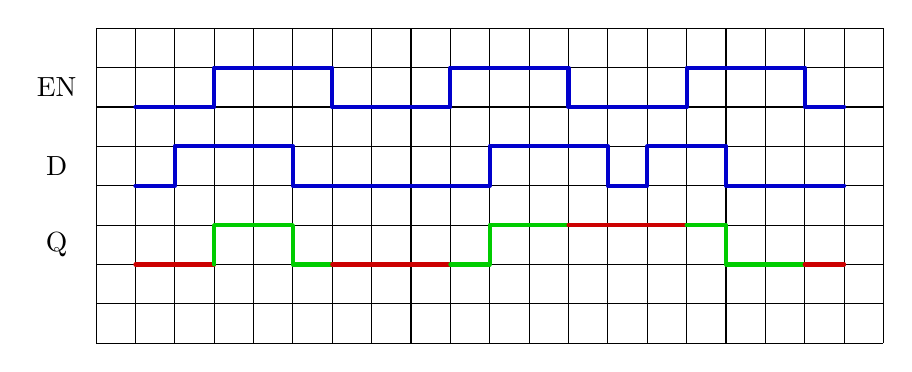
\begin{tikzpicture}[
        scale = 0.5,
        line/.style={line width = 0.15em, line join = round, line cap = round},
        input/.style={line, blue!80!black},
        on/.style={line, green!80!black},
        off/.style={line, red!80!black},
    ]
        \draw[step = 1] (0, 0) grid (20, 8);
        \node at (-1, 6.5) {EN};
        \node at (-1, 4.5) {D};
        \node at (-1, 2.5) {Q};
        \draw[input]
            (1, 6) -- (3, 6) -- (3, 7) -- (6, 7) -- (6, 6) -- (9, 6) -- (9, 6)
            -- (9, 7) -- (12, 7) -- (12, 6) -- (15, 6) -- (15, 7) -- (18, 7)
            -- (18, 6) -- (19, 6);
        \draw[input]
            (1, 4) -- (2, 4) -- (2, 5) -- (5, 5) -- (5, 4) -- (10, 4) -- (10, 5)
            -- (13, 5) -- (13, 4) -- (14, 4) -- (14, 5) -- (16, 5) -- (16, 4)
            -- (19, 4);
        \draw[off] ( 1, 2) -- ( 3, 2);
        \draw[on]  ( 3, 2) -- ( 3, 3) -- ( 5, 3) -- ( 5, 2) -- (6, 2);
        \draw[off] ( 6, 2) -- ( 9, 2);
        \draw[on]  ( 9, 2) -- (10, 2) -- (10, 3) -- (12, 3);
        \draw[off] (12, 3) -- (15, 3);
        \draw[on]  (15, 3) -- (16, 3) -- (16, 2) -- (18, 2);
        \draw[off] (18, 2) -- (19, 2);
    \end{tikzpicture}
    \caption{D latch timing diagram}
    \label{fig:arch:d_latch_clock}
\end{figure}

\begin{figure}[ht]
    \centering
    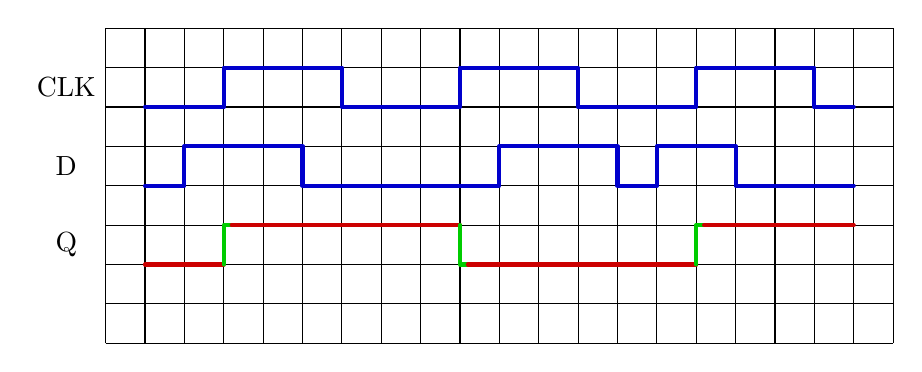
\begin{tikzpicture}[
        scale = 0.5,
        line/.style={line width = 0.15em, line join = round, line cap = round},
        input/.style={line, blue!80!black},
        on/.style={line, green!80!black},
        off/.style={line, red!80!black},
    ]
        \draw[step = 1] (0, 0) grid (20, 8);
        \node at (-1, 6.5) {CLK};
        \node at (-1, 4.5) {D};
        \node at (-1, 2.5) {Q};
        \draw[input]
            (1, 6) -- (3, 6) -- (3, 7) -- (6, 7) -- (6, 6) -- (9, 6) -- (9, 6)
            -- (9, 7) -- (12, 7) -- (12, 6) -- (15, 6) -- (15, 7) -- (18, 7)
            -- (18, 6) -- (19, 6);
        \draw[input]
            (1, 4) -- (2, 4) -- (2, 5) -- (5, 5) -- (5, 4) -- (10, 4) -- (10, 5)
            -- (13, 5) -- (13, 4) -- (14, 4) -- (14, 5) -- (16, 5) -- (16, 4)
            -- (19, 4);
        \draw[off] ( 1.0, 2) -- ( 3, 2);
        \draw[on]  ( 3.0, 2) -- ( 3, 3) -- (3.2, 3);
        \draw[off] ( 3.2, 3) -- ( 9, 3);
        \draw[on]  ( 9.0, 3) -- ( 9, 2) -- (9.2, 2);
        \draw[off] ( 9.2, 2) -- (15, 2);
        \draw[on]  (15,   2) -- (15, 3) -- (15.2, 3);
        \draw[off] (15.2, 3) -- (19, 3);
    \end{tikzpicture}
    \caption{Flip-flop timing diagram}
    \label{fig:arch:flip_flop_clock}
\end{figure}

A more common design in computers is to have components synchronize state
changes according to a regular, intermittent signal: a \textit{clock}.  In this
scenario, we want latches to update their state at the \emph{edge} of the clock
signal, i.e. right when it changes its state --- either from zero to one, the
\textit{rising edge}, or from one to zero, the \textit{falling edge}.  Figure
\ref{fig:arch:flip_flop_clock} shows a timing diagram with the same input, but
with Q transitions happening at the clock rise signal.  The intervals in which D
influences the value of Q (green lines again) are now very short and even more D
transitions are ignored.

A simple circuit that can identify the rising edge of a clock signal, an
\textit{edge detection circuit}, is shown in figure \ref{fig:arch:edge_detect}.
At first it might seem like a circuit that never outputs anything, but the small
delay introduced by the \textit{not} gate allows the output to be turned on
momentarily.  More \textit{not} gates can be added to increase the interval in
which the input signal is allowed to be propagated.  Other types of edge
detection circuits are possible, such as placing a capacitor and a resistor
between the input and output.  Substituting the EN input of a latch with such an
edge detector creates a component called a \textit{flip-flop}, which otherwise
operates in the same way: a transparent latch is \textit{level-triggered}, while
a flip-flop is \textit{edge-triggered}.  These are the basic building blocks for
storing data in a logic circuit.

\begin{figure}[ht]
    \centering
    \begin{tikzpicture}[{circuit_diagram}]
        \node (and) [and gate] {};
        \node (not) [
            not gate, circuit symbol unit = 0.4em,
            left = of and.input 2, xshift = 2em,
        ] {};
        \node (in0) [point, left = of and] {};
        \node (in)  [left = of in0, xshift = 2em] {I};
        \node (out) [right = of and, xshift = -2em] {O};
        \draw (in) -- (in0);
        \draw (in0) |- (and.input 1);
        \draw (in0) |- (not.input);
        \draw (not.output) -- (and.input 2);
        \draw (and.output) -- (out);
    \end{tikzpicture}
    \caption{\textit{and}/\textit{not} gate edge detector}
    \label{fig:arch:edge_detect}
\end{figure}

\section{Memory}

\subsection{Virtual memory}

Modern operating systems for most machines which are not small embedded
platforms do not expose memory directly to processes.  Instead, a hardware
component called a \textit{Memory Management Unit} (MMU) mediates access to
physical memory.  Memory as seen by the processes is called \textit{virtual
memory}.  The MMU translates the \textit{virtual memory addresses} used by the
processes into real, \textit{physical memory addresses} according to the
configuration done by the operating system.  Virtual memory is thus a
software-controlled set of memory addresses.

This mapping is not restricted to simply address translation.  Any time an
access to an unmapped address occurs, a \textit{page fault} is generated (memory
is divided in pages, as will be explained later).  This is analogous to a
hardware interrupt, and the operating system can configure a handler which will
direct the MMU to take one of several possible actions to resolve the address:

\begin{itemize}
    \item
        Immediately assign a physical memory address and service the memory
        request.  This is called a \textit{soft page fault}.
    \item
        Defer the decision to the operating system.  This is called a
        \textit{hard page fault}.
    \item
        Immediately fail the memory access.  This is the source of the
        (in)famous \textit{segmentation fault} or \textit{access violation}
        failure.
\end{itemize}

This level of indirection is only practically possible because it is implemented
in part in hardware.  It is nonetheless immensely useful: the possibility of
deferral of faults to a software process allows the implementation of several
mechanisms which are widely used in modern operating systems and programs.

\subsubsection{Virtual address space}

From the operating system's perspective, one of the most important is the
possibility of setting up distinct mappings for each process, which are also
separate from that of the kernel.  This is the fundamental method of separation
between processes and between user and kernel space.  Because of the
unprivileged nature of user mode (MMU configuration is only allowed when the CPU
is in kernel mode), the operating system can reconfigure mappings whenever it
schedules a new process to guarantee it only has access to its own view of
memory.  Kernel memory is thus protected from user space access, and each
process is restricted to its own address space\footnotemark.

\footnotetext{
    Recently, even this coarse dichotomy has been deemed insufficient, and
    further separation between distinct areas of kernel memory is being
    considered, e.g. \url{https://lwn.net/Articles/886494/}.}

This level of indirection in memory accesses can also be used to radically
change the contents of physical memory in a way that is transparent to the user
processes:

\begin{itemize}
    \item
        Since there is no relation between virtual and physical addresses, a
        large contiguous memory allocation can be serviced by dividing it into
        several smaller ones, potentially reducing overall memory fragmentation.
    \item
        Process data do not even have to reside in memory at all: when system
        memory is scarce --- either due to allocations or caching ---
        less-frequently-used memory regions can be move to slower storage (such
        as a hard drive) to make space and if/when they are requested again, a
        process called \textit{swapping}.

        Doing so takes advantage of \textit{locality of reference}, a common
        memory access pattern in the execution of programs: memory tends to be
        referenced locally repeatedly, either spatially (adjacent regions) or
        temporally (repeating accesses, such as in a loop).  Only the relevant,
        relatively small regions which are presently referenced need to be in
        memory, in what is called the \textit{resident set} of the
        process\footnotemark.
    \footnotetext{
        As displayed, for example, in the \texttt{rss} (resident set size) field
        in \texttt{ps(1)} or the \texttt{RES} column in \texttt{top(1)}.}
    \item
        The operating system and the MMU may also support \textit{memory
        protection}, usually in the form of several permission bits which
        control access to certain memory regions.  Protection bits can also be
        used to make regions read-only, prevent their execution as code,
        completely forbid access, etc.
    \item
        Regions can be shared by multiple processes.  This can happen when
        multiple processes are created for the same program or use the same
        shared library (the text segment can be shared), as a result of the
        \texttt{fork} system call (all memory is initially shared), or via
        explicit requests (using \texttt{shmget(2)}, \texttt{mmap(2)}, etc.).
        These common regions can be set up in either \textit{private} or
        \textit{shared} mode.  Modifications made to private regions are not
        visible to other processes: the region is duplicated by the operating
        system when it is first written.
    \item
        Memory regions do not have to be allocated or initialized immediately:
        they can simply be reserved and serviced when needed.  For example, a
        special segment in a process' address space is the BSS segment (the name
        originates historically from \textit{block started by symbol}), a region
        of memory which is guaranteed to be zero-initialized\footnotemark.  When
        a process is started, this region is not allocated by the operating
        system: it is simply marked as ``zero-initialized'' and materialized on
        first access.
    \footnotetext{
        In C, it corresponds to variables of static storage duration declared
        \texttt{extern} and default- or zero-initialized.}
    \item
        Files can be directly mapped as part of the virtual address space of a
        process.  This can reduce the overhead of making multiple system calls
        to read and write data: the access can be made as if the contents of the
        file were a regular memory region and is handled transparently by the
        MMU.
\end{itemize}

\subsubsection{Pages}

Due to the size of physical memory commonly found in current systems --- on the
order of billions of bytes (GiB) --- it is prohibitive to treat each memory
address individually.  Memory is instead divided into \textit{pages}: contiguous
regions of a predefined size.  A common page size, used in the Linux kernel, is
4096 bytes (4KiB)\footnotemark.  This affects several aspects of the system:
many operations are required to be \textit{page-aligned} --- i.e. are restricted
to begin at page boundaries --- for this reason.  Similarly, MMU configuration
is usually done in terms of pages, in what are called \textit{page tables}.

\footnotetext{
    Linux also has \textit{huge pages}, which are considerably larger (anywhere
    from 2MiB to 1GiB), to mitigate some of the problems described in this
    section.}

Even that, however, is not sufficient.  In a 32-bit system --- where a space of
4GiB is addressable --- with 4KiB pages, $2^{20}$ entries would be necessary
($2^{32}/2^{12} = 2^{20}$).  That overhead would be prohibitive for any
non-trivial amount of per-page information, and hopeless in a 64-bit address
space.  Configuration is done instead in multiple levels: virtual addresses are
split in several parts, called \textit{page directories}, one for each level.
Directories can be sparsely allocated, and a single entry can be used for
several contiguous pages, making it possible for mappings of several processes
to remain in memory\footnotemark.  These directories are usually walked in
hardware by the MMU to resolve virtual addresses.

\footnotetext{
    Although note that \textit{address space layout randomization} (ASLR), a
    security measure present in modern operating systems, conflicts with this
    goal.}

\subsubsection{TLB}

Even though virtual memory accesses are mostly performed by hardware components,
doing a full translation on each access would impose a significant overhead.
For this reason, the CPU itself employs a cache for some of the page table
entries (e.g. those in its L1 cache).  This cache is called the
\textit{translation lookaside buffer} (TLB).  Memory accesses whose address are
found in the cache go directly to main memory (or to one of the memory caches).
A cache miss triggers a page lookup as described above; this is an expensive
process and frequent TLB misses can significantly affect the performance of a
program.  This is one of the reasons for the inefficiency of context switches
and process scheduling: they can result in a partial or complete TLB flush,
since a process cannot reuse the virtual memory mappings of another one.

\subsection{Cache}

\label{subsec:arch:cache}

Memory caches are a consequence of the frequency discrepancy between CPU and
memory units.  Initially, these operated at comparable speeds, but as a
consequence of Moore's law processor speeds increased dramatically, greatly
surpassing the improvements in memory units.  A secondary effect was that CPU
frequencies increased such that the distance between these components became a
limiting factor.  Even imagining a scenario where transmission occurred at the
speed of light and in a vacuum --- an already unrealistic scenario --- the
transmission time for a signal between two components at a $1cm$ distance would
be:

\begin{align*}
    c &\approx 3 \times 10^8m/s \\
    F &= \frac{1cm}{c}
       \approx \frac{10^{-2}m}{3 \times 10^8m/s}
       \approx 3 \times 10^{10}Hz \\
\end{align*}

That is, even in ideal conditions a $1cm$ distance limits communication to the
low gigahertz (GHz) range, which is close to the frequency common in modern
processors.  These two factors combined result in CPUs which are orders of
magnitude (usually two or more) faster than the circuits that connect them to
each other and memory systems.  To avoid these long interruptions in execution
whenever a memory access occurs, modern processors have multiple levels of
\textit{cache}.

Two main characteristics distinguish memory caches from main memory: their type
and their size.  System memory is almost exclusively \textit{dynamic RAM}
(DRAM), making large storage arrays cheap and compact, but slow.  Caches, on the
other hand, operate on smaller sets of data at a time, so have lower storage
requirements.  They are usually built with \textit{static RAM} (SRAM), which are
much more complex, but much faster.  Their reduced size (even with the extra
components compared to DRAM) also allows them to be placed closer to the CPUs,
reducing transmission times.  CPUs typically have multiple levels of cache
(\texttt{L1}, \texttt{L2}, etc.), each larger but further, increasing both
storage capacity and access times.  Higher levels can also be shared between two
or more processors.  Common access times for the L1 and L2 caches are around one
and ten cycles, respectively.

In addition, it is common for two separate types of cache to be used:
\textit{instruction} and \textit{data} caches (sometimes called \textit{icache}
and \textit{dcache}).  Program text and data have distinct access patterns and
often reside in different regions of memory, so this separation can result in
better cache utilization.  The instruction cache can be used to store decoded
instructions, speeding up the execution, since instruction decoding is
relatively slow, and reducing latency, especially in case of a pipeline stall.

Cache systems with multiple layers can be either \textit{inclusive} or
\textit{exclusive}, depending on whether data present in lower (i.e. smaller)
layers are also present in upper layers.  Inclusive caches propagate data across
all layers, which exclusive caches can have data stored only in some layers.
Evictions in inclusive caches are faster, since data can simply be flushed to
the next layer.  Conversely, loading data is faster in exclusive caches, since
only a single layer is affected.

\subsubsection{Lines}

Internally, caches operate on fixed-length blocks called \textit{cache lines}.
The length varies by architecture, but is almost always a power of 2 to
facilitate operations (16 to 256 byte cache lines are common, 64 being the most
common).  Whenever there is an access to a memory location, the address is
analyzed and matched to the entries in the cache.  The first access will not
find the line in the cache (a cache \textit{miss}), resulting in a stall as the
line is transferred from main memory (or upper layers of cache).  Subsequent
accesses will use the contents of the line in the cache (a \textit{hit}), as
long as it is not evicted.

The mapping of memory addresses to positions in the cache is determined by the
cache \textit{associativity}.  The memory address is partitioned into different
pieces depending on the various sizes of the components involved.  On a Linux
machine, these sizes can be determined via \texttt{sysfs}:

\begin{lstlisting}
$ d=/sys/devices/system/cpu/cpu0/cache/index0
$ cat $d/coherency_line_size
64
$ cat $d/size
32K
\end{lstlisting}

In a \textit{fully-associative} cache, each memory address can occupy any
position in the cache.  This allows maximum utilization and hit rate, but it
also means a full search through the cache has to be performed to find a given
line.  These searches are often done by a circuit that tests all values in
parallel, so complexity and power consumption make this arrangement only
practical for very small caches.

In contrast, in a \textit{direct-mapped} cache, each memory address has a single
corresponding position in the cache.  In the example above, the 32KB cache can
hold 512 64-byte cache lines ($32\text{KB} / 64 = 2^{15} / 2^6 = 2^9 = 512$).
For a given memory address, the lower 6 bits ($2^6 = 64$) are an offset into the
cache line and are not used in the cache translation.  The next 9 bits ($2^9 =
512$) indicate the position of the line in the cache, called the cache
\textit{set}.  The remaining bits (17 or 49 for 32- and 64-bit addresses) are
the \textit{tag} used to identify to which memory address a given line in the
cache corresponds.  A direct-mapped cache is analogous to a hash table with no
conflict resolution: if the same ``hash'' position (i.e. set) is already
occupied, it is simply evicted and replaced with the new one.

A \textit{set-associative} is a compromise between the simplicity of a
direct-mapped cache and the benefits of a fully-associative cache.  Each set
contains multiple cache lines: after the set is determined for a given address,
it can be placed in any of the lines in the set.  It is analogous to a hash
table with fixed-size buckets and no external chaining.  A direct-mapped cache
is a 1-way set-associative cache; a fully-associative cache with $n$ sets is an
$n$-way set-associative cache.  The cache in the example above in reality is
8-way associative, which means each set has space for eight lines and thus it
has not 512, but 64 sets ($32\text{KB} / 64 / 8 = 2^{15} / 2^6 / 2^3 = 2^6 =
64$).

\begin{lstlisting}
$ cat $d/ways_of_associativity
8
$ cat $d/number_of_sets
64
\end{lstlisting}

The partitioning of the address follows the same rules as before, only now with
the reduced number of sets: 6 bits for the line offset (unchanged), 6 bits for
the set, and 20/52 bits for the tag.

\section{Machine language}
\label{sec:arch:asm}

\subsection{Stack}

There are no "functions" per se in machine language\footnotemark.  Control flow
happens with \textit{jump} instructions, including the equivalent of a function
call.  The beginning of the call (equivalent to the initial expression followed
by parentheses, \texttt{f(…)}) can be a simple, unconditional jump.  The
destination address is either a fixed value, as determined by the linker either
at link- or runtime for static or dynamic linking, or a dynamic value (i.e. from
a register) in the case of an indirect call.  The end of the call (equivalent to
the \texttt{return} expression), conversely, is variable: it has to return to
the original place, right after the previous jump instruction.

\footnotetext{
    Regardless, this section will use terms such as "call" and "return" for
    simplicity of description.}

This is done via a region of memory called the \textit{stack}.  It contains
different types of data about the runtime execution of the program, as will be
described in this section, but the one which is immediately interesting is the
\textit{return address}.  Using the stack, the protocol for jumping to a new
code location and then back is:

\begin{itemize}
    \item
        Before the switch to the new location in code, the return address is
        pushed onto the stack.  This is the address of the next instructions
        after the imminent jump.
    \item
        When the target code is done and wishes to return to the previous
        location, it pops the return value from the stack and jumps to it.
\end{itemize}

This process can be arbitrarily nested: the stack maintains the sequence of
return addresses required to return to the previous location at each level,
limited only by the total size of the stack\footnotemark.

\footnotetext{Limited roughly by the total size of memory, or a multiple of it.}

The region of memory where the stack is located is a closed range
denoted by two registers\footnotemark:

\footnotetext{
    Implementation details in this section all use the x86 architecture as an
    example, but these concepts are universal and most other architectures have
    very similar concepts.}

\begin{description}
    \item[\texttt{rbp}]
        is the \textit{base pointer}, the starting location of the stack.
    \item[\texttt{rsp}]
        is the \textit{stack pointer}, the location of the last element.
\end{description}

\begin{description}
    \item[\texttt{push}]
        increments the pointer and writes a value to its location, equivalent
        to (where \texttt{x} is a 32-bit register/value):
        \begin{lstlisting}[style=x86]
add rsp, 4
mov [rsp], x
        \end{lstlisting}
    \item[\texttt{pop}]
        reads the value pointed to by the pointer and decrements the pointer,
        equivalent to (where \texttt{x} is a 32-bit register):
        \begin{lstlisting}[style=x86]
mov x, [rsp]
sub rsp, 4
        \end{lstlisting}
\end{description}

\chapter{Algorithms}
\label{ch:algo}
\section{Fundamentals}

\subsection{Intervals and ranges}
\label{subsec:algo:ranges}

\subsection{Utilities}

Throughout this chapter, a number of utility functions will be used in the
implementation of algorithms.  Some will be described as part of each section,
but a few basic ones are presented here.

\subsubsection{\texttt{check\_range}}

Verifies that an iterator/sentinel pair represents a valid range.  It is meant
as a debugging aid and only used in assertions.  The specific test depends on
the types of the inputs:

\begin{itemize}
    \item
        Contiguous and random-access iterators are tested using
        \texttt{std::distance}, a constant-time operation for those types.
    \item
        A forward iterator needs to be advanced until the sentinel is reached,
        also done using \texttt{std::distance}.  This is an invalid operation
        for invalid ranges, but so will be their use in the algorithms where
        \texttt{check\_range} is used.  For this reason, the actual value of the
        distance does not matter.
    \item
        Input iterators cannot be checked, since they only yield their value
        once.
\end{itemize}

These cases can be nicely discriminated using constraints and concepts from the
standard library.

\lstinputlisting[style=c++,linerange=4-14]{algo/fundamentals/utils.hpp}
\vspace{-\baselineskip}

\subsubsection{\texttt{contains}}

Uses \texttt{check\_range} to determine whether an iterator points to a valid
element of a range.

\lstinputlisting[style=c++,linerange=16-19]{algo/fundamentals/utils.hpp}
\vspace{-\baselineskip}

\subsubsection{\texttt{is\_sorted}}

A C version of the same function in the C++ standard library.

\lstinputlisting[style=c,firstline=3,lastline=10]{algo/fundamentals/utils.h}
\vspace{-\baselineskip}

\subsubsection{\texttt{is\_min\_element}}

Verifies that a given value is the minimum element of a range of values --- i.e.
that no other element is less than it.  It is conceptually equivalent to
\texttt{x <= *std::min\_element(b, e)}, but uses the less-than operator and
stops at the first element for which the assertion does not hold.

\lstinputlisting[style=c++,linerange=21-24]{algo/fundamentals/utils.hpp}
\vspace{-\baselineskip}

\subsubsection{\texttt{min\_element}}

A reimplementation of \texttt{std::min\_element} for illustrative purposes.

\lstinputlisting[style=c++,linerange=26-40]{algo/fundamentals/utils.hpp}
\vspace{-\baselineskip}

\subsubsection{\texttt{lsearch}}

Used in contrast to \texttt{bsearch} in examples in C.

\lstinputlisting
    [style=c,firstline=12,lastline=17]
    {algo/fundamentals/utils.h}
\vspace{-\baselineskip}

\section{Complexity}

\begin{figure}[p]
    \centering
    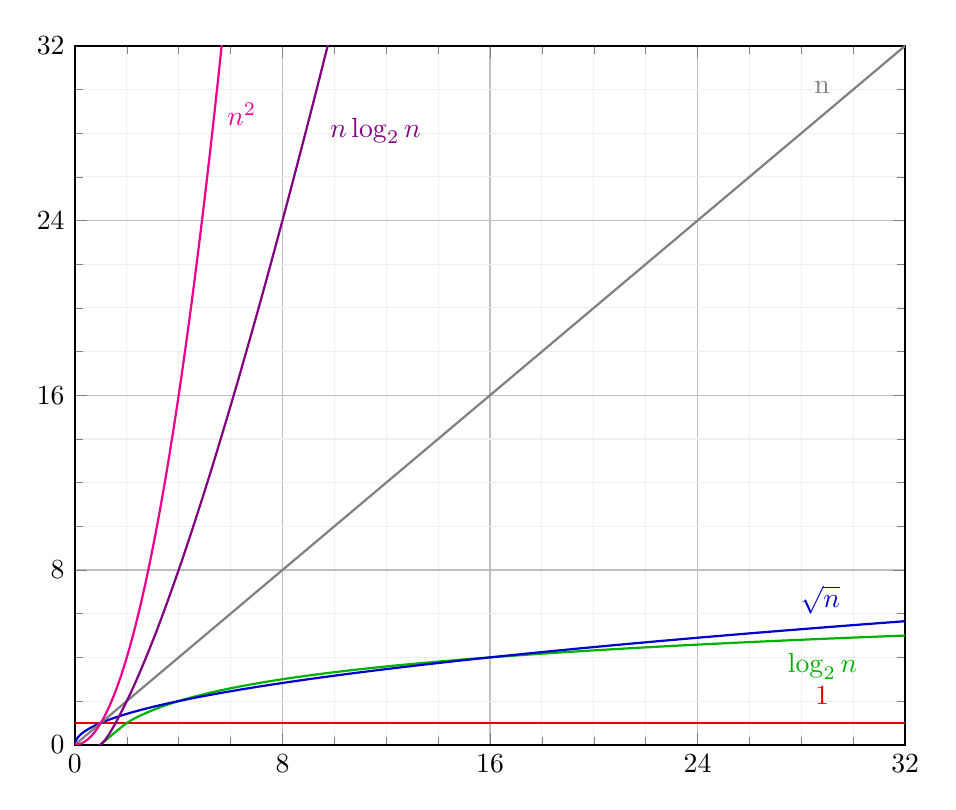
\begin{tikzpicture}
    \begin{axis}[
        width = \hsize, thick, smooth,
        domain = 0:32, xmin = 0, xmax = 32, ymin = 0, ymax = 32,
        xtick distance = 8, ytick distance = 8,
        minor tick num = 3,
        grid = both,
        major grid style = {lightgray},
        minor grid style = {lightgray!25},
        legend cell align = left,
    ]
        \addplot[red!90!black] {1}
            [yshift=1em] node [pos=0.9] {1};
        \addplot[green!70!black, samples = 32] {log2(x)}
            [yshift=-1em] node [pos=0.9] {$\log_{2}n$};
        \addplot[blue!80!black, samples = 512] {sqrt(x)}
            [yshift=1em] node [pos=0.9] {$\sqrt{n}$};
        \addplot[gray] {x}
            [yshift=1em] node [pos=0.9] {n};
        \addplot[violet, samples = 32] {x * log2(x)}
            [xshift=2em,yshift=-2em] node [pos=0.2] {$n \log_{2}n$};
        \addplot[magenta, samples = 128] {x * x}
            [xshift=1em] node [pos=0.029] {$n^2$};
    \end{axis}
\end{tikzpicture}

    \caption{Algorithmic complexity functions}
    \label{fig:algo:comp}
\end{figure}

The single most important graph in algorithmic complexity analysis is shown in
figure \ref{fig:algo:comp}.  The values of different functions are shown for
increasing positive values of the variable $n$.  These functions are used to
describe the relationship between an algorithm's resource consumption (for any
given resource of interest: number of operations/instructions, memory/disk
storage, etc.) and the size of its input.

The complexity of an algorithm is also called its \textit{order}, and the formal
definition of algorithmic complexity uses what is for that reason called
\textit{Big Omicron} or \textit{Big O} notation\footnotemark, which has the form
$f \in O(g)$.  It describes the relation between the complexity function $f$ of
an algorithm and a function $g$ according to the following principles:

\footnotetext{
    The former being a later rechristening based on Knuth's use of
    $\omega$/$\Omega$ (small omega / big omega).}

\begin{itemize}
    \item
        The notation is asymptotic: $f \in O(g)$ implies that $g$ is an upper
        bound for $f$: $f(n) <= g(n)$ for some range of values.
    \item Input sizes are always positive real numbers: $0 <= n$.
    \item
        The analysis is primarily focused on large input sizes.  Some orders may
        be faster for smaller sizes, but those are rarely the important parts of
        a program.  Therefore, $f \in O(g)$ if there is a value $n_0$ for which
        $f(n) <= g(n)$ for all $n_0 < n$, that is, even if $g(n) <= f(n)$ for
        some values of $n$, provided there is a point after which $g$ is always
        an upper bound for $f$.
    \item
        Similarly, differences between machines are critical factors but very
        difficult to analyze in the abstract, so $f \in O(g)$ if there is a
        constant $c > 0$ for which $c f(x) <= g(x)$.  That is, even if some
        constant factor influences the complexity of a specific implementation
        of an algorithm, it will become irrelevant for large input sizes and can
        be ignored.
    \item
        Usually, only the tightest bound for a function is considered.  E.g.:
        even though it is true that $f \in O(\log{n})$ implies $f \in O(n)$ (but
        not $f \in O(1)$), $O(n)$ usually means $f(n)$ is the most restrictive
        of the categories that fits the constraints above.  In general, for any
        polynomial, only its highest power of $n$ is considered, as it
        eventually dominates the value of the function.
\end{itemize}

Note that these definitions are idealistic: their intent is to formalize the
resource utilization of an algorithm as much as possible across machines of
drastically different characteristics.  As such, they model computation \emph{in
vacuo}, offering only a partial --- if very useful --- characterization
intrinsic to an algorithm, but a complete analysis must consider the
architectural components described in chapter \secref{ch:arch} and elsewhere.

Big O is part of a family of notations which describe relations between
functions.  Table \ref{tbl:algo:big_o} lists those most commonly used in
complexity analysis.

\begin{table}[ht]
    \centering
    \begin{tabular}{ccl}
        Notation & Name & Description (asymptotic) \\
        \hline
        $f(n) \in o(g(n))$ & small O / Omicron & dominated by \\
        $f(n) \in O(g(n))$ & big O / Omicron & bounded above by (see text) \\
        $f(n) \in \Theta(g(n))$ & big Theta & bounded below and above by \\
        $f(n) \sim g(n)$ & order of & equal to \\
        $f(n) \in \Omega(g(n))$ & big Omega & bounded below by \\
        $f(n) \in \omega(g(n))$ & small Omega & dominates \\
    \end{tabular}
    \caption{Family of complexity notations}
    \label{tbl:algo:big_o}
\end{table}

\textit{Constant complexity}, $f(n) = 1$, represents any function that does not
depend on the magnitude of its input.  A hash table lookup is an example of this
complexity: if the load factor of the table is managed, the number of operations
performed is independent of the number of elements in the table.  Even though
this function is usually represented by the constant $1$, from the rules above
we derive that any constant function is in the same category.

\textit{Linear complexity}, $f(n) = n$, is a function directly proportional to
its input.  Algorithms commonly operate on every element, consume one unit of
space, or otherwise perform an operation for each of their input values, making
this the most common function to describe their complexity, and a reference to
which other functions are compared.  A linear search over an array of elements
is an example of this complexity.

Different interesting subsets of these functions can be analyzed in separation
so that the scale of the graphs can be adjusted, as they quickly become wildly
divergent outside the range displayed in the graph.  Figure
\ref{fig:algo:comp_nlog_sqrt_n} compares the lower part of the original graph to
the growth of $n$, this time using a logarithmic scale.

\begin{figure}[ht]
    \centering
    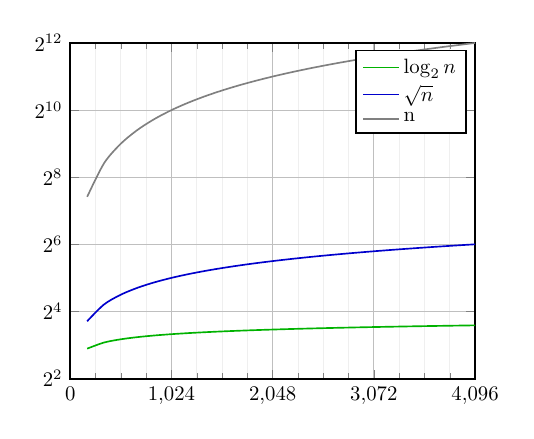
\begin{tikzpicture}[scale=0.75]
        \begin{semilogyaxis}[
            thick, smooth,
            log basis y = 2,
            domain = 0:4096, xmin = 0, xmax = 4096, ymax = 4096,
            xtick distance = 1024,
            minor tick num = 3,
            grid = both,
            major grid style = {lightgray},
            minor grid style = {lightgray!25},
            legend cell align = left,
        ]
            \addplot[green!70!black] {log2(x)};
            \addplot[blue!80!black] {sqrt(x)};
            \addplot[gray] {x};
            \legend{$\log_{2}n$, $\sqrt{n}$, n}
        \end{semilogyaxis}
    \end{tikzpicture}
    \caption{$n \log_{2}n$ vs. $\sqrt{n}$}
    \label{fig:algo:comp_nlog_sqrt_n}
\end{figure}

\textit{Logarithmic complexity} (referring as always in this section to the
logarithm base 2 unless given an explicit base), $f(n) = \log_{2}n$, is the
pattern of algorithms that reduce their domain by some constant factor in each
iteration, usually by half.  A binary search is an example of this complexity.

This is a very important function that is common of optimized algorithms which
dramatically reduces resource consumption, as the $\log_{2}$ remains a
relatively low number, very similar to a constant factor, even for very large
(in terms of numbers that computers usually deal with) values of $n$.  As an
example, the two most common word sizes currently are 32 and 64 bits.  These can
address arrays of roughly two million and ten quintillion bytes, but the
logarithm base two of those values is, obviously, 32 and 64.  This demonstrates
both that doubling the logarithm has an enormous effect on the corresponding
value of $n$ and that the logarithm is relatively small for very large values of
$n$.

\textit{Fractional power complexity} is a less common case of algorithms which
reduce their input by a fractional exponent, typically 2 --- i.e. $f(n) =
\sqrt(n)$.  A linear primality test that tests the divisibility by every number
up to the square root of its input is an example of this complexity.  Although
both $n \log_{2}n$ and $\sqrt{n}$ appear lower and very similar in the original
graph, the latter grows more quickly, as can be seen in the logarithmic scale
graph, but both stay several orders of magnitude below $n$.

\textit{Quasilinear complexity}, $f(n) = n \log_{2}n$ is also a common case of
algorithms that reduce their domain by half as in the case of logarithmic
complexity but in relation to the operations performed for each of its input
elements.  Sorting algorithms are an example of this complexity.  Although the
original graph shows this function quickly growing past the range displayed,
this class of algorithms is still considered tractable as, just like for
logarithmic complexity, the logarithm resembles a constant at larger values of
$n$.

Figure \ref{fig:algo:comp_n_nlog} shows the relationship between the functions
$n \log_{2}n$ and $n$.  While steeper, its growth is contained due to the fact
that the $\log_{2}n$ term has a relatively moderate growth, as we saw when we
analyzed logarithmic complexity.

\begin{figure}[ht]
    \centering
    \hfill
    \begin{subfigure}[h]{0.45\textwidth}
        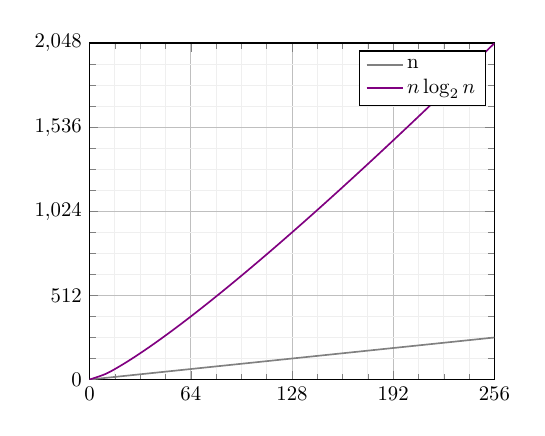
\begin{tikzpicture}[scale=0.75]
            \begin{axis}[
                thick, smooth,
                domain = 0:256, xmin = 0, xmax = 256, ymin = 0, ymax = 2048,
                xtick distance = 64, ytick distance = 512,
                minor tick num = 3,
                grid = both,
                major grid style = {lightgray},
                minor grid style = {lightgray!25},
                legend cell align = left,
            ]
                \addplot[gray] {x};
                \addplot[violet] {x * log2(x)};
                \legend{n, $n \log_{2}n$}
            \end{axis}
        \end{tikzpicture}
        \caption{n vs. $n \log_{2}n$}
        \label{fig:algo:comp_n_nlog}
    \end{subfigure}
    \hfill
    \begin{subfigure}[h]{0.45\textwidth}
        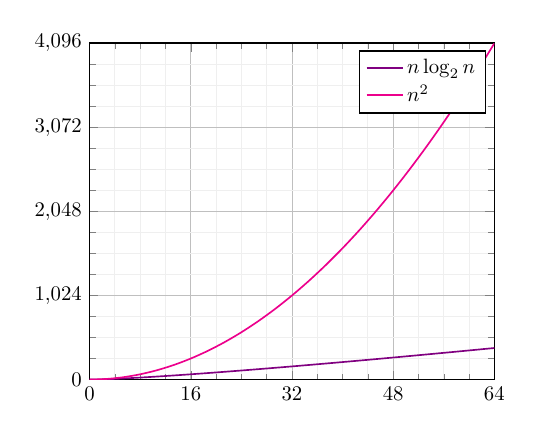
\begin{tikzpicture}[scale=0.75]
            \begin{axis}[
                thick, smooth,
                domain = 0:64, xmin = 0, xmax = 64, ymin = 0, ymax = 4096,
                xtick distance = 16, ytick distance = 1024,
                minor tick num = 3,
                grid = both,
                major grid style = {lightgray},
                minor grid style = {lightgray!25},
                legend cell align = left,
            ]
                \addplot[violet] {x * log2(x)};
                \addplot[magenta] {x * x};
                \legend{$n \log_{2}n$, $n^2$}
            \end{axis}
        \end{tikzpicture}
        \caption{$n \log_{2}n$ vs. $n^2$}
        \label{fig:algo:comp_nlog_n2}
    \end{subfigure}
    \hfill
    \caption{$n, n \log_{2}n, n^2$}
    \label{fig:algo:comp_n_nlog_n2}
\end{figure}

\textit{Polynomial complexity} describes algorithms whose complexity is defined
by a polynomial.  Quadratic complexity, $f(n) = n^2$, is its most common type,
where an algorithm performs an operation for each element of the Cartesian
product of its input.  Less optimized sorting algorithms, such as selection and
bubble sort, are examples of this complexity.

Figure \ref{fig:algo:comp_nlog_n2} shows the relationship between $n \log_{2}n$
and $n^2$.  While both are shown to rise quickly above $n$, the growth of $n^2$
is much more rapid (in a non-linear fashion) compared to $n \log_{2}n$.

\section{Sorting}

\subsection{Ordering}
\label{subsec:algo:ordering}

\begin{description}
    \item[Partial order]
        is an ordering relation which cannot be used to order all elements of a
        set.
    \item[Weak partial order]
        is a partial ordering relation which is reflexive, i.e. for relation
        $R$, $\forall x \in X, x R x$.  The \textit{less-than-or-equal} relation
        ($\leq$) is weak since $x \leq x$.
    \item[Strong partial order]
        is a partial ordering relation which is irreflexive, i.e. for relation
        $R$, $\forall x \in X, \neg(x R x)$.  The \textit{less-than} relation
        ($<$) is strong since $\neg(x < x)$.
    \item[Total order]
        is an ordering relation where every element can be classified as
        preceding or succeeding every other element.
\end{description}

\begin{aside}
    Examples of weak partial orders that occur commonly in programming are:
    \begin{itemize}
        \item
            The edges of a directed acyclic graph.  Ancestors in unrelated
            hierarchies have no relation to each other.
        \item
            The \textit{happens-before} relation in memory ordering operations
            (v.  \secrefpar{sec:conc:atomic}).  Two operations that happen
            before a third are unsequenced with respect to each other.
    \end{itemize}
\end{aside}

Note that (several) total orders can always be established for finite partial
orders:

\begin{itemize}
    \item
        A particular topological order of a directed acyclic graph establishes a
        total order from the partial order described by its edges.
    \item
        A particular sequence of operations under sequential consistency
        establishes a total order from the partial order of memory ordering
        operations.
\end{itemize}

\subsection{Equivalence}

In mathematics and computer science, two concepts are involved in determining
the fundamental relation between values of a given type: \textit{equivalence}
and \textit{equality}.  Equivalence (often represented as $\sim$ or $\equiv$) is
described mathematically as a binary relation that is:

\begin{description}
    \item[Reflexive] $x \sim x$
    \item[Symmetric] $x \sim y \implies y \sim x$
    \item[Transitive] $(x \sim y) \land (y \sim z) \implies x \sim z$
\end{description}

Any relation which satisfies these properties is an \textit{equivalence
relation}.  Equality is the canonical equivalence relation: $x$ and $y$ are
\textit{equal} iff they have the same value.  Equivalence relations are
interesting in both mathematics and computer science because they still apply to
types which may not have a strict equality relation: it is a more general
relation.

In practical terms, specifically in the context of sorting and searching
algorithms, a \textit{strict partial order} (i.e. irreflexive) is sufficient for
their implementation.  This allows these algorithms to be applied to types which
do not have a concept of equality and simplifies their interface, since a single
relation can be used for all operations instead of two.  For example, the
\texttt{std::sort} and \texttt{std::binary\_search} algorithms (to list a few)
in the C++ standard library define their semantics in terms of an equivalence
relation, for which \texttt{std::less} --- a generic version of the \texttt{<}
operator --- is the canonical implementation, establishing the following
definitions:

\begin{description}
    \item[Equality]
        \texttt{x == y}, as dictated by \texttt{operator==}
    \item[Equivalence]
        \texttt{!(x < y) \&\& !(y < x)}, as dictated by \texttt{operator<}
\end{description}

\subsection{Selection sort}

\begin{figure}[p]
    \centering
    \lstinputlisting[
        style=c++,
        firstline=7,
        caption={Selection sort},
        label={lst:algo:selection},
    ]{algo/sort/selection.cpp}
    \vspace{2\baselineskip}
    \begin{subfigure}[h]{0.3\textwidth}
    \begin{tikzpicture}[>={Stealth[round]}, text height = 0.75em]
        \matrix {
            \node (n0) [rectangle, draw] {2}; &
            \node (n1) [rectangle, draw] {1}; &
            \node (n2) [rectangle, draw] {7}; &
            \node (n3) [rectangle, draw] {5}; &
            \node (n4) [rectangle, draw] {6}; &
            \node (n5) [rectangle, draw] {0}; &
            \node (n6) [rectangle, draw] {4}; &
            \node (n7) [rectangle, draw] {3}; \\
        };
        \node (b) at ($ (n0.south west) - (0, 0.75) $) {b};
        \node (m) at ($ (n5.south west) - (0, 0.75) $) {min};
        \node (e) at ($ (n7.south east) - (0, 0.75) $) {e};
        \draw[->] (b) -- ($ (n0.south west) - (0, 0.1) $);
        \draw[->] (m) -- ($ (n5.south west) - (0, 0.1) $);
        \draw[->] (e) -- ($ (n7.south east) - (0, 0.1) $);
    \end{tikzpicture}
\end{subfigure}
\quad
\begin{subfigure}[h]{0.3\textwidth}
    \begin{tikzpicture}[>={Stealth[round]}, text height = 0.75em]
        \matrix {
            \node (n0) [rectangle, draw, fill = green!50] {0}; &
            \node (n1) [rectangle, draw] {1}; &
            \node (n2) [rectangle, draw] {7}; &
            \node (n3) [rectangle, draw] {5}; &
            \node (n4) [rectangle, draw] {6}; &
            \node (n5) [rectangle, draw] {2}; &
            \node (n6) [rectangle, draw] {4}; &
            \node (n7) [rectangle, draw] {3}; \\
        };
        \node (b) at ($ (n1.south west) - (0, 0.8) $) {b/min};
        \node (e) at ($ (n7.south east) - (0, 0.75) $) {e};
        \draw[->] (b) -- ($ (n1.south west) - (0, 0.1) $);
        \draw[->] (e) -- ($ (n7.south east) - (0, 0.1) $);
    \end{tikzpicture}
\end{subfigure}
\quad
\begin{subfigure}[h]{0.3\textwidth}
    \begin{tikzpicture}[>={Stealth[round]}, text height = 0.75em]
        \matrix {
            \node (n0) [rectangle, draw, fill = green!50] {0}; &
            \node (n1) [rectangle, draw, fill = green!50] {1}; &
            \node (n2) [rectangle, draw] {7}; &
            \node (n3) [rectangle, draw] {5}; &
            \node (n4) [rectangle, draw] {6}; &
            \node (n5) [rectangle, draw] {2}; &
            \node (n6) [rectangle, draw] {4}; &
            \node (n7) [rectangle, draw] {3}; \\
        };
        \node (b) at ($ (n2.south west) - (0, 0.75) $) {b};
        \node (m) at ($ (n5.south west) - (0, 0.75) $) {min};
        \node (e) at ($ (n7.south east) - (0, 0.75) $) {e};
        \draw[->] (b) -- ($ (n2.south west) - (0, 0.1) $);
        \draw[->] (m) -- ($ (n5.south west) - (0, 0.1) $);
        \draw[->] (e) -- ($ (n7.south east) - (0, 0.1) $);
    \end{tikzpicture}
\end{subfigure}
\\[\baselineskip]
\begin{subfigure}[h]{0.3\textwidth}
    \begin{tikzpicture}[>={Stealth[round]}, text height = 0.75em]
        \matrix {
            \node (n0) [rectangle, draw, fill = green!50] {0}; &
            \node (n1) [rectangle, draw, fill = green!50] {1}; &
            \node (n2) [rectangle, draw, fill = green!50] {2}; &
            \node (n3) [rectangle, draw] {5}; &
            \node (n4) [rectangle, draw] {6}; &
            \node (n5) [rectangle, draw] {7}; &
            \node (n6) [rectangle, draw] {4}; &
            \node (n7) [rectangle, draw] {3}; \\
        };
        \node (b) at ($ (n3.south west) - (0, 0.75) $) {b};
        \node (m) at ($ (n7.south west) - (0, 0.75) $) {min};
        \node (e) at ($ (n7.south east) - (0, 0.75) $) {e};
        \draw[->] (b) -- ($ (n3.south west) - (0, 0.1) $);
        \draw[->] (m) -- ($ (n7.south west) - (0, 0.1) $);
        \draw[->] (e) -- ($ (n7.south east) - (0, 0.1) $);
    \end{tikzpicture}
\end{subfigure}
\quad
\begin{subfigure}[h]{0.3\textwidth}
    \begin{tikzpicture}[>={Stealth[round]}, text height = 0.75em]
        \matrix {
            \node (n0) [rectangle, draw, fill = green!50] {0}; &
            \node (n1) [rectangle, draw, fill = green!50] {1}; &
            \node (n2) [rectangle, draw, fill = green!50] {2}; &
            \node (n3) [rectangle, draw, fill = green!50] {3}; &
            \node (n4) [rectangle, draw] {6}; &
            \node (n5) [rectangle, draw] {7}; &
            \node (n6) [rectangle, draw] {4}; &
            \node (n7) [rectangle, draw] {5}; \\
        };
        \node (b) at ($ (n4.south west) - (0, 0.75) $) {b};
        \node (m) at ($ (n6.south west) - (0, 0.75) $) {min};
        \node (e) at ($ (n7.south east) - (0, 0.75) $) {e};
        \draw[->] (b) -- ($ (n4.south west) - (0, 0.1) $);
        \draw[->] (m) -- ($ (n6.south west) - (0, 0.1) $);
        \draw[->] (e) -- ($ (n7.south east) - (0, 0.1) $);
    \end{tikzpicture}
\end{subfigure}
\quad
\begin{subfigure}[h]{0.3\textwidth}
    \begin{tikzpicture}[>={Stealth[round]}, text height = 0.75em]
        \matrix {
            \node (n0) [rectangle, draw, fill = green!50] {0}; &
            \node (n1) [rectangle, draw, fill = green!50] {1}; &
            \node (n2) [rectangle, draw, fill = green!50] {2}; &
            \node (n3) [rectangle, draw, fill = green!50] {3}; &
            \node (n4) [rectangle, draw, fill = green!50] {4}; &
            \node (n5) [rectangle, draw] {7}; &
            \node (n6) [rectangle, draw] {6}; &
            \node (n7) [rectangle, draw] {5}; \\
        };
        \node (b) at ($ (n5.south west) - (0, 0.75) $) {b};
        \node (m) at ($ (n7.south west) - (0, 0.75) $) {min};
        \node (e) at ($ (n7.south east) - (0, 0.75) $) {e};
        \draw[->] (b) -- ($ (n5.south west) - (0, 0.1) $);
        \draw[->] (m) -- ($ (n7.south west) - (0, 0.1) $);
        \draw[->] (e) -- ($ (n7.south east) - (0, 0.1) $);
    \end{tikzpicture}
\end{subfigure}
\\[\baselineskip]
\begin{subfigure}[h]{0.3\textwidth}
    \begin{tikzpicture}[>={Stealth[round]}, text height = 0.75em]
        \matrix {
            \node (n0) [rectangle, draw, fill = green!50] {0}; &
            \node (n1) [rectangle, draw, fill = green!50] {1}; &
            \node (n2) [rectangle, draw, fill = green!50] {2}; &
            \node (n3) [rectangle, draw, fill = green!50] {3}; &
            \node (n4) [rectangle, draw, fill = green!50] {4}; &
            \node (n5) [rectangle, draw, fill = green!50] {5}; &
            \node (n6) [rectangle, draw] {6}; &
            \node (n7) [rectangle, draw] {7}; \\
        };
        \node (b) at ($ (n6.south west) - (0, 0.8) $) {b/min};
        \node (e) at ($ (n7.south east) - (0, 0.75) $) {e};
        \draw[->] (b) -- ($ (n6.south west) - (0, 0.1) $);
        \draw[->] (e) -- ($ (n7.south east) - (0, 0.1) $);
    \end{tikzpicture}
\end{subfigure}
\quad
\begin{subfigure}[h]{0.3\textwidth}
    \begin{tikzpicture}[>={Stealth[round]}, text height = 0.75em]
        \matrix {
            \node (n0) [rectangle, draw, fill = green!50] {0}; &
            \node (n1) [rectangle, draw, fill = green!50] {1}; &
            \node (n2) [rectangle, draw, fill = green!50] {2}; &
            \node (n3) [rectangle, draw, fill = green!50] {3}; &
            \node (n4) [rectangle, draw, fill = green!50] {4}; &
            \node (n5) [rectangle, draw, fill = green!50] {5}; &
            \node (n6) [rectangle, draw, fill = green!50] {6}; &
            \node (n7) [rectangle, draw] {7}; \\
        };
        \node (b) at ($ (n7.south west) - (0.2, 0.8) $) {b/min};
        \node (e) at ($ (n7.south east) - (0, 0.75) $) {e};
        \draw[->]
            ($ (b.north) + (0.2, 0) $)
            -- ($ (n7.south west) - (0, 0.1) $);
        \draw[->] (e) -- ($ (n7.south east) - (0, 0.1) $);
    \end{tikzpicture}
\end{subfigure}
\quad
\begin{subfigure}[h]{0.3\textwidth}
    \begin{tikzpicture}[>={Stealth[round]}, text height = 0.75em]
        \matrix {
            \node (n0) [rectangle, draw, fill = green!50] {0}; &
            \node (n1) [rectangle, draw, fill = green!50] {1}; &
            \node (n2) [rectangle, draw, fill = green!50] {2}; &
            \node (n3) [rectangle, draw, fill = green!50] {3}; &
            \node (n4) [rectangle, draw, fill = green!50] {4}; &
            \node (n5) [rectangle, draw, fill = green!50] {5}; &
            \node (n6) [rectangle, draw, fill = green!50] {6}; &
            \node (n7) [rectangle, draw, fill = green!50] {7}; \\
        };
        \node (b) at ($ (n7.south east) - (0, 0.8) $) {b/e};
        \draw[->] (b) -- ($ (n7.south east) - (0, 0.1) $);
    \end{tikzpicture}
\end{subfigure}

    \caption{Selection sort}
    \label{fig:algo:selection}
\end{figure}

One of the simplest sorting algorithms is \textit{selection sort}, which works
by progressively sorting the left side of the range one element at a time
(figure \ref{fig:algo:selection}).  In each iteration, the minimum value in the
unsorted portion is found (\emph{selected}) and placed at the beginning,
increasing the size of the sorted range by one element.  When all positions of
the range have gone through this procedure, the range is sorted.

The implementation of the algorithm follows naturally from this description
(listing \ref{lst:algo:selection}).  In each iteration, the beginning of the
range is guaranteed to already be sorted.  The minimum element of the rest of
the unsorted range is found, swapped with the element at the beginning of the
range, guaranteeing that the range is now partitioned with respect to the
selected element.

\subsection{Quick sort}

\begin{figure}[p]
    \centering
    \lstinputlisting[
        style=c++,
        firstline=8,
        lastline=15,
        caption={Quick sort},
        label={lst:algo:quick},
    ]{algo/sort/quick.cpp}
    \vspace{2\baselineskip}
    \begin{subfigure}[t]{0.3\textwidth}
    \centering
    \begin{tikzpicture}[>={Stealth[round]}, text height = 0.75em]
        \matrix {
            \node (n0) [rectangle, draw] {2}; &
            \node (n1) [rectangle, draw] {1}; &
            \node (n2) [rectangle, draw] {7}; &
            \node (n3) [rectangle, draw] {5}; &
            \node (n4) [rectangle, draw] {6}; &
            \node (n5) [rectangle, draw] {0}; &
            \node (n6) [rectangle, draw] {4}; &
            \node (n7) [rectangle, draw] {3}; \\
        };
        \node (i) at ($ (n6.south west) - (0, 0.75) $) {i};
        \draw[->] (i) -- ($ (n6.south west) - (0, 0.1) $);
    \end{tikzpicture}
    \begin{tikzpicture}[>={Stealth[round]}, text height = 0.75em]
        \matrix {
            \node (n0) [rectangle, draw] {4}; &
            \node (n1) [rectangle, draw] {1}; &
            \node (n2) [rectangle, draw] {7}; &
            \node (n3) [rectangle, draw] {5}; &
            \node (n4) [rectangle, draw] {6}; &
            \node (n5) [rectangle, draw] {0}; &
            \node (n6) [rectangle, draw] {2}; &
            \node (n7) [rectangle, draw] {3}; \\
        };
        \node (b) at ($ (n0.south west) - (0, 0.75) $) {b};
        \node (i) at ($ (n6.south west) - (0, 0.75) $) {i};
        \draw[->] (b) -- ($ (n0.south west) - (0, 0.1) $);
        \draw[->] (i) -- ($ (n6.south west) - (0, 0.1) $);
    \end{tikzpicture}
    \begin{tikzpicture}[>={Stealth[round]}, text height = 0.75em]
        \matrix {
            \node (n0) [rectangle, draw] {4}; &
            \node (n1) [rectangle, draw] {1}; &
            \node (n2) [rectangle, draw] {3}; &
            \node (n3) [rectangle, draw] {2}; &
            \node (n4) [rectangle, draw] {0}; &
            \node (n5) [rectangle, draw] {6}; &
            \node (n6) [rectangle, draw] {5}; &
            \node (n7) [rectangle, draw] {7}; \\
        };
        \node (b) at ($ (n0.south west) - (0, 0.75) $) {b};
        \node (p) at ($ (n5.south west) - (0, 0.75) $) {p};
        \draw[->] (b) -- ($ (n0.south west) - (0, 0.1) $);
        \draw[->] (p) -- ($ (n5.south west) - (0, 0.1) $);
    \end{tikzpicture}
    \begin{tikzpicture}[>={Stealth[round]}, text height = 0.75em]
        \matrix {
            \node (n0) [rectangle, draw] {0}; &
            \node (n1) [rectangle, draw] {1}; &
            \node (n2) [rectangle, draw] {3}; &
            \node (n3) [rectangle, draw] {2}; &
            \node (n4) [rectangle, draw] {4}; &
            \node (n5) [rectangle, draw] {6}; &
            \node (n6) [rectangle, draw] {5}; &
            \node (n7) [rectangle, draw] {7}; \\
        };
        \node (b) at ($ (n0.south west) - (0, 0.75) $) {b};
        \node (p) at ($ (n5.south west) - (0, 0.75) $) {p};
        \draw[->] (b) -- ($ (n0.south west) - (0, 0.1) $);
        \draw[->] (p) -- ($ (n5.south west) - (0, 0.1) $);
    \end{tikzpicture}
    \begin{tikzpicture}[>={Stealth[round]}, text height = 0.75em]
        \matrix {
            \node (n0) [rectangle, draw] {0}; &
            \node (n1) [rectangle, draw] {1}; &
            \node (n2) [rectangle, draw] {3}; &
            \node (n3) [rectangle, draw] {2}; &
            \node (n4) [rectangle, draw, fill = green!50] {4}; &
            \node (n5) [rectangle, draw] {6}; &
            \node (n6) [rectangle, draw] {5}; &
            \node (n7) [rectangle, draw] {7}; \\
        };
        \node (p) at ($ (n5.south west) - (0, 0.75) $) {p};
        \draw[->] (p) -- ($ (n5.south west) - (0, 0.1) $);
    \end{tikzpicture}
    \caption{Initial bisection}
\end{subfigure}
\vrule
\begin{subfigure}[t]{0.3\textwidth}
    \centering
    \begin{tikzpicture}[>={Stealth[round]}, text height = 0.75em]
        \matrix {
            \node (n0) [rectangle, draw] {0}; &
            \node (n1) [rectangle, draw] {1}; &
            \node (n2) [rectangle, draw] {3}; &
            \node (n3) [rectangle, draw] {2}; &
            \node (n4) [rectangle, draw, fill = green!50] {\phantom{0}}; &
            \node (n5) [rectangle, draw]  {\phantom{0}}; &
            \node (n6) [rectangle, draw]  {\phantom{0}}; &
            \node (n7) [rectangle, draw]  {\phantom{0}}; \\
        };
        \node (i) at ($ (n3.south west) - (0, 0.75) $) {i};
        \draw[->] (i) -- ($ (n3.south west) - (0, 0.1) $);
        \draw[ultra thick] (n4.south west) -- (n4.north west);
    \end{tikzpicture}
    \begin{tikzpicture}[>={Stealth[round]}, text height = 0.75em]
        \matrix {
            \node (n0) [rectangle, draw] {2}; &
            \node (n1) [rectangle, draw] {1}; &
            \node (n2) [rectangle, draw] {3}; &
            \node (n3) [rectangle, draw] {0}; &
            \node (n4) [rectangle, draw, fill = green!50] {\phantom{0}}; &
            \node (n5) [rectangle, draw]  {\phantom{0}}; &
            \node (n6) [rectangle, draw]  {\phantom{0}}; &
            \node (n7) [rectangle, draw]  {\phantom{0}}; \\
        };
        \node (b) at ($ (n0.south west) - (0, 0.75) $) {b};
        \node (i) at ($ (n3.south west) - (0, 0.75) $) {i};
        \draw[->] (b) -- ($ (n0.south west) - (0, 0.1) $);
        \draw[->] (i) -- ($ (n3.south west) - (0, 0.1) $);
        \draw[ultra thick] (n4.south west) -- (n4.north west);
    \end{tikzpicture}
    \begin{tikzpicture}[>={Stealth[round]}, text height = 0.75em]
        \matrix {
            \node (n0) [rectangle, draw] {2}; &
            \node (n1) [rectangle, draw] {1}; &
            \node (n2) [rectangle, draw] {0}; &
            \node (n3) [rectangle, draw] {3}; &
            \node (n4) [rectangle, draw, fill = green!50] {\phantom{0}}; &
            \node (n5) [rectangle, draw]  {\phantom{0}}; &
            \node (n6) [rectangle, draw]  {\phantom{0}}; &
            \node (n7) [rectangle, draw]  {\phantom{0}}; \\
        };
        \node (b) at ($ (n0.south west) - (0, 0.75) $) {b};
        \node (p) at ($ (n3.south west) - (0, 0.75) $) {p};
        \draw[->] (b) -- ($ (n0.south west) - (0, 0.1) $);
        \draw[->] (p) -- ($ (n3.south west) - (0, 0.1) $);
        \draw[ultra thick] (n4.south west) -- (n4.north west);
    \end{tikzpicture}
    \begin{tikzpicture}[>={Stealth[round]}, text height = 0.75em]
        \matrix {
            \node (n0) [rectangle, draw] {0}; &
            \node (n1) [rectangle, draw] {1}; &
            \node (n2) [rectangle, draw] {2}; &
            \node (n3) [rectangle, draw] {3}; &
            \node (n4) [rectangle, draw, fill = green!50] {\phantom{0}}; &
            \node (n5) [rectangle, draw]  {\phantom{0}}; &
            \node (n6) [rectangle, draw]  {\phantom{0}}; &
            \node (n7) [rectangle, draw]  {\phantom{0}}; \\
        };
        \node (p) at ($ (n3.south west) - (0, 0.75) $) {p};
        \draw[->] (p) -- ($ (n3.south west) - (0, 0.1) $);
        \draw[ultra thick] (n4.south west) -- (n4.north west);
    \end{tikzpicture}
    \begin{tikzpicture}[>={Stealth[round]}, text height = 0.75em]
        \matrix {
            \node (n0) [rectangle, draw] {0}; &
            \node (n1) [rectangle, draw] {1}; &
            \node (n2) [rectangle, draw, fill = green!50] {2}; &
            \node (n3) [rectangle, draw, fill = green!50] {3}; &
            \node (n4) [rectangle, draw, fill = green!50] {\phantom{0}}; &
            \node (n5) [rectangle, draw]  {\phantom{0}}; &
            \node (n6) [rectangle, draw]  {\phantom{0}}; &
            \node (n7) [rectangle, draw]  {\phantom{0}}; \\
        };
        \node (p) at ($ (n3.south west) - (0, 0.75) $) {p};
        \draw[->] (p) -- ($ (n3.south west) - (0, 0.1) $);
        \draw[ultra thick] (n4.south west) -- (n4.north west);
    \end{tikzpicture}
    \begin{tikzpicture}[>={Stealth[round]}, text height = 0.75em]
        \matrix {
            \node (n0) [rectangle, draw, fill = green!50] {0}; &
            \node (n1) [rectangle, draw, fill = green!50] {1}; &
            \node (n2) [rectangle, draw, fill = green!50] {\phantom{0}}; &
            \node (n3) [rectangle, draw, fill = green!50] {\phantom{0}}; &
            \node (n4) [rectangle, draw, fill = green!50] {\phantom{0}}; &
            \node (n5) [rectangle, draw]  {\phantom{0}}; &
            \node (n6) [rectangle, draw]  {\phantom{0}}; &
            \node (n7) [rectangle, draw]  {\phantom{0}}; \\
        };
        \draw[ultra thick] (n2.south west) -- (n2.north west);
        \draw[ultra thick] (n4.south west) -- (n4.north west);
    \end{tikzpicture}
    \caption{Left recursion}
\end{subfigure}
\vrule
\begin{subfigure}[t]{0.3\textwidth}
    \centering
    \begin{tikzpicture}[>={Stealth[round]}, text height = 0.75em]
        \matrix {
            \node (n0) [rectangle, draw]  {\phantom{0}}; &
            \node (n1) [rectangle, draw]  {\phantom{0}}; &
            \node (n2) [rectangle, draw]  {\phantom{0}}; &
            \node (n3) [rectangle, draw]  {\phantom{0}}; &
            \node (n4) [rectangle, draw, fill = green!50] {\phantom{0}}; &
            \node (n5) [rectangle, draw] {6}; &
            \node (n6) [rectangle, draw] {5}; &
            \node (n7) [rectangle, draw] {7}; \\
        };
        \node (i) at ($ (n5.south west) - (0, 0.75) $) {i};
        \draw[->] (i) -- ($ (n5.south west) - (0, 0.1) $);
        \draw[ultra thick] (n5.south west) -- (n5.north west);
    \end{tikzpicture}
    \begin{tikzpicture}[>={Stealth[round]}, text height = 0.75em]
        \matrix {
            \node (n0) [rectangle, draw]  {\phantom{0}}; &
            \node (n1) [rectangle, draw]  {\phantom{0}}; &
            \node (n2) [rectangle, draw]  {\phantom{0}}; &
            \node (n3) [rectangle, draw]  {\phantom{0}}; &
            \node (n4) [rectangle, draw, fill = green!50] {\phantom{0}}; &
            \node (n5) [rectangle, draw] {6}; &
            \node (n6) [rectangle, draw] {5}; &
            \node (n7) [rectangle, draw] {7}; \\
        };
        \node (i) at ($ (n5.south west) - (0, 0.75) $) {b/i};
        \draw[->] (i) -- ($ (n5.south west) - (0, 0.1) $);
        \draw[ultra thick] (n5.south west) -- (n5.north west);
    \end{tikzpicture}
    \begin{tikzpicture}[>={Stealth[round]}, text height = 0.75em]
        \matrix {
            \node (n0) [rectangle, draw]  {\phantom{0}}; &
            \node (n1) [rectangle, draw]  {\phantom{0}}; &
            \node (n2) [rectangle, draw]  {\phantom{0}}; &
            \node (n3) [rectangle, draw]  {\phantom{0}}; &
            \node (n4) [rectangle, draw, fill = green!50] {\phantom{0}}; &
            \node (n5) [rectangle, draw] {6}; &
            \node (n6) [rectangle, draw] {5}; &
            \node (n7) [rectangle, draw] {7}; \\
        };
        \node (p) at ($ (n7.south west) - (0, 0.75) $) {p};
        \draw[->] (p) -- ($ (n7.south west) - (0, 0.1) $);
        \draw[ultra thick] (n5.south west) -- (n5.north west);
    \end{tikzpicture}
    \begin{tikzpicture}[>={Stealth[round]}, text height = 0.75em]
        \matrix {
            \node (n0) [rectangle, draw]  {\phantom{0}}; &
            \node (n1) [rectangle, draw]  {\phantom{0}}; &
            \node (n2) [rectangle, draw]  {\phantom{0}}; &
            \node (n3) [rectangle, draw]  {\phantom{0}}; &
            \node (n4) [rectangle, draw, fill = green!50] {\phantom{0}}; &
            \node (n5) [rectangle, draw] {5}; &
            \node (n6) [rectangle, draw, fill = green!50] {6}; &
            \node (n7) [rectangle, draw] {7}; \\
        };
        \node (p) at ($ (n7.south west) - (0, 0.75) $) {p};
        \draw[->] (p) -- ($ (n7.south west) - (0, 0.1) $);
        \draw[ultra thick] (n5.south west) -- (n5.north west);
    \end{tikzpicture}
    \begin{tikzpicture}[>={Stealth[round]}, text height = 0.75em]
        \matrix {
            \node (n0) [rectangle, draw]  {\phantom{0}}; &
            \node (n1) [rectangle, draw]  {\phantom{0}}; &
            \node (n2) [rectangle, draw]  {\phantom{0}}; &
            \node (n3) [rectangle, draw]  {\phantom{0}}; &
            \node (n4) [rectangle, draw, fill = green!50] {\phantom{0}}; &
            \node (n5) [rectangle, draw] {5}; &
            \node (n6) [rectangle, draw, fill = green!50] {6}; &
            \node (n7) [rectangle, draw] {7}; \\
        };
        \node (p) at ($ (n7.south west) - (0, 0.75) $) {p};
        \draw[->] (p) -- ($ (n7.south west) - (0, 0.1) $);
        \draw[ultra thick] (n5.south west) -- (n5.north west);
    \end{tikzpicture}
    \begin{tikzpicture}[>={Stealth[round]}, text height = 0.75em]
        \matrix {
            \node (n0) [rectangle, draw]  {\phantom{0}}; &
            \node (n1) [rectangle, draw]  {\phantom{0}}; &
            \node (n2) [rectangle, draw]  {\phantom{0}}; &
            \node (n3) [rectangle, draw]  {\phantom{0}}; &
            \node (n4) [rectangle, draw, fill = green!50] {\phantom{0}}; &
            \node (n5) [rectangle, draw, fill = green!50] {5}; &
            \node (n6) [rectangle, draw, fill = green!50] {6}; &
            \node (n7) [rectangle, draw, fill = green!50] {7}; \\
        };
        \draw[ultra thick] (n5.south west) -- (n5.north west);
        \draw[ultra thick] (n6.south west) -- (n6.north west);
        \draw[ultra thick] (n7.south west) -- (n7.north west);
    \end{tikzpicture}
    \caption{Right recursion}
\end{subfigure}
\\
\vspace{1.5\baselineskip}
\begin{subfigure}[t]{0.3\textwidth}
    \centering
    \begin{tikzpicture}[>={Stealth[round]}, text height = 0.75em]
        \matrix {
            \node (n0) [rectangle, draw, fill = green!50] {0}; &
            \node (n1) [rectangle, draw, fill = green!50] {1}; &
            \node (n2) [rectangle, draw, fill = green!50] {2}; &
            \node (n3) [rectangle, draw, fill = green!50] {3}; &
            \node (n4) [rectangle, draw, fill = green!50] {4}; &
            \node (n5) [rectangle, draw, fill = green!50] {5}; &
            \node (n6) [rectangle, draw, fill = green!50] {6}; &
            \node (n7) [rectangle, draw, fill = green!50] {7}; \\
        };
    \end{tikzpicture}
    \caption{Sorted result}
\end{subfigure}

    \caption{Quick sort}
    \label{fig:algo:quick}
\end{figure}

Quick sort\footnote{\cite{Hoare1962}} is based on the familiar method of binary
recursion.  The range to be sorted is partitioned in two based on whether
elements are lesser or greater than a reference element (the \textit{pivot}).
This places that element at its correct position in the sorted range.  The
process is then repeated for the sub-ranges on its left and right.  Recursion
stops at the base case of a single element, which is by definition already
sorted.  Figure \ref{fig:algo:quick} illustrates each step in this
process\footnotemark, and listing \ref{lst:algo:quick} shows the implementation.
It is very concise since most of the actual work is done by utility functions.
The complexity of the entire operation is directly dependent on the partitioning
done in each recursive step:

\footnotetext{
    Conceptually, at least.  The implementation uses the empty range as the base
    case for simplicity.  In practice, sorting small arrays is done more
    efficiently with other methods, so implementations choose a critical length
    below which sorting is deferred to a different algorithm.
}

\begin{itemize}
    \item Ordering elements around the pivot is an $O(n)$ operation.
    \item
        The second factor depends on the point at which the range is
        partitioned:
        \begin{itemize}
            \item
                A perfect bisection reduces the range in half, thus sorting the
                entire range in $\log_2 n$ steps and yielding an overall
                complexity of $O(n \log n)$.
            \item
                Partitions which diverge from the median value increase the
                number of recursive steps.  The worst-case complexity is thus
                $O(n^2)$, which happens when the range is reduced by a single
                element in each step.
        \end{itemize}
\end{itemize}

Despite its worst-case complexity, carefully-chosen pivot selection and
partitioning methods\footnote{\cite{Bentley1993}} can result in very efficient
implementations.  Together with the fact that sorting is done in-place and
requires only a less-than operator makes it a common choice for standard
non-stable sorting functions.  This is the origin of the name of the
\texttt{qsort} function in the C standard library.

\section{Binary search}
\label{sec:algo:bsearch}

Even though it may seem that examining every item in an array is required to
determine whether an element is present in it, the process can be significantly
improved, provided that the sequence is sorted in advance.  In that case, vast
portions of it can be eliminated with each comparison, a technique generally
known as \textit{divide-and-conquer}.  This provides a great advantage in cases
where searches are much more common than modifications to the sequence of items
--- i.e. where the cost of sorting the sequence can be paid once and the result
used by a number of searches.

The critical aspect of the implementation is to examine the \emph{middle}
element of the sequence.  If it is \emph{less} than the desired value, the
entire lower half of the array can be ignored.  Conversely, if it is
\emph{greater} than the desired value, the entire upper half can be ignored.
The process is then repeated until the result is found or the range becomes
empty.

Due to this process of halving in each iteration, this algorithm is called a
\textit{binary search}, and is a dramatic improvement over a linear search.  For
a sequence of $2^n$ elements, a linear search has to examine at worst all $2^n$
elements.  A binary search will reduce the search space to $2^{n-1}$ after the
first iteration, $2^{n-2}$ after the second, and so on, until it reaches $2^0 =
1$, resulting in only $n+1$ iterations\footnotemark.

\footnotetext{
    Section \secref{sec:algo:comp} explores the implications of this difference
    in much more detail.}

Figure \ref{fig:algo:bsearch0} shows one execution of a binary search on the
array \texttt{[0, 1, 2, 3, 5, 6, 7, 8]} for the value \texttt{3}.  The first
middle value is \texttt{5}, which is greater than the desired value, so the
upper portion of the array is eliminated.  The next middle value is \texttt{2},
which is less than the desired value, so the lower portion of the remaining
range is eliminated.  The last middle value is \texttt{3}, which is the desired
value, so the search ends.  Figure \ref{fig:algo:bsearch1} shows the search on
the same array for the value \texttt{4}, which is similar up to the last step,
where \texttt{x} is greater than \texttt{*m}, so the range becomes empty.

\begin{figure}[p]
    \centering
    \lstinputlisting[
        style=c,
        firstline=8,
        caption={Binary search},
        label={lst:algo:bsearch},
    ]{algo/bsearch.c}
    \vspace{2\baselineskip}
    \begin{subfigure}[h]{\textwidth}
        \centering
        \begin{subfigure}[h]{0.3\textwidth}
    \begin{tikzpicture}[>={Stealth[round]}, text height = 0.75em]
        \matrix {
            \node (n0) [rectangle, draw] {0}; &
            \node (n1) [rectangle, draw] {1}; &
            \node (n2) [rectangle, draw] {2}; &
            \node (n3) [rectangle, draw] {3}; &
            \node (n4) [rectangle, draw] {5}; &
            \node (n5) [rectangle, draw] {6}; &
            \node (n6) [rectangle, draw] {7}; &
            \node (n7) [rectangle, draw] {8}; \\
        };
        \node (b) at ($ (n0.south west) - (0, 0.75) $) {b};
        \node (m) at ($ (n4.south west) - (0, 0.75) $) {m};
        \node (e) at ($ (n7.south east) - (0, 0.75) $) {e};
        \draw[->] (b) -- ($ (n0.south west) - (0, 0.1) $);
        \draw[->] (m) -- ($ (n4.south west) - (0, 0.1) $);
        \draw[->] (e) -- ($ (n7.south east) - (0, 0.1) $);
    \end{tikzpicture}
\end{subfigure}
\quad
\begin{subfigure}[h]{0.3\textwidth}
    \begin{tikzpicture}[>={Stealth[round]}, text height = 0.75em]
        \matrix {
            \node (n0) [rectangle, draw] {0}; &
            \node (n1) [rectangle, draw] {1}; &
            \node (n2) [rectangle, draw] {2}; &
            \node (n3) [rectangle, draw] {3}; &
            \node (n4) [rectangle, draw] {5}; &
            \node (n5) [rectangle, draw] {6}; &
            \node (n6) [rectangle, draw] {7}; &
            \node (n7) [rectangle, draw] {8}; \\
        };
        \node (b) at ($ (n0.south west) - (0, 0.75) $) {b};
        \node (m) at ($ (n2.south west) - (0, 0.75) $) {m};
        \node (e) at ($ (n4.south west) - (0, 0.75) $) {e};
        \draw[->] (b) -- ($ (n0.south west) - (0, 0.1) $);
        \draw[->] (m) -- ($ (n2.south west) - (0, 0.1) $);
        \draw[->] (e) -- ($ (n4.south west) - (0, 0.1) $);
    \end{tikzpicture}
\end{subfigure}
\quad
\begin{subfigure}[h]{0.3\textwidth}
    \begin{tikzpicture}[>={Stealth[round]}, text height = 0.75em]
        \matrix {
            \node (n0) [rectangle, draw] {0}; &
            \node (n1) [rectangle, draw] {1}; &
            \node (n2) [rectangle, draw] {2}; &
            \node (n3) [rectangle, draw] {3}; &
            \node (n4) [rectangle, draw] {5}; &
            \node (n5) [rectangle, draw] {6}; &
            \node (n6) [rectangle, draw] {7}; &
            \node (n7) [rectangle, draw] {8}; \\
        };
        \node (b) at ($ (n3.south west) - (0, 0.75) $) {b};
        \node (e) at ($ (n4.south west) - (0, 0.75) $) {e};
        \draw[->] (b) -- ($ (n3.south west) - (0, 0.1) $);
        \draw[->] (e) -- ($ (n4.south west) - (0, 0.1) $);
    \end{tikzpicture}
\end{subfigure}

        \caption{\texttt{bsearch(3, b, e)}}
        \label{fig:algo:bsearch0}
    \end{subfigure}
    \\[\baselineskip]
    \begin{subfigure}[h]{\textwidth}
        \centering
        \begin{subfigure}[h]{0.3\textwidth}
    \begin{tikzpicture}[>={Stealth[round]}, text height = 0.75em]
        \matrix {
            \node (n0) [rectangle, draw] {0}; &
            \node (n1) [rectangle, draw] {1}; &
            \node (n2) [rectangle, draw] {2}; &
            \node (n3) [rectangle, draw] {3}; &
            \node (n4) [rectangle, draw] {5}; &
            \node (n5) [rectangle, draw] {6}; &
            \node (n6) [rectangle, draw] {7}; &
            \node (n7) [rectangle, draw] {8}; \\
        };
        \node (b) at ($ (n0.south west) - (0, 0.75) $) {b};
        \node (m) at ($ (n4.south west) - (0, 0.75) $) {m};
        \node (e) at ($ (n7.south east) - (0, 0.75) $) {e};
        \draw[->] (b) -- ($ (n0.south west) - (0, 0.1) $);
        \draw[->] (m) -- ($ (n4.south west) - (0, 0.1) $);
        \draw[->] (e) -- ($ (n7.south east) - (0, 0.1) $);
    \end{tikzpicture}
\end{subfigure}
\ldots \qquad
\begin{subfigure}[h]{0.3\textwidth}
    \begin{tikzpicture}[>={Stealth[round]}, text height = 0.75em]
        \matrix {
            \node (n0) [rectangle, draw] {0}; &
            \node (n1) [rectangle, draw] {1}; &
            \node (n2) [rectangle, draw] {2}; &
            \node (n3) [rectangle, draw] {3}; &
            \node (n4) [rectangle, draw] {5}; &
            \node (n5) [rectangle, draw] {6}; &
            \node (n6) [rectangle, draw] {7}; &
            \node (n7) [rectangle, draw] {8}; \\
        };
        \node (b) at ($ (n3.south west) - (0.1, 0.8) $) {b/m};
        \node (e) at ($ (n4.south west) - (0, 0.75) $) {e};
        \draw[->]
            ($ (b.north) + (0.1, 0) $)
            -- ($ (n3.south west) - (0, 0.1) $);
        \draw[->] (e) -- ($ (n4.south west) - (0, 0.1) $);
    \end{tikzpicture}
\end{subfigure}
\begin{subfigure}[h]{0.3\textwidth}
    \begin{tikzpicture}[>={Stealth[round]}, text height = 0.75em]
        \matrix {
            \node (n0) [rectangle, draw] {0}; &
            \node (n1) [rectangle, draw] {1}; &
            \node (n2) [rectangle, draw] {2}; &
            \node (n3) [rectangle, draw] {3}; &
            \node (n4) [rectangle, draw] {5}; &
            \node (n5) [rectangle, draw] {6}; &
            \node (n6) [rectangle, draw] {7}; &
            \node (n7) [rectangle, draw] {8}; \\
        };
        \node (b) at ($ (n4.south west) - (0, 0.75) $) {b/e};
        \draw[->] (b) -- ($ (n4.south west) - (0, 0.1) $);
    \end{tikzpicture}
\end{subfigure}

        \caption{\texttt{bsearch(4, b, e)}}
        \label{fig:algo:bsearch1}
    \end{subfigure}
    \caption{Binary search}
\end{figure}

Listing \ref{lst:algo:bsearch} shows the complete implementation.  It starts by
establishing the function preconditions and the loop termination condition.  The
inputs will be the value \texttt{x} to search for and the half-open interval
$\texttt{[b, e)}$ delimiting the sorted range.  The terminating condition as
described previously is that the range being examined becomes empty.  The
assertions after the loop are the same as the ones inside it, as will be
described next.

\lstinputlisting
    [style=c,linerange=8-11,belowskip=0pt]
    {algo/bsearch.c}
\begin{lstlisting}[aboveskip=0pt,belowskip=0pt]
        // ...
\end{lstlisting}
\lstinputlisting
    [style=c,linerange=24-30,aboveskip=0pt]
    {algo/bsearch.c}

The loop body starts with the invariants:

\lstinputlisting
    [style=c,linerange=12-15]
    {algo/bsearch.c}

\vspace{-\baselineskip}
\begin{itemize}
    \item
        Any reduced range should be within the bounds of the original and in the
        correct sequence.
    \item
        As the input range is repeatedly reduced, we guarantee \texttt{x} is not
        in any of the eliminated regions --- those now outside $\texttt{[b, e)}$.
    \item
        As \texttt{b} is moved right, it should always delimit elements that are
        less than \texttt{x}.
    \item
        Similarly, as \texttt{e} is moved left, it should always delimit
        elements that are greater than \texttt{x}.
\end{itemize}

From these and the loop termination condition that \texttt{b == e}, the
following inferences can be made about the value of \texttt{b} at the bottom of
the function:

\begin{itemize}
    \item
        $ib = ie \ \implies \ x \notin [ib, ie)$
        \begin{itemize}
            \item \texttt{x} cannot be in the range since it is empty
        \end{itemize}
    \item
        $b = ib \ \implies \ x \notin [ib, ie)$
        \begin{itemize}
            \item $x < *e \ \implies \ x < *ib$
            \item
                \texttt{x} cannot be in a sorted range if it is less than the
                first element
        \end{itemize}
    \item
        $e = ie \ \implies \ x \notin [ib, ie)$
        \begin{itemize}
            \item $b[-1] < x \ \implies e[-1] < x$
            \item
                \texttt{x} cannot be in a sorted range if the last element is
                less than it
        \end{itemize}
    \item
        otherwise $\implies \ x \notin [ib, ie)$
        \begin{itemize}
            \item $x < *e \ \implies \ x < *b$
            \item $b[-1] < x$
            \item
                \texttt{x} cannot be in a sorted range if $b[-1] < x$ and $x <
                b[0]$
        \end{itemize}
\end{itemize}

That is, as long as the invariants are maintained, exiting the loop means
\texttt{x} is not contained in the range.  This is reflected in the assertions
at the bottom of the function.  The implementation of the loop begins by
determining the middle element of the range.  This is done by computing its
length and using integer division to halve it while rounding down.\footnotemark.

\footnotetext{
    The difference is first converted to an unsigned value, since we know it is
    positive, so that the division by a power of two can be translated to a few
    simple bitwise operations.  Integer division rounds values towards zero,
    while division using shifts rounds towards negative infinity.  Converting a
    value to unsigned eliminates special cases in the generated machine code
    since those two cases have the same outcome for positive values.}

\lstinputlisting[style=c,linerange=16-17]{algo/bsearch.c}

Next, the middle value is compared to \texttt{x}: if it is equal, the value has
been found\footnotemark.  Otherwise, the search range is modified according to
the rules described previously.

\footnotetext{See exercise \ref{ex:algo:bsearch_bound}}

\lstinputlisting[style=c,linerange=18-23]{algo/bsearch.c}

We can observe that the invariants are preserved in both branches that advance
to the next iteration:

\begin{multicols}{2}
    \texttt{*m < x}
    \begin{align*}
        ib \leq b' & \impliedby
        \begin{cases}
            b' = m \\
            ib \leq b \\
            b \leq m \\
        \end{cases}
        \\
        b' \leq ie & \impliedby
        \begin{cases}
            b' = m + 1 \\
            m  < e \\
            e \leq ie \\
        \end{cases}
        \\
        b'[-1] < x & \impliedby
        \begin{cases}
            b' = m + 1 \\
            *m < x \\
        \end{cases}
    \end{align*}
    \\
    \columnbreak
    \\
    \texttt{*m > x}
    \begin{align*}
        ib \leq e' & \impliedby
        \begin{cases}
            e' = m \\
            ib \leq b \\
            b \leq m \\
        \end{cases}
        \\
        e' \leq ie & \impliedby
        \begin{cases}
            e' = m \\
            m < e \\
        \end{cases}
        \\
        x < *e' & \impliedby
        \begin{cases}
            e' = m \\
            *m \neq x \\
            x < *m \\
        \end{cases}
    \end{align*}
\end{multicols}

\subsection{Exercises}

\begin{enumerate}[label*=\arabic*.]
    \item
        \label{ex:algo:bsearch_middle}
        Prove that the expression \texttt{m = b + (e - b) / 2} correctly
        calculates the middle element of a range.
    \item
        \label{ex:algo:bsearch_overflow}
        A more common mathematical definition of the middle element would be
        \texttt{m = (b + e) / 2}.  Could that be used in our implementation of
        binary search?  Prove the answer and give examples.
    \item
        \label{ex:algo:bsearch_bound}
        Our version of binary search works and is significantly faster than
        linear search, but it performs two comparisons per iteration.  A
        closely-related fact is that it will return on the first element that is
        found to be equal to the input.

        Often, the range can have duplicate values and it is desired to find
        either the first position where a value occurs or the position after its
        last occurrence, e.g. to find the place where a new element should be
        inserted to keep the range sorted.  These two algorithms are called
        lower and upper bound.  More specifically, lower bound returns the
        position that partitions the range into elements that are \texttt{< x},
        while upper bound returns the position that partitions the range into
        elements that are \texttt{> v}.  For the array \texttt{[0, 1, 3, 3, 3,
        5, 6]}, the lower bound for value \texttt{3} is position \texttt{2},
        while the upper bound is position \texttt{5}.  These are the same
        results for the lower bound for value \texttt{2} and the upper bound for
        value \texttt{4}.

        Implement both versions and then rewrite the \texttt{binary\_search}
        function in terms of \texttt{lower\-\_bound}, all with suitable
        invariants.

        \begin{lstlisting}[style=c]
        int *lower_bound(int x, int *b, int *e);
        int *upper_bound(int x, int *b, int *e);
        \end{lstlisting}
\end{enumerate}

\chapter{Data structures}
\label{ch:struct}
\section{Allocation}

Two main dynamic allocation strategies are common in software:

\begin{itemize}
    \item
        Objects are independent entities and given a dedicated region of memory
        specially allocated to store them.  This is the pattern often found in
        dynamic, high-level languages, where even primitive objects are
        \textit{boxed}, i.e. have their own distinct allocation.

        In compound structures composed of multiple fields, each value is simply
        a \textit{reference} to its sub-objects, which also have their own
        dedicated allocation.  Object construction in these languages is often
        indivisible from memory allocation, as shown in listing
        \ref{lst:struct:alloc_dedicated}.
    \item
        Lower-level languages such as C and C++ offer more control over the
        memory layout of objects.  Pointers and dynamic memory allocation
        primitives/functions can still be used to implement the previous
        pattern, but often objects are \textit{embedded} in others.

        An object --- a \texttt{struct} in C --- is the concatenation of all of
        its constituent fields\footnotemark.  Memory allocation and object
        construction are usually two distinct operations, as shown in listing
        \ref{lst:struct:alloc_embedded}.
\end{itemize}

\footnotetext{Ignoring for the moment field padding and alignment.}

Each of these allocation strategies has advantages and disadvantages.  Boxed
objects put pressure on the memory allocator and can waste memory space.  Every
variable/member access is indirect, potentially to memory locations which are
distant from each other, reducing cache efficiency.  Copying this type of object
is usually only a \textit{shallow} copy: references to sub-objects are simply
copied and continue to point to the same place.  This can cause problems when
both the original object and the copy are used in a way which expects
independent objects.  In contrast, the location in memory of boxed objects is
often stable, reducing the risk of invalid memory accesses due to relocation.

Conversely, embedded objects are very fast and compact, since a single block of
memory (either on the stack or the heap) is used to store them.  This block can
also be loaded completely in one or more cache lines, making accesses very
efficient.  Copying embedded objects (either via \ident{memcpy} in C or a copy
constructor/assignment in C++) is a \textit{deep} copy: the resulting copy is
completely independent of the original.

\begin{figure}[p]
    \lstinputlisting[
        style=c,
        caption={Structure allocation (dedicated)},
        label={lst:struct:alloc_dedicated},
        firstline=5,
    ]{struct/alloc/dedicated.c}
    \lstinputlisting[
        style=c,
        caption={Structure allocation (embedded)},
        label={lst:struct:alloc_embedded},
        firstline=5,
    ]{struct/alloc/embedded.c}
\end{figure}

\subsection{Data headers}

The complete control over memory allocation offered by the second strategy
allows other patterns to be used.  A common one is to associate extra
information with an allocation: a memory allocator may store tracking
information, a linked list may store previous/next pointers, an array of items
may store its length, etc.  A single memory block can be used both for the
contained object and its associated information.

\subsubsection{\ident{array}}

Listing \ref{lst:struct:header} shows an implementation of the latter example:
an array of bytes (or string) which stores information about the items as a
header prepended to the memory block.  The client interface deals solely with a
\texttt{char*} which points directly to the data block.  The implementation,
however, actually allocates an object of type \texttt{struct array} which stores
additional information about the object --- the size and some arbitrary set of
flags in this case.  \ident{array_alloc} allocates a single block of memory
containing both the header and the client data.  This header is easily
retrievable from the pointer returned to the client via the use of simple
pointer arithmetic, as demonstrated in \ident{array_size}, which uses the header
information.  \ident{array_destroy} uses the same calculation to pass the
correct pointer to \texttt{free} --- which likely uses a similar technique
internally for its allocation tracking data.

\begin{figure}[ht]
    \lstinputlisting[
        style=c,
        label={lst:struct:header},
        caption={Memory block header},
        firstline=10,
    ]{struct/alloc/header.c}
\end{figure}
\vspace{-\baselineskip}

\begin{aside}
    This structure uses the C99 \textit{flexible array member} syntax.
    \texttt{data} does not occupy any actual space in the object (as
    demonstrated by the \ident{static_assert}): it is simply convenient syntax
    which gives direct access to a data block of undetermined size appended to
    the object.  Using this syntax has several advantages over other methods
    (such as declaring it as an array of one element\footnotemark):
    \begin{itemize}
        \item
            \texttt{sizeof} accurately reports the size of the \texttt{struct}
            --- it does not include the array.
        \item
            It is not possible to use \texttt{sizeof} with the array member, it
            is considered as having an incomplete type.  This prevents the
            accidental use in an attempt to incorrectly calculate the size of
            the array.
        \item
            Structures with trailing flexible array members cannot be placed in
            the middle of other \texttt{struct}s or in arrays.
    \end{itemize}
    Prior to C99, some compilers (such as GCC) supported declaring an array of
    zero elements as an extension, with similar (but inferior) semantics.
\end{aside}

\footnotetext{
    Section \secref{sec:c:ub} shows an example of how mistakes in this case can
    be subtle and catastrophic.}

\subsubsection{\ident{sockaddr}}

One particular use of this pattern is in indicating that a structure is expected
to be ``extended'' by other structure types\footnotemark.  One classical example
is the Unix/POSIX \ident{struct sockaddr}.  Networking sockets of all types are
created uniformly via \ident{socket(2)}, server sockets are all bound to an
address via \ident{bind(2)}, client sockets are all connected to servers via
\ident{connect(2)}, etc.  Each networking protocol, however, has its own address
structure, called an \textit{address family} in the POSIX standard, and each
family has a different format:

\footnotetext{V. \secref{sec:c++:oop} for a complete discussion of inheritance.}

\begin{itemize}
    \item Unix-domain sockets are bound to a local path on the file system.
    \item IPv4 sockets are bound to an address and a port.
    \item
        IPv6 sockets are also bound to an address/port, but use a different
        address format.
    \item etc.
\end{itemize}

In order to support all address types, system calls receive their socket address
parameter using the following pattern:

\begin{lstlisting}[style=c]
int bind(int socket, const struct sockaddr *address, socklen_t address_len);
\end{lstlisting}

One possible definition of the types involved is shown in listing
\ref{lst:struct:sockaddr}.  \ident{struct sockaddr} is the ``base'' type: its
\ident{sa_family_t} member is an unsigned integer type --- in this way, the
structure can be conceptualized as a discriminated \ident{union} type.  The
trailing array member \ident{sa_data} indicates that extra data are placed at
the end of the object, and that the size of the structure can vary (similarly to
the one in the previous example).  For each address type, a derivative of this
structure exists, some of which are also shown in the listing.

\begin{figure}[ht]
    \centering
    \begin{subfigure}[t]{0.45\textwidth}
        \begin{lstlisting}[style=c]
struct sockaddr {
    sa_family_t sa_family;
    char sa_data[];
};

struct sockaddr_storage {
    sa_family_t ss_family;
    char ss_padding[/*...*/];
    ss_aligntype ss_align;
};
        \end{lstlisting}
    \end{subfigure}
    \begin{subfigure}[t]{0.4\textwidth}
        \begin{lstlisting}[style=c]
struct sockaddr_un {
    sa_family_t sun_family;
    char sun_path[108];
};

struct sockaddr_in {
    sa_family_t sin_family;
    u16 sin_port;
    struct in_addr sin_addr;
    char sin_pad[/*...*/];
};

struct sockaddr_in6 {
    sa_family_t sin6_family;
    u16 sin6_port;
    u32 sin6_flowinfo;
    struct in6_addr sin6_addr;
    u32 sin6_scope_id;
};
        \end{lstlisting}
    \end{subfigure}
    \captionof{lstlisting}{\ident{struct sockaddr}}
    \label{lst:struct:sockaddr}
\end{figure}

This collection of types allows socket addresses to have several different
formats.  Clients create an object of one of the specific address types and cast
them to \ident{struct sockaddr} as the \ident{address} parameter of system
calls.  Similarly, \ident{address_len}, actual size of the structure, is known
to them.  On the other side of the call, system calls can inspect
\texttt{address->sa\_family} to detect the address type and then cast the
pointer to the appropriate, derived type.  This is valid since all structures
have a common prefix.  \ident{sockaddr_storage} can be used as generic storage
for any of the derived types: its members are defined such that it will have the
correct size and alignment to satisfy all types.

\section{Linked lists}

Linked lists are a simple data structure which consist of a sequence of elements
and the connections between them (\textit{links}).  This contrasts with arrays,
which contain just the elements themselves, where the order is implicit in the
fact that elements are laid out sequentially in memory\footnotemark.  Even so,
the underlying storage for the elements is immaterial: the definition of the
data structure is only concerned with how elements are connected to each other.

\footnotetext{
    Subject to alignment and padding requirements, but still extrinsic and
    independent of the contents of each element.}

\subsection{Singly linked list}

The simplest possible implementation of a linked list is shown in figure
\ref{fig:struct:array_list0}.  A fixed-size array is used to store the elements
(separated by solid lines), where each is some data and the index of the next
element (denoted with arrows).  The iteration process starts at the list
\textit{head}, denoted by the arrow starting on the left.  After an element is
processed, the next element is obtained by adding the element's ``next'' index
to the list head.  A special index value denotes the last element, the list
\textit{tail}.  Iteration stops after this element is processed.

\begin{figure}[ht]
    \centering
    \begin{tikzpicture}[
        rectangle/.style={minimum height = 2em},
        rectangle split draw splits = false,
    ]
        \matrix {
            \node (n0) [lnode] {~ \nodepart{two} 1}; &
            \node (n1) [lnode] {~ \nodepart{two} 2}; &
            \node (n2) [lnode] {~ \nodepart{two} 3}; &
            \node (n3) [lnode] {~ \nodepart{two} 4}; &
            \node (n4) [lnode] {~ \nodepart{two} 5}; &
            \node (n5) [lnode] {~ \nodepart{two} 6}; &
            \node (n6) [lnode] {~ \nodepart{two} 7}; &
            \node (n7) [lnode] {\phantom{7}}; \\
            \node {0}; & \node {1}; & \node {2}; & \node {3}; &
            \node {4}; & \node {5}; & \node {6}; & \node {7}; \\
        };
        \foreach \n in {n0, n1, n2, n3, n4, n5, n6, n7} {
            \draw[dashed]
                ($ (\n.north west)!0.5!(\n.north east) $)
                -- ($ (\n.south west)!0.5!(\n.south east) $);
        }
        \draw ($ (n0) - (1, 0) $) edge[->] (n0.west);
        \foreach \n/\m in {n0/n1, n1/n2, n2/n3, n3/n4, n4/n5, n5/n6, n6/n7} {
            \draw
                ($ (\n.north west)!0.75!(\n.north east) $)
                -- +(0, 0.25)
                -- ($ (\m.north west)!0.5!(\m.north east) + (0, 0.25) $)
                edge[->] +(0, -0.25);
        }
    \end{tikzpicture}
    \caption{Array as linked list}
    \label{fig:struct:array_list0}
\end{figure}

Because there is a single link in each element that points forward to the next
element, this type of structure is called a \textit{singly linked list} or
\textit{forward list}.  One advantage they have over arrays becomes apparent
when elements are added and/or removed.  When these operations are performed in
an array in any position that is not the last, elements must be shift either up
or down to make or fill the space for the target position.  In a linked list,
these operations simply manipulate the links between elements.

Figure \ref{fig:struct:array_list1} shows the same list after a few of these
operations.  The sequence of elements is now \texttt{0, 2, 4, 1, 5, 6} even
though they all retain their previous location in memory.

\begin{figure}[ht]
    \centering
    \begin{tikzpicture}[
        rectangle/.style={minimum height = 2em},
        rectangle split draw splits = false,
    ]
        \matrix {
            \node (n0) [lnode] {~ \nodepart{two} 2}; &
            \node (n1) [lnode] {~ \nodepart{two} 6}; &
            \node (n2) [lnode] {~ \nodepart{two} 4}; &
            \node (n3) [lnode] {\phantom{3}}; &
            \node (n4) [lnode] {~ \nodepart{two} 1}; &
            \node (n5) [lnode] {~ \nodepart{two} 6}; &
            \node (n6) [lnode] {~ \nodepart{two} \phantom{7}}; &
            \node (n7) [lnode] {\phantom{7}}; \\
            \node {0}; & \node {1}; & \node {2}; & \node {3}; &
            \node {4}; & \node {5}; & \node {6}; & \node {7}; \\
        };
        \foreach \n in {n0, n1, n2, n3, n4, n5, n6, n7} {
            \draw[dashed]
                ($ (\n.north west)!0.5!(\n.north east) $)
                -- ($ (\n.south west)!0.5!(\n.south east) $);
        }
        \draw ($ (n0) - (1, 0) $) edge[->] (n0.west);
        \foreach \n/\m in {n0/n2, n2/n4, n5/n6} {
            \draw
                ($ (\n.north west)!0.75!(\n.north east) $)
                -- +(0, 0.25)
                -- ($ (\m.north west)!0.5!(\m.north east) + (0, 0.25) $)
                edge[->] +(0, -0.25);
        }
        \draw
            ($ (n4.north west)!0.75!(n4.north east) $)
            -- +(0, 0.5)
            -- ($ (n1.north west)!0.5!(n1.north east) + (0, 0.5) $)
            edge[->] +(0, -0.5);
        \draw
            ($ (n1.north west)!0.75!(n1.north east) $)
            -- +(0, 0.75)
            -- ($ (n5.north west)!0.5!(n5.north east) + (0, 0.75) $)
            edge[->] +(0, -0.75);
    \end{tikzpicture}
    \caption{Array as linked list}
    \label{fig:struct:array_list1}
\end{figure}

Using an index as the link from one element to the next has some advantages.
The array where elements are stored can be freely moved from one memory location
to another, or even serialized/stored/de-serialized and the list will still
retain its proper order.  Indices can also be made as small as desired/possible.
However, a much more common design is to use a \emph{pointer} to the next
element, with a null pointer representing the end of the list.  Figure
\ref{fig:struct:list} shows the classical singly list implementation, where
element indices are for clarity and do not represent relative or absolute
location in memory.

\begin{figure}[ht]
    \centering
    \begin{tikzpicture}[rectangle/.style={minimum height = 2em}]
        \matrix[column sep = 1.5em] {
            \node (n0) [lnode] {\nodepart{two} \&0}; &
            \node (n1) [lnode] {\nodepart{two} \&1}; &
            \node (n2) [lnode] {\nodepart{two} \&2}; &
            \node (n3) [lnode] {\nodepart{two} \&3}; &
            \node (n4) [lnode] {\nodepart{two} \&4}; &
            \node (n5) [lnode] {\nodepart{two} \&5}; &
            \node (n6) [lnode] {\nodepart{two} \&6}; &
            \node (n7) [lnode] {\nodepart{two} 0}; \\
            \node {0}; & \node {1}; & \node {2}; & \node {3}; &
            \node {4}; & \node {5}; & \node {6}; & \node {7}; \\
        };
        \draw ($ (n0) - (1, 0) $) edge[->] (n0.west);
        \draw (n0.east) edge[->] (n1.west);
        \draw (n1.east) edge[->] (n2.west);
        \draw (n2.east) edge[->] (n3.west);
        \draw (n3.east) edge[->] (n4.west);
        \draw (n4.east) edge[->] (n5.west);
        \draw (n5.east) edge[->] (n6.west);
        \draw (n6.east) edge[->] (n7.west);
    \end{tikzpicture}
    \caption{Linked list with pointers}
    \label{fig:struct:list}
\end{figure}

Using pointers further dissociates the implementation of the list from the
underlying storage, as elements still can but are no longer required to be
contiguous and can instead be placed anywhere in memory.  In this type of
implementation, list elements are often referred to as \textit{nodes}.  Several
allocation strategies can be used depending on the context, ranging from
dynamically allocating every element individually, to using blocks or pools, to
using a single array as above.  These all have different advantages and
disadvantages in terms of number of allocations, total memory usage, asymptotic
complexity of operations, iterator invalidation, memory coherence, etc.

Since links are just pointers and can be dereferenced directly, it is no longer
required to keep the list head during iteration.  In fact, iteration can start
at any element of the list given just its memory address.  This makes linked
lists a good candidate for storage in a library that exposes pointers to
(sub-)objects, as the list element can remain in place when others are
added/removed and can be reached easily from the pointer given to the client.
Furthermore, the list head and the next pointer of each element are now the same
type of value, which simplifies the implementation of many list operations, as
we will see.

The simplest way to guarantee a list node can be reached from a pointer to the
value it is contained in is to make the value ``inherit from'' it\footnotemark,
either directly or via an intermediary structure.  This works, since a pointer
to an object of a given type can always be converted to a pointer to an object
of a type it is a strict subset of, but has several disavantages.  It forces the
node pointer to be the first element of the value structure, which imposes a
restriction on how fields can be ordered to improve structure layout and cache
utilization.  It also prevents a value from being placed in more than one list
at a time.

\footnotetext{
    V. section \secref{sec:c++:oop} for a detailed analysis of the patterns
    described in the next paragraphs.}

The alternative, used heavily in the Linux kernel (\cite{Brown2009}), is to
place the list node structure anywhere in the contained value and use the
\texttt{container\_of} macro function to offset the node pointer and reach the
value.  Since both the list head and the nodes are of type \texttt{struct
node*}, they can be treated homogeneously to implement several list operations
(listing \ref{lst:struct:list_ops}).

\lstinputlisting[
    style=c,
    caption={Linked list operations},
    label={lst:struct:list_ops},
    firstline=6,
]{struct/list/ops.c}

\subsubsection{Performance}

The flexibility to easily store and manipulate lists comes at a cost.  As stated
in section \secref{subsec:arch:cache}, modern processors are optimized for
sequential, predictable memory loads.  Contiguous (or mostly contiguous) data
structures such as arrays can be processed very quickly, for two reasons.
First, more than one element can be loaded from main memory or data caches at
once if they are in the same cache line.  Second, since the address of the next
element is always known in advance: each element is at a fixed offset from the
previous: an optimizing compiler or super-scalar processor can issue the memory
loads for an element before the current one is processed, reducing the latency
when processing each element and improving overall throughput.

In the case of a list, the address of the next element is not known until the
current one is examined.  This is a direct data dependency, which means fetching
and processing elements has to be a serial operation.  Since reordering elements
merely manipulates the links and does not reorder them in memory, iterating over
a list can quickly turn into random memory accesses.  Certain types of list
storage also have the potential to spread elements throughout memory with little
coherency.  For all these reasons, even though theoretically the iteration over
an array and a list have the same time complexity ($\text{O}(n)$), the former is
likely to be significantly faster in a modern processor.

One mitigation in certain cases is to place an explicit software prefetch
instruction in the iteration code.  This can in some cases mitigate the latency
of the memory load and result in better interleaving of iteration and processing
code\footnotemark.

\footnotetext{
    V. commit \texttt{75d65a425c0163d3ec476ddc12b51087217a070c} in the Linux
    kernel, which removed this type of software prefetching in the common list
    functions, for subtle cases where this can result in \emph{slower} code.}

\begin{lstlisting}
for(struct node *n = l; prefetch(n->next), n; n = n->next)
    // ...
\end{lstlisting}

\subsection{Exercises}

\begin{enumerate}
    \item
        \label{ex:struct:list_reverse}
        Given the definition of a list below, implement the function
        \texttt{list\_reverse}, which is given a list and reverses the order of
        the nodes in place, returning the head of the new list.
        \begin{lstlisting}[style=c]
struct node {
    struct node *next;
    int value;
};

struct node *list_reverse(struct node *n);
        \end{lstlisting}
    \item
        \label{ex:struct:list_remove}
        Given the definition of a list in exercise \ref{ex:struct:list_reverse},
        implement the function \texttt{list\_remove}, which is given a list and
        a value and removes from the list the first node that contains that
        value, returning a pointer to the removed node or \texttt{NULL} if the
        value is not found.
        \begin{lstlisting}[style=c]
struct node *list_remove(struct node **l, int value);
        \end{lstlisting}
\end{enumerate}

\section{Reference counting}

\cite{Brown2009}

\section{Binary tree}

\label{sec:struct:bin_tree}

% TODO binary tree
% TODO nngn flag_array / bvh

\subsection{Red-black tree}

% TODO red-black tree
% TODO https://lwn.net/Articles/336255 Linux kernel design patterns - part 2
% TODO https://lwn.net/Articles/336262 Linux kernel design patterns - part 3

\section{Hash tables}

The data structures analyzed in section \secref{sec:struct:bin_tree} operate
under the same principle: at each node, a comparison is performed and the search
space is reduced by a constant factor (i.e. 2).  This naturally results in a
total of $\log_2 n$ steps for the entire operation for an input of size $n$.

It would seem that a branching factor of 2 is as optimal as can be achieved, but
the constant-time random access of computer memory can be exploited for faster
searches.  Starting with a very basic example, a map from a number in the range
$[0, n)$ to some memory address could be implemented using a simple array:

\begin{lstlisting}[style=c]
int *search(int v[static n], int x) {
    return v + x;
}
\end{lstlisting}

Searches are now done in constant time.  However, this structure requires
\texttt{n * sizeof(int)} bytes of storage.  One solution to this problem is to
map the input number to a smaller set of values.  This is done via a
\textit{hashing function}.  A very simple function for integers is to calculate
the index \emph{modulo} some number $m < n$:

\begin{lstlisting}[style=c]
int *search(int v[static m], int x) {
    return v + (x % m);
}
\end{lstlisting}

This data structure uses only \texttt{m * sizeof(int)} bytes of storage.
However, a hashing function is by definition not \textit{injective}: it does not
map every input value to a unique output value.  This results in
\textit{collisions}, when more than one input value map to the same array index,
which must be resolved since only a single item can be stored in any given
position.  Collision handling strategies are described by two complementary
principles:

\begin{description}
    \item
        [Open/closed hashing] describes whether traversal escapes the table to a
        secondary type of storage (open) or is constrained to the table
        (closed).
    \item
        [Open/closed addressing] describes whether the address in the table
        where an element is stored is completely determined by the hash function
        (closed) or varies depending on the current contents and size of the
        table (open).
\end{description}

In abstract terms, both use some form of \textit{chaining}: colliding elements
form a list, which is traversed until the desired element is found (or not).

The simplest form of collision resolution with \textit{open addressing} on
insertion is to move forward in the array until an empty position is found,
moving back to the beginning at the end until all positions have been checked
(in which case the array is full and cannot contain more elements).

\begin{lstlisting}[style=c]
int *insert(int v[static n], int x) {
    int *const i0 = v + (x % n);
    for(int *i = i0; i != v + n; ++i)
        if(*i == x)
            return i;
    for(int *i = v; i != i0; ++i)
        if(*i == x)
            return i;
    return NULL;
}
\end{lstlisting}

\textit{Open hashing} does not store the elements directly in the array, but a
pointer to some external structure containing all colliding elements for each
position, called \textit{chains} or \textit{buckets}.  This structure can be as
simple as another array or a linked list, but other more sophisticated options
are also used.

\begin{lstlisting}[style=c]
struct node {
    struct node *n;
    int i;
};

int *search(struct node *v[static n], int x) {
    for(struct node *p = v[x % n]; *p; p = p->n)
        if(p->i == x)
            return &p->i;
    return NULL;
}
\end{lstlisting}

For a hashing function which evenly distributes the $n$ input values into $m$
indices, the length of each chain is roughly $n/m$.  Since $m$ is usually of the
same order as $n$ --- i.e. $\Theta(n)$ --- or, more speecifically, at least of
the same order as $n$ --- i.e. $\Omega(n)$ --- this means the length of each
chain is $O(1)$.

% TODO gcc hashtab
% TODO https://gcc.gnu.org/git/?p=gcc.git;a=blob;f=include/hashtab.h;hb=HEAD
% TODO https://gcc.gnu.org/git/?p=gcc.git;a=blob;f=libiberty/hashtab.c;hb=HEAD

\begin{multicols}{2}
    \begin{lstlisting}[style=c,xleftmargin=0px,xrightmargin=0px]
struct entry { u32 /*h,*/ k, v; };

struct hash_table {
    struct entry v[N];
};

u32 *find(struct hash_table *t, u32 k) {
    struct entry *p = t->v;
    const struct entry *const e = p + N;
    for(; p != e; ++p)
        if(p->k == k)
            return &p->v;
    return NULL;
}
    \end{lstlisting}
    \columnbreak
    \begin{lstlisting}[style=c,xleftmargin=0px,xrightmargin=0px]
u32 hash(u32);

u32 *find(struct hash_table *t, u32 k) {
    const struct entry *const b = t->v;
    const struct entry *const e = b + N;
    struct entry *b = t->v + hash(k);
    for(; p != e; ++p)
        if(p->k == k)
            return &p->v;
    for(p = t->v; p != b; ++p)
        if(p->k == k)
            return &p->v;
    return NULL;
}
    \end{lstlisting}
\end{multicols}

\subsection{Hash functions}

\url{https://preshing.com/20110504/hash-collision-probabilities}

\begin{itemize}
    \item \texttt{x \% N} / \texttt{x \& N}
        \begin{itemize}
            \item integers
            \item random input
        \end{itemize}
    \item
        \texttt{for(h = i; *p; *p++) h = h * m + *p;}
        \begin{itemize}
            \item byte strings
            \begin{itemize}
                \item K\&R 1st ed.: \texttt{i = 0}, \texttt{m = 1}
                \item K\&R 2ed ed.: \texttt{i = 0}, \texttt{m = 31}
                \item
                    djb2: \texttt{i = 5381}, \texttt{m = 33}
                    (\texttt{(h << 5) + h})
            \end{itemize}
        \end{itemize}
\end{itemize}

\subsection{Collisions}

\begin{itemize}
    \item
        External bucket for each hash value: linked list, vector, red-black
        tree.
    \item Probing
        \begin{itemize}
            \item linear
            \item quadratic
            \item \url{https://preshing.com/20160314/leapfrog-probing}
            \item \ldots
            \item good cache locality
            \item efficient for low and medium load factor
        \end{itemize}
\end{itemize}

\url{https://preshing.com/20110603/hash-table-performance-tests}

% TODO separate key/value arrays

\chapter{C}
\section{Declarations}

Declarations in C are infamously considered complex and arcane, but follow a
very simple rule: the syntax and precedence rules for the various elements that
constitute it are the same as those used in expressions involving the declared
variable (\cite{Ritchie1996}).  Thus the following:

\begin{lstlisting}[style=c]
int i, *p, **p;
\end{lstlisting}

declare variables of type integer, pointer-to-integer, and
pointer-to-pointer-to-integer, which are used in expressions in a similar way:

\begin{lstlisting}[style=c]
int x = i, y = *p, z = **p;
\end{lstlisting}

Similarly, the following:

\begin{lstlisting}[style=c]
int fi(), *fp(), (*pfi)(), *(*pfp)();
\end{lstlisting}

declare a function returning an integer, a function returning a
pointer to integer, a pointer to function returning an integer, and a pointer to
function returning a pointer to integer, which are used as:

\begin{lstlisting}[style=c]
int j = fi(), k = *fp(), l = (*pfi)(), m = *(*pfp)();
\end{lstlisting}

Similarly for arrays, the following:

\begin{lstlisting}[style=c]
int ai[10], *ap[10], (*pai)[10], *(*pap)[10];
\end{lstlisting}

declare variables of type array of 10 integers, array of ten integer pointers,
pointer to array of ten integers, and pointer to array of ten integer pointers,
which are used as:

\begin{lstlisting}[style=c]
int x = ai[0], y = *ap[0], z = (*pai)[0], w = *(*pap)[0];
\end{lstlisting}

\subsection{Storage}

\label{subsec:c:storage}

Every declaration has a \textit{storage class} associated with it, either
explicitly (using a \textit{storage class specifier}) or implicitly (context
dependent).  A class further subdivides in two aspects: \textit{storage
duration} and \textit{linkage}.  Storage durations, which describe the lifetime
of variables, are:

\begin{description}
    \item[Automatic]
        duration occurs in scopes (i.e. inside functions and blocks).  Variables
        of this type exist only inside the scope in which it they are declared
        and their storage is handled by the compiler on the call stack.
    \item[Static]
        duration spans the entire execution of the program.  Variables of this
        type have pre-allocated space in the program and are guaranteed to be
        initialized before the beginning of the \texttt{main} function.
    \item[Dynamic]
        duration has its scope defined by the program.  Variables of this type
        are allocated and deallocated at runtime using the
        \texttt{malloc}/\texttt{calloc}/\texttt{realloc}/\texttt{free} functions
        from the standard library (found in \texttt{<stdlib.h>}).
    \item[Thread]
        duration was introduced in C11.  Variables of this type behave similarly
        to \emph{static} variables, but their duration is tied to the execution
        of a single thread.  Each thread has its own copy of the variable, which
        is initialized before the thread is started.
\end{description}

Linkage types, which describe the parts of the program that have access to them
(in the linking phase, specifically, hence their name), are:

\begin{description}
    \item[No linkage]
        variables are not visible to the linker at all and can only be referred
        to in the scope where they are declared.
    \item[Internal linkage]
        variable are visible only in (i.e. internal to) their translation unit.
    \item[External linkage] variable are visible to the entire program.
\end{description}

Every declaration has implicit storage duration and linkage depending on where
it is placed, which can be changed with storage specifiers:

\begin{description}
    \item[\texttt{auto}]
        declares a variable with automatic duration and no linkage.  This is the
        default for function parameters and local variables.  It is obsolete and
        was only useful in ancient versions of C where untyped identifiers were
        assumed to be of type \texttt{int} (and even earlier in BCPL and B,
        where the only type was word/\texttt{int}\footnotemark).  In that
        context, \texttt{auto i} could be used to declare an \texttt{int} with
        automatic duration.
        \footnotetext{In the beginning was the word.}
    \item[\texttt{register}]
        behaves as \texttt{auto}, but requests that the variable be stored in a
        register.  It was used both as a counterpart to \texttt{auto} in untyped
        declarations and as an optimization hint in architectures with limited
        registers, and is similarly obsolete.  The compiler is not mandated to
        fulfill the request, but even if it does not this type of variable
        cannot have its address taken (as it may not reside in memory).  This is
        also the only specifier which can be applied to function parameters.
    \item[\texttt{static}]
        declares a variable with static duration.  If applied to a declaration
        in file scope, that variable has internal linkage.
    \item[\texttt{extern}]
        declares a variable with static duration and external linkage.  This is
        the default for declarations in file scope (external to functions),
        hence its name.
    \item[\texttt{thread\_local}]
        declares a variable with thread duration\footnotemark.  It only applies
        to objects, either in file or block scope.  For the latter, it must be
        combined with \texttt{static} or \texttt{extern} to determine the
        linkage (this type of declaration always has thread duration).
    \footnotetext{
        The actual keyword is \texttt{\_Thread\_local}, to comply with the
        standard's rules for backwards compatibility of identifiers in the
        global scope.  The \texttt{<threads.h>} header defines
        \texttt{thread\_local} as an object macro which is replaced with
        \texttt{\_Thread\_local}.}
\end{description}

\subsubsection{\texttt{inline}}

One specifier related to linkage is \texttt{inline}.  Its primary purpose is as
a hint to the compiler that it may be advantageous to inline a function at its
call site.  With the advances in the optimizer in compilers, this usage is
virtually obsolete.  It has, however, maintained its other property: an
\texttt{inline} function may be defined in more than one translation unit,
making the definition effectively \texttt{static}.  This is necessary since this
type of function is usually placed in a header file included in many translation
units.

Note that the behavior of \texttt{inline} in C is subtly different from C++,
from where it was adopted: there may be one definition of an \texttt{inline}
function with external linkage.  This results in convoluted rules to determine
the address of the function and what types of \texttt{static} variables a
function can declare or has access to.

\section{Preprocessor}

A preprocessing directive is a line starting with the \textbf{\texttt{\#}}
character followed by one of the predefined directive names.  The directive
spans the entire line up to the new-line character.  Any amount of white space
can precede or succeed the \textbf{\texttt{\#}} character, but any other type of
preceding character makes that line not a preprocessing directive.  This applies
even if macro expansion (described later) removes the preceding characters or
transforms them into white space, so this is one way to write an \texttt{escape}
macro, useful if a file must be processed more than once:

\begin{lstlisting}[style=c]
#define ESCAPE
ESCAPE#define X
\end{lstlisting}

\subsection{Macro replacement}

Macro replacement is a text substitution facility of the C preprocessor.  As
other preprocessor directives, it takes place before the text is processed by
the compiler as C code.  Macro definitions are created via the
\textbf{\texttt{\#define}} directive and have one of the following forms:

\begin{lstlisting}[style=c]
#define O object-like macro
#define F() function-like macro
\end{lstlisting}

In both cases, \texttt{\#define} is followed by an identifier: the \textit{name}
of the macro (\texttt{O} and \texttt{F} in this case).  Any subsequent mention
of the macro's name in the source code is replaced with the \textit{replacement
text}, the portion of the macro definition which follows its name
(\texttt{object-like macro} and \texttt{function-like macro} in this case).

\begin{description}
    \item[Object-like]
        macros (such as \texttt{O}) are defined when no parentheses immediately
        follow the name.  Mentions of the name in the source code are replaced
        with the replacement text, which may be empty.
        \begin{lstlisting}[style=c]
O // expands to `object-like macro`
        \end{lstlisting}
    \item[Function-like]
        macros (such as \texttt{F}) are defined when the identifier is
        immediately followed by parentheses containing zero or more
        comma-separated identifiers.  Mentions of the name in the source code
        which are also followed by parentheses (just like in a regular function
        call) are replaced with the replacement text.  Before the text is
        replaced, each mention of each parameter in the replacement text is
        replaced by the argument supplied at the point where the macro was
        invoked.
        \begin{lstlisting}[style=c]
F() // expands to `function-like macro`
        \end{lstlisting}
\end{description}

\subsubsection{\texttt{\#undef}}

There is a single namespace for all types of macros.  A name cannot be redefined
if a definition already exists\footnotemark, but a definition can be removed
using the \textbf{\texttt{\#undef}} directive.  Following it, the name can again
be defined as any type of macro.  A macro only affects token processing between
its corresponding \texttt{\#define} and \texttt{\#undef} directives (or until
the end of the translation unit, in case no \texttt{\#undef} directive is
present).

\footnotetext{
    Multiple definitions of a macro are allowed provided they are all
    equivalent, which is defined as having the same number, order, spelling, and
    white-space separation (all white-space separations are considered
    identical) in their replacement list.  In addition, function-like macros are
    identical only if they have the same number and spelling of arguments.}

\subsubsection{The \texttt{\#} and \texttt{\#\#} operators}

In the replacement text of function-like macros, any parameter name preceded by
the \textbf{\texttt{\#}} character is replaced by a textual version of itself,
instead of literally.  That is, it is effectively placed inside double quotes
and characters are escaped as necessary to produce a valid string literal.
Additionally, any sequence of white space characters (including new-line
characters) not inside string literals is collapsed to a single space character
and preceding and succeeding white space characters are removed.

Any parameter name preceded or succeeded by \textbf{\texttt{\#\#}} is replaced
by the tokens that form the argument.  Then, any \textbf{\texttt{\#\#}} in the
replacement text (not originating from the arguments) is removed and its
preceding and succeeding tokens are concatenated.  Any two tokens can be
concatenated as long as the result is also a valid token.

\subsubsection{Variable arguments}

The ellipsis (\textbf{\texttt{...}}) can appear as the last parameter of a
function-like macro.  This type of macro can be invoked with any number of
arguments, as long as enough values are provided for the other parameters, if
they exist.  Trailing arguments that do not correspond to the named parameters
form the \textit{variable arguments}, which include the separating comma
characters.  Inside the replacement text, these arguments can be expanded using
the \textbf{\texttt{\_\_VA\_ARGS\_\_}} identifier.

\subsubsection{Recursive expansion}

A powerful aspect of macro expansion is that whenever a replacement occurs,
macros are recursively expanded according to the following rules:

\begin{itemize}
    \item
        When a parameter (including \texttt{\_\_VA\_ARGS\_\_}) is replaced in
        the replacement text of a function-like macro, it is examined for macro
        names, which are fully expanded before the replacement is performed.
    \item
        For both object- and function-like macros, the replacement text, along
        with the subsequent tokens in the source file, is reexamined after
        expansion for more macro names.
    \item
        The concatenation resulting from the application of the \texttt{\#\#}
        operator happens before the replacement is reexamined, and the result is
        available for further expansion.
\end{itemize}

\begin{lstlisting}[style=c]
#define str(x) #x
#define f(x) x

// `str` is expanded before `f`
str(f(0))
// "f(0)"

#define hash_hash # ## #
#define str(x) #x
#define in_between(x) str(x)
#define join(x, y) in_between(x hash_hash y)

// the `##` produced by expanding `hash_hash` is not the `##` operator
join(x, y)
// in_between(x hash_hash y)
// in_between(x ## y)
// str(x ## y)
// "x ## y"
\end{lstlisting}

\section{Expressions}

\subsection{Compound literals}

\label{subsec:c:literals}

\section{Undefined behavior}
\label{sec:c:ub}

The standard has precise definitions of the observable behavior of most
operations which constitute a C program, but explicitly excludes some of them,
categorized as:

\begin{description}
    \item[Undefined behavior]
        completely invalidates a program.  The language assigns no meaning to
        the operation and any program which includes it is not required to have
        any meaningful behavior at all.
    \item[Unspecified behavior]
        can result in different outcomes in different platforms or even in
        different usages within the same program.
    \item[Implementation-defined behavior]
        has the same semantics as unspecified behavior, but the implementation
        must document what the outcomes are.
    \item[Locale-specific behavior]
        varies according to calls to the standard library function
        \texttt{setlocale}.
\end{description}

The primary reason for the first three categories is to guarantee the efficiency
and portability of C code across platforms which have different implementations
of those operations, as discussed in detail in the following sections.  Defining
their behavior would penalize those whose instructions do not natively support
the chosen behavior and force compilers to emit extra code to compensate.

\subsection{Integer arithmetic}

As discussed in section \secref{sec:arch:int}, arithmetic involving unsigned
numbers is simple, while different representations, with different advantages
and disadvantages, can be used for signed numbers.  Two's complement with
modular arithmetic is the de facto standard, used in most architectures and
implementations\footnotemark, but other representations are still in use, and
for a long period of time there was not a clear dominance.

\footnotetext{
    In fact, it is the only representation allowed by the C++20 standard,
    planned to be adopted by the C23 standard as well.}

Even among platforms with the same underlying integer representation, the
behavior of operations can differ.  As an example, the semantics of integer
\textit{overflow} and \textit{underflow} --- when the result of an operation
cannot be represented by its corresponding type --- are among the most
significant in the context of undefined operations.  The behavior of specific
platforms varies independently of their integer representation, and include:

\begin{itemize}
    \item
        The operation is computed with \textit{saturating arithmetic}, i.e.
        results are bound within a predefined range.  Values which exceed the
        range are adjusted to the minimum/maximum of the range.
    \item
        The operation is computed with \textit{modular arithmetic}, i.e.
        results outside the range are replaced by their equivalent according to
        the modulus of the type.  Condition code bits in the CPU's status
        registers are usually set when this happens.
    \item
        The operation generates an \textit{interrupt}, either initiated by the
        hardware or by software through the use of special compiler arguments
        (e.g. \texttt{-ftrapv} in GCC/Clang).
\end{itemize}

For these reasons, low-level programming languages such as C, which operate
close to the hardware platform, have strict rules for unsigned arithmetic, but
leave room for implementations to define many aspects of signed arithmetic
semantics.  These operations are classified as having either
implementation-defined or undefined behavior.  Doing otherwise would require
extra code in implementations whose native operations did not match those
dictated by the standard\footnotemark.  Continuing with the overflow/underflow
examples, the standard states that:

\footnotetext{
    Note that by imbuing unsigned types with both ``positive'' and ``modular''
    semantics, the standard constrains somewhat the optimization advantages in
    platforms whose native instructions do not perform modular arithmetic.  A
    type system in which these concepts were orthogonal could allow the
    generation of code that is closer to the machine capabilities in those
    cases.}

\begin{itemize}
    \item \texttt{UINT\_MAX + 1} must be \texttt{0u}
    \item \texttt{0u - 1} must be \texttt{UINT\_MAX}
    \item
        \texttt{INT\_MAX + 1} results in undefined behavior (not
        \texttt{INT\_MIN})
    \item
        \texttt{INT\_MIN - 1} results in undefined behavior (not
        \texttt{INT\_MAX})
    \item
        \texttt{CHAR\_MAX + 1} and \texttt{SHRT\_MAX + 1}, however, are
        interesting cases which demonstrate the surprising complexity of the C
        type system.  Because of integer promotion rules, the result is either:
        \begin{itemize}
            \item the expected value, but with type \texttt{int}, or
            \item undefined due to overflow
        \end{itemize}
        depending on whether \texttt{INT\_MAX} is larger than \texttt{CHAR\_MAX}
        and \texttt{SHORT\_MAX} (respectively) on a given platform --- i.e.
        whether the \texttt{char} or \texttt{short} constant is promoted to
        \texttt{int} prior to the addition.
    \item
        The unary minus (\texttt{-}) operator can cause overflow in two's
        complement implementations (where the value zero takes one value out of
        the positive range) if applied to the minimum value of a signed type.
        The result is one greater than the maximum value, which is outside the
        range of the type and equal to the minimum value in modular arithmetic.
        This results in surprising equalities such as \texttt{-INT\_MIN ==
        INT\_MIN}.
\end{itemize}

Bitwise shift operations are another example where not all expressions have
defined behavior, again due to divergent hardware behavior.  Shifting signed
values is restricted by the integer representation just as in the case of
overflows.  In the case of left shifts, the resulting value has to be valid for
its type, otherwise the behavior is undefined.  The behavior of right shifts, in
contrast, is implementation-defined: it may perform regular logical shift or
arithmetic shift (or something else entirely, possibly).  The specific case of
shifting values --- even unsigned --- by an amount that is equal to or larger
than the type's width in bits is another example of undefined behavior to
accommodate different implementations:

\begin{itemize}
    \item 32-bit shifts on x86 are truncated to 5 bits, so
        \begin{itemize}
            \item
                $\texttt{x <{}< 32} \; = \; \texttt{x <{}< 64} \; = \texttt{x
                <{}< 0} \; = \; x$
        \end{itemize}
    \item
        32-bit shifts on PowerPC are truncated to 6 bits, so:
        \begin{itemize}
            \item $\texttt{x <{}< 32} \; = \; \texttt{x <{}< 0} \; = \; x$, but
            \item $\texttt{x <{}< 64} \; = \; 0$
        \end{itemize}
    \item
        32-bit shifts on ARM are truncated to 8 bits, so
        \begin{itemize}
            \item $\texttt{x <{}< 32} \; = \; \texttt{x <{}< 64} \; = \; 0$
        \end{itemize}
\end{itemize}

In all the cases presented in this section, ``well defined'' should not be
confused with ``correct'' behavior.  It is entirely possible for code to use
exclusively well-defined operations and still be incorrect.  One famous example
(\cite{Dietz2012}) from GCC is shown in listing \ref{lst:c:gcc}.  As indicated
by the comment, the function allocates a vector of \texttt{N} elements.
\texttt{struct rtvec\_def}, however, uses the common over-allocation technique
of declaring a trailing array of size \texttt{1} of (effectively)
\texttt{rtunion}s, so that \texttt{sizeof(struct rtvec\_def)} already includes
one element.  The \texttt{n - 1} expression then calculates the correct number
of extra elements which need to be allocated.  This works as expected except
when \texttt{n == 0}, in which case the ultimate behavior is very surprising, if
well-defined:

\begin{enumerate}
    \item \texttt{n - 1} results in \texttt{-1}, a signed integer value.
    \item
        \texttt{sizeof} expressions have the type \texttt{size\_t}, however, so
        the result is converted prior to the multiplication to
        \texttt{(size\_t)-1} (i.e.  \texttt{SIZE\_MAX}, a very large number) due
        to the rules of integer promotion in arithmetic expressions.
    \item
        The result of the multiplication exceeds the range of the type, but that
        is valid since it is \texttt{size\_t}.  The result under modular
        arithmetic is \texttt{SIZE\_MAX - sizeof(rtunion) - 1}.
    \item
        The result of the addition again exceeds the range of the type.  The
        final value of the expression is \texttt{sizeof(struct rtvec\_def) -
        sizeof(rtunion)}.
\end{enumerate}

\begin{figure}[ht]
    \begin{lstlisting}[
        style=c,
        label={lst:c:gcc},
        caption={Wraparound in an allocation function in GCC},
    ]
/* Allocate a zeroed rtx vector of N elements */
rtvec rtvec_alloc(int n) {
    rtvec rt;
    int i;
    rt = (rtvec)obstack_alloc(
        rtl_obstack,
        sizeof(struct rtvec_def) + ((n - 1) * sizeof(rtunion)));
    // ...
    return rt ;
}
    \end{lstlisting}
\end{figure}

Even though there is no undefined or even implementation-defined behavior
involved in any of the sub-expressions, the ultimate result is in no way what
was expected by the programmer: an allocation of insufficient size for a
\texttt{struct rtvec\_def}\footnotemark.

\footnotetext{
    Although do note that modular arithmetic guaranteed that the semantic intent
    of the complete expression (allocate a \texttt{struct rtvec\_def} with
    \texttt{n} --- i.e. zero --- elements) was maintained even in the presence
    of multiple out-of-range values.  The outcome of an invalid C object is
    unfortunate but independent of the mathematical interpretation of the
    expression.}

\subsection{Pointer arithmetic}

Arithmetic involving at least one pointer value is only defined if the pointers
involved are themselves valid.  A pointer can only be formed to existing objects
and arrays, or to one element past the end of an array.  Operations are
similarly only defined if pointer operands and results point to valid
sub-elements of a common structural type (arrays, \texttt{struct}s,
\texttt{union}s).  This rule implicitly --- in most cases --- invalidates
overflow/underflow when integer operands are involved and pointers are
implemented as memory indices, since it implies the resulting pointer is not
part of the original object.  Subtraction with two pointer operands not only
requires valid values under the same rules, but is also only defined if the
resulting offset fits its type: \texttt{ptrdiff\_t}, a signed integer type with
range $[\texttt{PTRDIFF\_MIN,PTRDIFF\_MAX}]$.

\subsection{Optimizations}

While some of the portability concerns described so far in this section have
diminished due to the increasing adoption of common representations, undefined
behavior is still very relevant in a different but related area: compiler
optimization.  In this context, an equally valid conception of undefined
behavior is as a \textit{restricted} or \textit{narrow contract}
(\cite{Carruth2016}) offered by the programming language.  The reduced set of
guarantees for signed integers, for example, compared to their unsigned
counterparts gives the compiler more freedom to transform the operations
involving them in a way that facilitates other optimizations.  Examples of the
types of optimizations allowed by undefined behavior in C are \footnotemark:

\footnotetext{
    While some may seem nonsensical, they may be the result of the expansion of
    inline functions and macros and never appear directly in source code.  The
    simplified expressions can also in turn enable further optimization.}

\begin{itemize}
    \item Expression simplification
        \begin{itemize}
            \item
                \texttt{x * 2 / 2} can be replaced with \texttt{x} if the
                multiplication is assumed to not overflow.
        \end{itemize}
    \item Loop simplification
        \begin{itemize}
            \item
                \texttt{for(int i = 0; i <= N; ++i)} can be assumed to always
                execute exactly \texttt{N + 1} times (\texttt{N == INT\_MAX}
                would result in an infinite loop).
            \item
                \texttt{for(int i = b; i <= e; i += n)} can be assumed to always
                terminate (\texttt{INT\_MAX - n < e} would result in an infinite
                loop for some values of \texttt{n} and \texttt{INT\_MAX}).
        \end{itemize}
    \item 32- to 64-bit integer promotion
        \begin{itemize}
            \item
                In 64-bit code which mixes 32- and 64-bit values, 32-bit signed
                integers can be assumed to not overflow (and require modular
                arithmetic), ``promoted'' to 64-bit, and used in expressions
                with other 64-bit values\footnotemark.
        \end{itemize}
        \footnotetext{
            A tangential topic is the curious decision of 64-bit platforms to
            maintain \texttt{int} as a 32-bit type, instead of continuing the
            progression and making its width equal the register size of the
            platform.  It is often assumed (and, also often, in a depreciative
            manner) that this happened simply because of backward compatibility,
            but that is just one of the factors that influenced that decision
            (\cite{SUS1997}).  In summary:
            \begin{itemize}
                \item
                    The $2^{32}$ range of 32-bit integers was already enough for
                    most applications.  Expanding it was much less advantageous
                    compared to, for example, the previous expansion from 16
                    bits ($2^{16} = 65536$).
                \item
                    The integer categories in C would not be enough to express
                    all desirable widths in common platforms (this predated the
                    C99 fixed width types).  With an 8-bit \texttt{char} and a
                    64-bit \texttt{int}, the only intermediate type,
                    \texttt{short}, would have to be either 16- or 32-bit, and
                    there would be no type left for the other size.
                \item
                    Integer promotion rules would convert values with a rank
                    less than \texttt{int} to 64-bit in all arithmetic
                    expressions.
            \end{itemize}
        }
    \item Strict aliasing
        \begin{itemize}
            \item
                Pointers of different types are treated as if they were
                \texttt{restrict} with respect to each other (except for
                \texttt{char} pointers, which can alias any other pointer).
        \end{itemize}
\end{itemize}

Another example from \cite{Carruth2016} which demonstrates one of these
optimizations is code adapted from the \texttt{bzip} compression program
(listing \ref{lst:c:bzip}).  The purpose of the code (comparing blocks of bytes
when sorting) is not as relevant as how it operates, the types it uses, and the
machine code that is generated\footnotemark.  A block of bytes is supplied to
the function along with a pair of indices.  The first part of the function,
shown in the list, compares subsequent elements pointed to by the given indices,
incrementing each by one position after each comparison.

\footnotetext{
    Generated with Clang 13.0.1 and \texttt{-O2}.  Interestingly, GCC does not
    perform this optimization.}

\begin{figure}[ht]
    \begin{lstlisting}[
        style=c,
        label={lst:c:bzip},
        caption={\texttt{bzip}'s \texttt{mainGtU}},
    ]
bool mainGtU(char *p, unsigned i0, unsigned i1) {
    char c0, c1;
    if((c0 = p[i0++]) != (c1 = p[i1++])) return c0 > c1;
    if((c0 = p[i0++]) != (c1 = p[i1++])) return c0 > c1;
    // ...
}
    \end{lstlisting}
\end{figure}

On the x86-64 architecture, the block pointer and the indices are, respectively,
64- and 32-bit values.  Indexing the block involves offsetting the pointer by
the value of the indices, a simple addition operation (a scaling operation would
also be involved if \texttt{sizeof(*p)} was not \texttt{1}).  There exists an
addressing mode dedicated to such situations, but examining the (abbreviated)
generated machine code reveals it is not used in this case:

\begin{lstlisting}[style=x86]
    # ...
    mov cl, byte ptr [rdi + rcx]
    cmp byte ptr [rdi + rax], cl
    jne .LBB0_4
    lea eax, [rdx + 1]
    lea ecx, [rsi + 1]
    mov al, byte ptr [rdi + rax]
    cmp byte ptr [rdi + rcx], al
    jne .LBB0_4
    lea eax, [rdx + 2]
    lea ecx, [rsi + 2]
    mov al, byte ptr [rdi + rax]
    cmp byte ptr [rdi + rcx], al
    jne .LBB0_4
    # ...
\end{lstlisting}

The indices, initially in the \texttt{rdx} and \texttt{rsi} registers, are
instead incremented using the \texttt{lea} instruction and then stored in the
(32-bit portions of the) \texttt{eax} and \texttt{ecx} registers.  The expected
machine code in this case would be the following, which can be generated by
simply changing the indices from unsigned to signed variables of the same size
(i.e. \texttt{int}):

\begin{lstlisting}[style=x86]
    # ...
    mov dl, byte ptr [rdi + rcx]
    cmp byte ptr [rdi + rax], dl
    jne .LBB0_4
    mov dl, byte ptr [rcx + rdi + 1]
    cmp byte ptr [rax + rdi + 1], dl
    jne .LBB0_4
    mov dl, byte ptr [rcx + rdi + 2]
    cmp byte ptr [rax + rdi + 2], dl
    jne .LBB0_4
    # ...
\end{lstlisting}

Here, the values remain in their original registers and used in the
pointer/offset/immediate-value x86 addressing mode directly.  The reason for
this difference is the restricted contract of signed integers: because the
compiler has the guarantee that the signed indices will not overflow, it can
treat them effectively as 64-bit values.  The same is not possible with unsigned
indices since they must obey the $2^{32}$ modulo arithmetic in case of overflow.
Using the (64-bit) addressing mode in that case would change the semantics of
the operations.

\subsection{C++}

It is worth at this point to compare certain C++ concepts to their C
equivalents.  Even though they can be implemented in C, the stricter
requirements, especially regarding undefined behavior, in C++ often result in
better code generation.

Converting an object to one of its bases may involve a pointer adjustment if the
base is not the single root of the hierarchy (in which case it is
pointer-interconvertible).  This conversion usually requires an extra check for
the \texttt{nullptr}, since it must yield another \texttt{nullptr}.  In
architectures where pointers are memory offsets and \texttt{nullptr} is the
literal value \texttt{zero}, unconditionally adding the base offset would not
give the correct result.  Listing \ref{lst:c:ub_conv} shows the generated code
for this case.

\begin{figure}[ht]
    \centering
    \begin{multicols}{2}
        \begin{lstlisting}[
            style=c++,
            label={lst:c:ub_conv},
            caption={Base pointer conversion},
        ]
struct S { int s; };
struct T { int t; };
struct U : S, T { int u; };

void f(S*), g(T*);
void h(U *p) { f(p); g(p); }
        \end{lstlisting}
        \columnbreak
        \begin{lstlisting}[style=x86]
_Z1hP1U:
    push   rbp
    mov    rbp, rdi
    call  _Z1fP1S@PLT
    lea    rax, 4[rbp]
    test   rbp, rbp
    cmovne rbp, rax
    mov    rdi, rbp
    pop    rbp
    jmp   _Z1gP1T@PLT
        \end{lstlisting}
    \end{multicols}
\end{figure}

An implementation in C would need similar checks to replicate this
functionality.  However, C++ also states that a member function call through a
\texttt{nullptr} results in undefined behavior.  This allows the compiler to
eliminate the check for member function calls (listing \ref{lst:c:ub_member}).

\begin{figure}[ht]
    \centering
    \begin{multicols}{2}
        \begin{lstlisting}[
            style=c++,
            label={lst:c:ub_member},
            caption={Member function optimization},
        ]
struct S { int s; void g(void); };
struct T { int t; void g(void); };
struct U : S, T { int u; };

void h(U *p) { p->f(); p->g(); }
        \end{lstlisting}
        \columnbreak
        \begin{lstlisting}[style=x86]
_Z1hP1U:
    push rbx
    mov  rbx, rdi
    call _ZN1S2fsEv@PLT
    lea  rdi, 4[rbx]
    pop  rbx
    jmp _ZN1T2ftEv@PLT
        \end{lstlisting}
    \end{multicols}
\end{figure}

\chapter{C++}
\section{Calling conventions}

The standard for function parameters that have no special qualification is
\textit{pass-by-value}: a function that declares a parameter of type \texttt{T}
receives a \emph{copy} of the argument.  An alternative is
\textit{pass-by-reference}, where either a pointer or a reference to the object
is passed.

Reference arguments avoid copying objects and are potentially a faster way to
pass objects that are large and/or expensive to copy.  Value arguments, however,
have several advantages and are usually preferred for types that are relatively
inexpensive to copy.  They are often stored in registries (according to the ABI,
see below), avoiding any sort of memory access.

References are also subject to \textit{aliasing}, where an object is referred to
by more than one name.  A compiler has to be conservative when manipulating
references and members of structures passed by reference and reload values from
memory when there is the possibility that they are aliased.  Because value
parameters are not located in memory, the compiler can aggressively optimize
access to them with the assumption that the parameter name is the only reference
to its value.

The particular manner in which objects are passed between functions depends on
the \textit{Application Binary Interface} of a particular platform.

\subsection{System V / Itanium ABI}

These are the C and C++ (respectively) ABIs adopted by most 64-bit Unix
derivatives (Linux, FreeBSD, Solaris, macOS, etc., v. \cite{SystemV2012} and
\cite{Itanium2017}).  In these conventions, integral (including pointers) and
floating-point values are passed in registers.  Six registers are designated for
the first six integral parameters (\texttt{rdi}, \texttt{rsi}, \texttt{rdx},
\texttt{rcx}, \texttt{r8}, and \texttt{r9}), eight for the first eight
floating-point parameters (\texttt{xmm0} to \texttt{xmm7}), in both cases in the
same order they appear in the function prototype.  Any remaining parameters are
passed via the call stack (listing \ref{lst:c++:abi_scalar}).

\begin{figure}[ht]
    {\setlength{\columnsep}{-8em}\begin{multicols}{2}
        \begin{lstlisting}[style=c]
#include <stdint.h>

void f(
    int8_t i8,
    int16_t i16,
    int32_t i32,
    int64_t i64,
    const char *s,
    const int *p,
    float f,
    double d,
    int64_t i64_0,
    int64_t i64_1);

void g(void) {
    int p = 5;
    f(
        0, 1, 2, 3, "", &p,
        6, 7, 8, 9);
}
        \end{lstlisting}
        \columnbreak
        \begin{lstlisting}[style=x86]
g:
    sub   rsp, 24
    mov   ecx, 3                    ; i64
    mov   edx, 2                    ; i32
    xor   edi, edi                  ; i8
    mov   DWORD PTR 12[rsp], 5      ; p
    movsd xmm1, QWORD PTR .LC0[rip] ; d
    lea   r8, .LC1[rip]             ; s
    mov   esi, 1                    ; i16
    push  9                         ; i64_1
    movss xmm0, DWORD PTR .LC2[rip] ; f
    push  8                         ; i64_0
    lea   r9, 28[rsp]               ; &p
    call  f@PLT
    add   rsp, 40
    ret
.LC0:
	.long	0
	.long	1075576832
	.align 4
.LC1:
	.string	""
.LC2:
	.long	1086324736
        \end{lstlisting}
    \end{multicols}}
    \caption{Scalar arguments passed by value}
    \label{lst:c++:abi_scalar}
\end{figure}

For aggregate types (\texttt{struct}s), the Itanium ABI discriminates based on
what it defines as \textit{non-trivial for the purpose of calls}: types whose
constructors and/or destructor are non-trivial, i.e. not generated by the
compiler.  A type is considered \textit{trivial}, as indicated by the type trait
\texttt{std::is\_trivial}, if it has only trivial constructors and destructor.

\texttt{struct}s of this category are always passed by reference to a function,
if the formal parameter is declared to be by-value.  The compiler will insert
the operations to place arguments on the stack (\textit{stack spilling}) if
necessary.

Trivial \texttt{struct} types are treated mostly as if each member were a
separate argument, following the same rules for register designation.
Additionally, members may be packed if more than one fit into a single register
(listing \ref{lst:c++:abi_struct}).

\begin{figure}[ht]
    \begin{multicols}{2}
        \begin{lstlisting}[style=c]
#include <stdint.h>

struct S { int32_t x, y; };

void f(struct S _);
void g(void) { f((struct S){0, 1}); }
        \end{lstlisting}
        \columnbreak
        \begin{lstlisting}[style=x86]
g:
    movabs rdi, 4294967296
    jmp    f@PLT
        \end{lstlisting}
    \end{multicols}
    \caption{Structural arguments passed by value}
    \label{lst:c++:abi_struct}
\end{figure}

\section{Metaprogramming}

\label{sec:c++:meta}

\subsection{Template instantiation}

Function, class, and variable templates by themselves are not usable directly in
code: they must first be instantiated, i.e. the specific definition --- of which
there can be many due to overloads and specializations --- has to be determined
and its template parameters replaced.  Instantiation can happen in two ways:

\begin{description}
    \item[Explicit instantion]
        is an expression whose entire purpose is to generate a particular
        template instantiation.  It can be used to precisely control the
        placement of the code generated from the instantiation.
    \item[Implicit instantiation]
        happens when the template is used in an expression that would require a
        definition.  The template is instantiated from the context it is used in
        and the resulting definition is used in the expression.
\end{description}

Both explicit and implicit instantiation of function, class, and variable
templates operate under the same general rules and consist of the following
stages:

\begin{description}
    \item[Name lookup]
        associates the referenced name with one or more declarations.  In the
        case of overloaded functions, this list can also include non-template
        functions.
    \item[Template argument deduction]
        determines the types or values (for type and non-type parameters,
        respectively) of the template arguments according to the instantiating
        expression and the template declaration.
    \item[Overload resolution / specialization selection]
        determines which member of the overload set or which specialization is
        used.
    \item[Template argument substitution]
        replaces every occurrence of each parameter in the selected template
        definition with its corresponding argument.
\end{description}

Simple examples of implicit instantiations are:

\begin{lstlisting}[style=c++]
template<typename T> void f(T);
f(0); // instantiates f<int>
template<typename T> struct S {};
S<int>{}; // instantiates S<int>
template<typename T> auto v = T{};
v<int>; // instantiates v<int>
\end{lstlisting}

Of the four stages mentioned above, only name lookup and substitution apply in
all cases: none of the examples above have specializations and only \texttt{f}
deduces its arguments.  It is always possible to specify template arguments
explicitly: \texttt{f<int>(0)} would be an equivalent instantiation and require
no deduction.  Partial argument substitution is performed on the viable
declarations and deduction, when it happens, is applied to the result.  For
function templates, an explicit argument list, even if empty (e.g.
\texttt{f<>(0)}), eliminates non-template functions from the overload set.

\subsection{SFINAE}

One fundamental aspect of how template instantiation happens, in particular the
selection of an overload or specialization in particular, is that invalid
expressions are temporarily allowed to be formed.  The technical term used by
the standard for such cases is \textit{ill-formed}, and the result is a
\textit{substitution failure}.  Instead of generating a compilation error, as an
ill-formed program would in any other context, only the substitution fails and
the overload or specialization is simply discarded.  This follows naturally from
the way overloading and specialization work, but has profound consequences and
forms the basis of template metaprogramming: \textit{substitution failure is not
an error} (SFINAE).

To understand why it is necessary in those contexts, consider the following
example, where a parameter of one of the functions templates in an overload set
is a reference.  The first call matches the first declaration, with \texttt{T}
as \texttt{int}, while the second matches the second declaration, with
\texttt{T} as \texttt{void}.  However, both also match the other declaration in
each case, and both substitutions are ill-formed: the first generates an
instantiation with unresolved parameters, while the second generates a reference
to \texttt{void}.  If SFINAE did not apply, both instantiations would ultimately
be invalid.  It does, so the program is valid and calls the first and second
functions in the overload set, as expected.

\begin{lstlisting}[style=c++]
template<typename T> void f(const T&);
template<typename T> void f(...);

f(0), f<void>();
\end{lstlisting}

Substitution failures are only ignored in what is called the \textit{immediate
context} of the instantiation, the definition of which has been expanded
throughout the history of C++.  It includes:

\begin{itemize}
    \item Types used in the function prototype.
    \item Types used in the template parameter declarations.
    \item Expressions used in the function prototype (since C++11).
    \item Expressions used in the template parameter declarations (since C++11).
    \item Expressions used in the \texttt{explicit} specifier (since C++20).
\end{itemize}

Most notably missing in this list is the body of the function: substitution
errors in its definition are not ignored.  The same is true for any further
template instantiations that occur in the immediate context, so in the example
below the correct version of \texttt{f} is called while the call to \texttt{g}
generates a compilation error, even though they are functionally equivalent.
This is because the substitution error happens in the instantiation of
\texttt{S}, which is not considered the immediate context of the substitution in
\texttt{g}.

\begin{lstlisting}[style=c++]
template<typename T, typename U = T::type> void f(void);
template<typename T> void f(...);

template<typename T> struct S { using type = T::type; };
template<typename T, typename U = S<T>::type> void g(void);
template<typename T> void g(...);

struct T {};
f<T>(), g<T>();
\end{lstlisting}

The examples so far demonstrated substitution failures involving type
expressions.  The prototypical application of this pattern in the standard
library is the \texttt{std::enable\_if} type, shown in listing
\ref{lst:c++:enable_if}.  It is a type metafunction whose parameters are a
boolean value and a type.  The specialization for \texttt{true} as the first
argument simply returns that type unchanged.  The base case --- whose argument
can only be \texttt{false} --- on the other hand declares no return type at all.
The usual convenience template alias is also defined.

\begin{figure}[ht]
    \begin{lstlisting}[
        style=c++,
        label={lst:c++:enable_if},
        caption={\texttt{enable\_if}},
    ]
template<bool, typename T = void>
struct enable_if {};

template<typename T>
struct enable_if<true, T> : std::type_identity<T> {};

template<bool b, typename T = void>
using enable_if_t = enable_if<b, T>::type;
    \end{lstlisting}
\end{figure}

The utility of \texttt{enable\_if} might be questionable at first, but not in
the context of SFINAE.  Because the \texttt{type} member only exists when the
predicate is true, expressions such as \texttt{enable\_if<b>::type} and
\texttt{enable\_if\_t<b>} are ill-formed when \texttt{b} is \texttt{true}.  If
used during template substitution, this face can be exploited to discard an
otherwise viable candidate based on the value of the boolean predicate.
Consider the following code, which declares specialized versions of a function
\texttt{f} for integral and floating-point types:

\begin{lstlisting}[style=c++]
template<typename T> std::enable_if_t<std::integral<T>> f(T);
template<typename T> std::enable_if_t<std::floating_point<T>> f(T);

f(0), f(0.0);
\end{lstlisting}

Value categories are mutually exclusive, so only one of the predicates will ever
be true.  In that case, the expansion of \texttt{enable\_if\_t} will result in
\texttt{void}, and the corresponding version of \texttt{f} will have the type
\texttt{void(void)}.  The other version will be ill-formed, since the
\texttt{enable\_if} predicate will be false, and will be discarded.  The end
result is an unambiguous instantiation depending on the predicate, i.e. the
value category of \texttt{T}.

Since C++11, another type of substitution failure is also ignored: substitution
in expressions.  This was due to the introduction of the \texttt{decltype}
specifier, which greatly increased the contexts in which expressions can be used
in declarations.  Consider for example the code below, where a \texttt{decltype}
specifier is used in the declaration of a function's return type.  The
expression, and as a consequence the entire function prototype, will only be
valid if \texttt{f} is a callable object and \texttt{args} is a valid sequence
of arguments for it.

\begin{lstlisting}[style=c++]
template<typename F, typename ...Args>
auto f(F &&f, Args &&...args) -> decltype(FWD(f)(FWD(args)...));
\end{lstlisting}

The standard library provides the \ident{std::invocable} concept and the
\ident{std::is_invocable} type trait (with a few variations), which have a
similar purpose and can be implemented using this technique, as partially
demonstrated in listing \ref{lst:c++:is_invocable}.  The
\ident{is_invocable_impl} overload set uses two familiar devices: a base case
which uses variable arguments and a \texttt{decltype} specifier which tests the
validity of an expression.  However, here the comma operator is used to
dissociate the expression from the actual return type.  The expression must
still be well-formed for this declaration to be considered valid, but the
resulting type will be that of the last expression --- here simply
\ident{std::true_type}, following the semantic rules of the comma operator.

\texttt{decltype} is used again in the primary definition, a simple alias
template, demonstrating another common pattern.  The two
\ident{is_invocable_impl} prototypes are never actually defined: they are used
purely as a syntactical mechanism to choose between two types ---
\ident{std::false_type} and \ident{std::true_type}.  This combination of an
overload set --- possibly including function templates --- used exclusively in a
\texttt{decltype} specifier is very common in metaprogramming.

\begin{figure}[ht]
    \begin{lstlisting}[
        style=c++,
        label={lst:c++:is_invocable},
        caption={\ident{is_invocable}},
    ]
std::false_type is_invocable_impl(...);

template<typename F, typename ...Args>
auto is_invocable_impl(F &&f, Args &&...args)
    -> decltype(FWD(f)(FWD(args)...), std::true_type{});

template<typename F, typename ...Args>
using is_invocable =
    decltype(is_invocable_impl(std::declval<F>(), std::declval<Args>()...));

template<typename F, typename ...Args>
inline constexpr bool is_invocable_v = is_invocable<F, Args...>::value;

static_assert(is_invocable_v<int(float, void*), float, void*>);
static_assert(!is_invocable_v<int(float, void*), void*, float>);
    \end{lstlisting}
    \begin{lstlisting}[
        style=c++,
        label={lst:c++:declval},
        caption={\ident{declval}},
    ]
template<typename T> T &&declval(void);
    \end{lstlisting}
    \begin{lstlisting}[
        style=c++,
        label={lst:c++:void_t},
        caption={\ident{void_t}},
    ]
template<typename...> using void_t = void;
    \end{lstlisting}
\end{figure}

The prototypical application of this pattern in the standard library is the
\ident{declval} ``function'', another utility that is impressive in its
conciseness and usefulness, shown in listing \ref{lst:c++:declval}.  Similar to
\ident{is_invocable_impl} above, this function is never actually defined: its
entire purpose is to be used in \textit{unevaluated contexts} (such as
\texttt{sizeof} and \texttt{decltype} expressions).  Its advantage over a
simpler expression such as \texttt{T\{\}} is that it works even if the type is
not default-constructible.  This is because it is restricted to unevaluated
contexts, so it does not need to be defined and avoids having to form the
expression required to actually initialize an object of the given type.

Another deceptively simple standard library utility, introduced in C++17, is
\ident{void_t}.  Its definition, shown in listing \ref{lst:c++:void_t}, barely
has more characters than \ident{declval}'s.  The code below shows an
application.  It uses yet another SFINAE technique: forming a type or expression
in the partial specialization of a class template.  If the substitution is
ill-formed, the specialization is discarded just as if it were an invalid member
of an overload set\footnotemark.

\footnotetext{
    In reality, this application of SFINAE is not mentioned in the standard (v.
    \href{https://cplusplus.github.io/CWG/issues/2054.html}{CWG issue 2054}).
    Practically, however, it is implemented by every C++ compiler and widely
    used, being even a part of the future \textit{Library Fundamentals v2}
    Technical Specification.}

\begin{lstlisting}[style=c++]
template<typename T, typename = void>
struct referenceable : std::false_type {};

template<typename T>
struct referenceable<T, std::void_t<T&>> : std::true_type {};

template<typename T>
inline constexpr bool referenceable_v = referenceable<T>::value;

static_assert(!referenceable_v<void>);
static_assert(referenceable_v<int>);
static_assert(referenceable_v<int&>);
\end{lstlisting}

\ident{void_t} in this context serves as a very convenient and concise place for
the predicate type expression.  If \texttt{T\&} is a valid expression (i.e. if
\texttt{T} can have a reference specifier attached to it, essentially equivalent
to \ident{!std::is_void<T>}), the substitution succeeds and the
\ident{std::void_t} instantiation becomes simply a complicated type alias for
\texttt{void}, which matches the primary template definition (the default
template argument is fixed before partial specializations are analyzed, so this
\texttt{void} has to match it).  If the substitution generates an invalid type
(i.e. \texttt{void\&}), it fails and the specialization is discarded.

\section{Object-oriented programming}

\label{sec:c++:oop}

The term \textit{object} generally means a (possibly empty) data type and
associated functions --- called \textit{methods} --- that operate on those data:
state and behavior\footnotemark.  The former can be as simple as the C
\texttt{struct}.  Methods are often (but may not be) available using the same
member access syntax.

\footnotetext{
    When coding, some programmers mix functional and imperative.  Others prefer
    not to: they believe in the separation of Church and state.  -{-} Robert
    Sewell}

\subsection{Method dispatch}

The first distinctive characteristic of object-oriented languages and systems is
that the behavior exhibited by an object is based on its ``type'', which may not
be known until the point where a method is called at runtime.

A common pattern in C is to augment \texttt{struct}s with members which are
function pointers taking as an argument the structure itself, by value or
pointer (listing \ref{lst:c++:method_ptrs}, figure \ref{fig:c++:method_ptrs}).
This pattern is very much similar to dynamic languages such as Lua, where each
object can have a distinct combination of method implementations.

While useful in some cases, this pattern is also needlessly wasteful when this
flexibility is not necessary and many instances of the \texttt{struct} (i.e.
objects) have the same values for their function pointer members.  The method
pointers are usually moved to a separate structure so that multiple objects can
refer to the unique combinations of method implementations (listing
\ref{lst:c++:vtable}, figure \ref{fig:c++:vtable}).  This method-only structure
is usually called a \textit{virtual function table} (abbreviated as
\textit{vtable}).

\begin{figure}[ht]
    \centering
    \begin{subfigure}[t]{0.5\textwidth}
        \begin{lstlisting}[
            style=c,
            label={lst:c++:method_ptrs},
            caption={Object with method pointers},
        ]
struct object {
    void (*method0)(struct object*);
    void (*method1)(struct object*);
    int data;
};

void f(struct object *o) {
    o->method0(o);
}
        \end{lstlisting}
    \end{subfigure}
    \begin{subfigure}[t]{0.45\textwidth}
        \begin{lstlisting}[
        style=c,
        label={lst:c++:vtable},
        caption={Object with virtual table pointer},
    ]
struct object {
    struct vtable *vptr;
    int data;
};

struct vtable {
    void (*method0)(struct object*);
    void (*method1)(struct object*);
};

void f(struct object *o) {
    o->vptr->method0(o);
}
        \end{lstlisting}
    \end{subfigure}
\end{figure}

\begin{figure}[ht]
    \centering
    \begin{subfigure}[h]{0.35\textwidth}
        \begin{tikzpicture}[
            rectangle/.style={minimum height = 2em},
            >={Stealth[round]},
        ]
            \node[object = 3] (obj) at (0, 0) {
                \vrule height 0.5em depth 0.25em width 0pt
                \itshape obj
                \nodepart{two} \vrule height 0.5em depth 0.25em width 0pt
                method0
                \nodepart{three} \vrule height 0.5em depth 0.25em width 0pt
                method1
            };
            \node[rectangle,draw] (method0) at (3,  1) [rectangle] {method0};
            \node[rectangle,draw] (method1) at (3, -1) [rectangle] {method1};
            \draw[->] (obj.two east) -- (method0.west);
            \draw[->] (obj.three east) -- (method1.west);
        \end{tikzpicture}
        \caption{Object with method pointers}
        \label{fig:c++:method_ptrs}
    \end{subfigure}
    \qquad
    \begin{subfigure}[h]{0.55\textwidth}
        \begin{tikzpicture}[
            rectangle/.style={minimum height = 2em},
            >={Stealth[round]},
        ]
            \node[object = 2] (obj) at (0, 0) {
                \vrule height 0.5em depth 0.25em width 0pt
                \itshape obj
                \nodepart{two} \vrule height 0.5em depth 0.25em width 0pt
                vptr
            };
            \node[object = 3] (vtable) at (3, 0) {
                \vrule height 0.5em depth 0.25em width 0pt
                \itshape vtable
                \nodepart{two} \vrule height 0.5em depth 0.25em width 0pt
                method0
                \nodepart{three} \vrule height 0.5em depth 0.25em width 0pt
                method1
            };
            \node[rectangle,draw] (method0) at (6,  1) [rectangle] {method0};
            \node[rectangle,draw] (method1) at (6, -1) [rectangle] {method1};
            \draw[->] (obj.two east) -- (vtable.one west);
            \draw[->] (vtable.two east) -- (method0.west);
            \draw[->] (vtable.three east) -- (method1.west);
        \end{tikzpicture}
        \caption{Object with virtual table pointer}
        \label{fig:c++:vtable}
    \end{subfigure}
    \caption{Storage options for methods}
\end{figure}

The benefit of this organization is the reduced storage requirement: each unique
list of function pointers is now stored once instead of being repeated in every
object.  This comes at the cost of an additional pointer dereference, which can
be alleviated by CPU caches for frequently-used tables.

Throughout this introductory section, excerpts from the Linux kernel will be
used as examples of a large C code base with several object-oriented
concepts\footnotemark.  \texttt{struct file} and \texttt{struct
file\_operations} (listing \ref{lst:c++:file}) are an example of the latter
pattern: the former contains it is responsible for implementing the various
types of files that a Unix/Linux system might have, while providing the generic
interface available through all file descriptors.

\footnotetext{V. \cite{Brown2011} for a thorough discussion.}

\begin{figure}[ht]
    \begin{lstlisting}[
        style=c,
        label={lst:c++:file},
        caption={\texttt{struct file\_operations}}
    ]
// include/linux/fs.h (with minor edits)
struct file {
    struct path f_path;
    struct inode *f_inode;
    const struct file_operations *f_op;
    // ...
};

// ...

struct file_operations {
    loff_t (*llseek)(struct file*, loff_t, int);
    ssize_t (*read)(struct file*, char*, size_t, loff_t*);
    ssize_t (*write)(struct file*, const char*, size_t, loff_t*);
    int (*mmap)(struct file*, struct vm_area_struct*);
    int (*open)(struct inode*, struct file*);
    int (*flush)(struct file*, fl_owner_t id);
    // ...
};
    \end{lstlisting}
\end{figure}

The structure should look familiar from the previous example.
\texttt{operations} is the usual suffix given to virtual table structures in
Linux.  One advantage of the manual implementation of object-oriented concepts
is the unlimited power to adapt the design, unimpeded by any assumptions or
constraints a more rigid language implementation might have.

\texttt{file\_operations} is a small example with respect to its members:
contrary to a virtual table in traditional object-oriented languages, many of
its method pointers can be \texttt{NULL}.  An unimplemented method in one of
those languages would (through different mechanisms depending on the particular
language) default to the implementation of its parent classes.  A low level
implementation is free to interpret a \texttt{NULL} value however suits it, and
this interpretation can vary per call site.  In the case of
\texttt{file\_operations}, the meaning of a \texttt{NULL} value varies for each
method:

\begin{itemize}
    \item \texttt{llseek}:
        A default operation is performed (modifying the position counter in
        \texttt{struct file}, in this case).  This is analogous to a default
        implementation in object-oriented languages, but note that the code is
        inlined in the caller and not executed by an indirect call.
    \item \texttt{read}:
        Signals that this object does not support the operation.
        \texttt{read(2)} calls will return \texttt{EINVAL}.
    \item \texttt{ioctl}/\texttt{unlocked\_ioctl}:
        An interface is being transitioned from one method to the other.  Both
        can coexist, although only one is ever set for any given object.  When
        all instantiations have been changed, the old method is removed.
    \item \texttt{aio\_read}/\texttt{aio\_write}:
        A similar case in that only one of the \texttt{read}/\texttt{write}
        methods or these are set: the asynchronous I/O API is such that one
        method can be implemented in terms of the other.  In this case, however,
        there is no transition and the two types of methods are expected to
        exist indefinitely.
    \item
        Finally, new operations added will default to \texttt{NULL} (v. section
        \secrefpar{subsec:c:literals}), so testing for that value can allow for
        incremental development.  A caller can immediately start using the new
        method when available while it can be progressively add to objects.
\end{itemize}

The defaulting of a method's implementation can also be effected in the
initialization of the virtual table object, instead of by treating the
\texttt{NULL} value specially.  A useful pattern in C is to provide a macro that
is placed at the beginning of a compound literal (listing
\ref{lst:c++:literal}).  This has the advantage that the calling code can avoid
a branch when calling the method, which will make the code shorter and faster
when skipping the indirect function call is not a common occurrence.

\begin{lstlisting}[
    style=c,
    label={lst:c++:literal},
    caption={Compound literal default macro},
]
#define DEFAULTS \
    .method0 = method0_default, \
    .method1 = method1_default

const struct vtable vtable = {DEFAULTS, .method0 = method0};
\end{lstlisting}

Another possibility when implementing virtual tables is to store more than
method pointers in them.  Some object-oriented languages do this internally to
support some level of reflection (e.g. \textit{run time type information}, RTTI,
in C++).  The type of information stored in this way is usually related to the
class of objects that share the virtual table.  \texttt{md\_personality} is one
such example in Linux (listing \ref{lst:c++:personality}): additional members
provide information such as a descriptive name and owning module, and intrusive
linked list pointers related to the registration of these virtual tables.

\begin{figure}[ht]
    \begin{lstlisting}[
        style=c,
        label={lst:c++:personality},
        caption={\texttt{struct md\_personality}}
    ]
// drivers/md/md.h (with minor edits)
struct md_personality {
    char *name;
    int level;
    struct list_head list;
    struct module *owner;
    bool (*make_request)(struct mddev *mddev, struct bio *bio);
    int (*run)(struct mddev *mddev);
    int (*start)(struct mddev *mddev);
    void (*free)(struct mddev *mddev, void *priv);
    void (*status)(struct seq_file *seq, struct mddev *mddev);
    // ...
};
    \end{lstlisting}
\end{figure}

\subsection{Inheritance}

Another aspect present in many object-oriented languages is the ability for
objects to inherit data and behavior from parent ``types''.  The relationship
between each level in the hierarchy with regards to how it operates on the
complete set of data and behavior can vary, from complete separation where every
level deals with only its own members, to more relaxed scenarios where different
levels cooperate to implement the full object functionality.

\subsubsection{\ident{union}}

The simplest implementation of data inheritance that is useful is the C
\texttt{union}: each possible combination of extra members is given its own
field in the union and users of the object decide somehow (via a discriminant
tag, based on context, etc.) which field to operate on (listing
\ref{lst:c++:data_inh_union}).  This implementation is simple and may be
preferred when a heterogeneous contiguous list of objects is required, but has
significant problems:

\begin{itemize}
    \item The structure has to be changed anytime a new implementation is added.
    \item
        Unions always occupy the size of its largest member, so every object
        will be as large as the largest ``child'' object.
\end{itemize}

\begin{figure}[ht]
    \begin{wrapfigure}{r}{0.5\textwidth}
        \centering
        \renewcommand{\arraystretch}{1.25}
        \begin{tikzpicture}[nodes={minimum height = 2em}]
            \node {
                \begin{tabular}{|c|c|c|}
                    \hline
                    \rowcolor{black!20}
                    \multicolumn{3}{|c|}{\itshape obj} \\ \hline
                    \multicolumn{3}{|c|}{common} \\ \hline
                    \rowcolor{black!20}
                    \itshape impl0 & \itshape impl1 & \itshape impl2 \\ \hline
                    data  & data  & data \\ \hline
                \end{tabular}
            };
        \end{tikzpicture}
        \renewcommand{\arraystretch}{1}
    \end{wrapfigure}
    \begin{lstlisting}[
        style=c,
        label={lst:c++:data_inh_union},
        caption={Data inheritance with \texttt{union}},
    ]
struct object {
    int common;
    union {
        struct object_impl0 impl0;
        struct object_impl1 impl1;
        struct object_impl2 impl2;
    } u;
};

struct object_impl0 { int data; };
struct object_impl1 { float data; };
struct object_impl2 { char *data; };
    \end{lstlisting}
\end{figure}

\subsubsection{\texttt{void*}}

One alternative solution fixes both problems, but introduces some of its own.  A
generic \texttt{void} pointer can be added to the structure, allowing client
code to set it to whatever value it wants.  This is seen in \texttt{struct
seq\_file} in the kernel, which is a utility for pseudo text files exposed in
the file system by the kernel, such as some files in \texttt{/proc}.
\texttt{seq\_open} (listing \ref{lst:c++:seq_open}) is used to initialize a
\texttt{seq\_file} based on the \texttt{struct file} we have seen before.
\texttt{file} has such a \texttt{void*} member called \texttt{private}, which is
used to store an object of the ``derived'' \texttt{struct seq\_file}.  It also
makes use of a virtual table called \texttt{struct seq\_operations}.

\texttt{seq\_file} in turn has its own \texttt{private\_data} member, which is
used by whatever code implements a particular path.  The utility function
\texttt{seq\_open\_private} further simplifies this process by
\texttt{kzalloc}ing a block of memory of the desired, calling \texttt{seq\_open}
setting its private pointer, and returning that pointer to the caller.
\texttt{kallsyms\_open}, for example, which implements \texttt{/proc/kallsyms},
attaches a \texttt{struct kallsyms\_iter} to the \texttt{seq\_file} it creates
(figure \ref{fig:cpp:kallsyms}).

While it solves the specific problem of the worst-case size for the structure,
there is now an extra pointer member, and the data attached to that pointer
potentially needs one to point back to the common structure as well.  It also
introduces the problem of where the extra data are stored, creating an
additional allocation in the worst case, and an additional memory dereference
when it has to be loaded.

\begin{figure}[p]
    \begin{lstlisting}[
        style=c,
        label={lst:c++:seq_open},
        caption=\texttt{seq\_open},
    ]
// fs/seq_file.c (with minor edits)
int seq_open(struct file *file, const struct seq_operations *op) {
    struct seq_file *p = file->private_data;
    if(!p) {
        p = kmalloc(sizeof(*p), GFP_KERNEL);
        if(!p)
            return -ENOMEM;
        file->private_data = p;
    }
    memset(p, 0, sizeof(*p));
    mutex_init(&p->lock);
    p->op = op;
    // ...
}
    \end{lstlisting}
\end{figure}

\begin{figure}[p]
    \centering
    \begin{tikzpicture}[
        rectangle/.style={minimum height = 2em},
        >={Stealth[round]},
    ]
        \node[object = 6] (file) at (0, 0) {
            \vrule height 0.5em depth 0.25em width 0pt
            \itshape file
            \nodepart{two} \vrule height 0.5em depth 0.25em width 0pt
            f\_path
            \nodepart{three} \vrule height 0.5em depth 0.25em width 0pt
            f\_op
            \nodepart{four} \vrule height 0.5em depth 0.25em width 0pt
            \ldots
            \nodepart{five} \vrule height 0.5em depth 0.25em width 0pt
            private\_data
            \nodepart{six} \vrule height 0.5em depth 0.25em width 0pt
            \ldots
        };
        \node[object = 6] (seq_file) at (4, 0) {
            \vrule height 0.5em depth 0.25em width 0pt
            \itshape seq\_file
            \nodepart{two} \vrule height 0.5em depth 0.25em width 0pt
            buf
            \nodepart{three} \vrule height 0.5em depth 0.25em width 0pt
            size
            \nodepart{four} \vrule height 0.5em depth 0.25em width 0pt
            \ldots
            \nodepart{five} \vrule height 0.5em depth 0.25em width 0pt
            private
            \nodepart{six} \vrule height 0.5em depth 0.25em width 0pt
            \ldots
        };
        \node[object = 3] (kallsyms_iter) at (8, 0) {
            \vrule height 0.5em depth 0.25em width 0pt
            \itshape kallsyms\_iter
            \nodepart{two} \vrule height 0.5em depth 0.25em width 0pt
            pos
            \nodepart{three} \vrule height 0.5em depth 0.25em width 0pt
            \ldots
        };
        \draw[->] (file.five east) -- (seq_file.one west);
        \draw[->] (seq_file.five east) -- (kallsyms_iter.one west);
    \end{tikzpicture}
    \caption{\texttt{kallsyms}}
    \label{fig:cpp:kallsyms}
\end{figure}

\begin{figure}[p]
    \begin{wrapfigure}{r}{0.6\textwidth}
        \centering
        \begin{tikzpicture}[every node/.style={
            object = 4,
            rectangle split part fill = {black!20, white, black!20, white},
        }]
            \node at (-2, 0) {
                \vrule height 0.5em depth 0.25em width 0pt
                \itshape obj0
                \nodepart{two} \vrule height 0.5em depth 0.25em width 0pt
                data
                \nodepart{three} \vrule height 0.5em depth 0.25em width 0pt
                \itshape object
                \nodepart{four} \vrule height 0.5em depth 0.25em width 0pt
                common
            };
            \node at (0, 0) {
                \vrule height 0.5em depth 0.25em width 0pt
                \itshape obj1
                \nodepart{two} \vrule height 0.5em depth 0.25em width 0pt
                data
                \nodepart{three} \vrule height 0.5em depth 0.25em width 0pt
                \itshape object
                \nodepart{four} \vrule height 0.5em depth 0.25em width 0pt
                common
            };
            \node at (2, 0) {
                \vrule height 0.5em depth 0.25em width 0pt
                \itshape obj2
                \nodepart{two} \vrule height 0.5em depth 0.25em width 0pt
                data
                \nodepart{three} \vrule height 0.5em depth 0.25em width 0pt
                \itshape object
                \nodepart{four} \vrule height 0.5em depth 0.25em width 0pt
                common
            };
        \end{tikzpicture}
    \end{wrapfigure}
    \begin{lstlisting}[
        style=c,
        label={lst:c++:data_inh_embed},
        caption={Data inheritance with embedded objects},
    ]
struct object { int common; };

struct object_impl0 {
    int data;
    struct object obj;
};

struct object_impl1 {
    float data;
    struct object obj;
};

struct object_impl2 {
    char *data;
    struct object obj;
};
    \end{lstlisting}
\end{figure}

\subsubsection{Base members}

Another solution to those problems is to invert the relationship between the two
structures: each ``derived'' object includes the base object somewhere in its
definition (listing \ref{lst:c++:data_inh_embed}).  Since the offset of the
member is a fixed-size constant known at compile time, the outer (base) object
can be found from a pointer to the inner with simple pointer arithmetic (listing
\ref{lst:c++:container_of}).  This turns an indirection at runtime to an offset
calculation at compile time.  The two objects are also adjacent in memory.

\begin{figure}[ht]
    \begin{lstlisting}[
        style=c,
        label={lst:c++:container_of},
        caption={\texttt{container\_of}},
    ]
#define container_of(p, type, member) \
    ((type*)((char*)(p) - offsetof(type, member)))

void f(struct object *o0) {
    struct object_impl0 *o = container_of(o0, struct object_impl0, obj);
    // ...
}
    \end{lstlisting}
\end{figure}

\begin{figure}[ht]
    \begin{wrapfigure}{r}{0.6\textwidth}
        \centering
        \begin{tikzpicture}
            \node[object = 3] at (-2.5, 0) {
                \vrule height 0.5em depth 0.25em width 0pt
                \itshape obj0/object
                \nodepart{two} \vrule height 0.75em depth 0.25em width 0pt
                common
                \nodepart{three} \vrule height 0.5em depth 0.25em width 0pt
                data
            };
            \node[object = 3] at (0, 0) {
                \vrule height 0.5em depth 0.25em width 0pt
                \itshape obj1/object
                \nodepart{two} \vrule height 0.75em depth 0.25em width 0pt
                common
                \nodepart{three} \vrule height 0.5em depth 0.25em width 0pt
                data
            };
            \node[object = 3] at (2.5, 0) {
                \vrule height 0.5em depth 0.25em width 0pt
                \itshape obj2/object
                \nodepart{two} \vrule height 0.75em depth 0.25em width 0pt
                common
                \nodepart{three} \vrule height 0.5em depth 0.25em width 0pt
                data
            };
        \end{tikzpicture}
    \end{wrapfigure}
    \begin{lstlisting}[
        style=c,
        label={lst:c++:data_inh_c++},
        caption={C++ data inheritance},
    ]
struct object { int common; };

struct object_impl0 {
    struct object obj;
    int data;
};

struct object_impl1 {
    struct object obj;
    float data;
};

struct object_impl2 {
    struct object obj;
    char *data;
};

void f(struct object*);

f(&(struct object_impl0){});
f(&(struct object_impl1){});
f(&(struct object_impl2){});
    \end{lstlisting}
\end{figure}

In particular, placing the base object at the beginning of the derived object
has several beneficial properties.  Both C and C++ guarantee that members
appearing in the same order at the beginning of two unrelated structures will
have the same offset and that a pointer to an object can be safely converted to
a pointer to the type of its first member\footnotemark.  This makes it ideal to
implement single inheritance as in C++ in this manner (listing
\ref{lst:c++:data_inh_c++}).  Since all base objects are prefixes of their
children, the base address of the derived is also a valid pointer to all of its
bases, and are guaranteed to be inter-convertible.

\footnotetext{
    C++ 20 introduced type traits specifically this verification:
    \texttt{std::is\_pointer\_interconvertible\_base\_of},
    \texttt{std::is\_pointer\_interconvertible\_with\_class}, and
    \texttt{std::is\_corresponding\_member}.}

One notable variation of this pattern, frequently found in C code, is to ensure
the common prefix using a macro which declares the fields, instead of using a
common structure.  This allows some flexibility in how these members and the
derived structures are embedded in other objects, at the cost of some
language/compiler support.  Listing \ref{lst:c++:tvaluefields} shows an example
from the implementation of object types in Lua.

\begin{figure}[ht]
    \centering
    \begin{subfigure}[t]{0.5\textwidth}
        \lstinputlisting[style=c, firstline=1, lastline=14]{cpp/lobject.h}
    \end{subfigure}
    \begin{subfigure}[t]{0.45\textwidth}
        \lstinputlisting[style=c, firstline=16]{cpp/lobject.h}
    \end{subfigure}
    \captionof{lstlisting}
        [\ident{TValuefields} in Lua]
        {\ident{TValuefields} in Lua (adapted from \ident{lobject.h})}
    \label{lst:c++:tvaluefields}
\end{figure}

\subsection{Multiple inheritance}

All types of inheritance shown so far involved a one-to-one relation between
base and derived objects.  Yet, sometimes it is desirable for an object to have
multiple bases, to combine methods and/or data from multiple other objects in
one, and it is not desirable to make either of those a base of the other(s).
With a large number of combinations, it may also be prohibitive to instantiate
all of the possible combinations a priori.

\begin{figure}[ht]
    \centering
    \begin{subfigure}[t]{0.4\textwidth}
        \begin{lstlisting}[style=c]
struct a { int data; };
struct b { int data; };
struct c { int data; };

struct d /* : a, b, c */ {
    struct a a;
    struct b b;
    struct c c;
    int data;
};

void f(d*);
        \end{lstlisting}
    \end{subfigure}
    \begin{subfigure}[t]{0.5\textwidth}
        \begin{lstlisting}[style=c]
int main(void) {
    struct d obj = {0};
    struct a *pa = &obj.a;
    // or pa = (struct *a)&obj
    struct b *pb = &obj.b;
    struct c *pc = &obj.c;
    struct d *pd = &obj;
    f((struct d*)pa);
    f(container_of(struct d, b, pb));
    f(container_of(struct d, c, pc));
    f(pd);
}
        \end{lstlisting}
    \end{subfigure}
    \captionof{lstlisting}{Multiple inheritance pointer adjustment}
    \label{lst:c++:multiple}
\end{figure}

While inheritance of data and behavior was kept largely separate in previous
sections, the implementation of multiple inheritance is more complex and often
combines both\footnotemark.  Consider the hierarchy in listing
\ref{lst:c++:multiple}.  A pointer to \texttt{d} and a pointer its \texttt{a}
portion are inter-convertible, since \texttt{a} is a common prefix of both.  A
pointer to \texttt{d} can obviously be used unchanged.  Obtaining a pointer to
\texttt{d} from a pointer to its \texttt{b} or \texttt{c} portion is not so
trivial.  The \texttt{container\_of} macro can be used here since the original
type of the object is known, but in general it could point to any object that
contains \texttt{b} or \texttt{c} objects at any offset, unknown at compile
time.  While the compile-time knowledge can be used for optimization (a process
called \textit{devirtualization}), this must often be a runtime calculation.

\footnotetext{
    The implementation in this section is based on \cite{Stroustrup1989}.}

The problem is fundamentally introduced by multiple inheritance: under regular
single inheritance, all objects in the hierarchy are inter-convertible, so the
same pointer can be passed to functions at any level.  In this example, however,
\texttt{d} could have a mixture of functions from \texttt{a}, \texttt{b}, and
\texttt{c}, and could override any of them (or one of its subclasses could).
Each method expects to receive a pointer to its corresponding type, and it is in
general impossible to determine the required offset for derived objects at
compile time.

Since these offsets are a property of the type and are used in function calls,
an obvious place to store them is the table of function pointers.  Each function
can have a different offset, so each entry will consist of the function pointer
and the object offset.  Calling a function no longer involves applying a fixed
offset --- the on in the virtual table must be used.  In addition, now the
object must have more than one table (one for each base) and the table for a
particular base type differs depending on the type of the derived object (as
they will have different offsets).  The root of the hierarchy can still share a
table with the derived object, so in this example a \texttt{d} object requires
three tables (one for \texttt{a}/\texttt{d}, one for \texttt{b}, and one for
\texttt{c}).

Listing \ref{lst:c++:multiple_call0} shows the base structures which can be used
to implement this:

\begin{figure}[ht]
    \lstinputlisting[
        style=c,
        firstline=3,
        lastline=18,
        label={lst:c++:multiple_call0},
        caption={Multiple inheritance function calls --- base structures},
    ]{cpp/mult_inh.c}
\end{figure}

\begin{description}
    \item[\texttt{vptr\_shared}]
        is a macro which declares both a base object and derived virtual table
        pointer as a \texttt{union} member.  This is valid since the base table
        is a prefix of the derived (it can be thought of as a "base object" of
        some sort), so pointers to them are inter-convertible.
    \item[\texttt{offset\_from\_base}]
        is a macro which calculates the offset from the address of a sub-object
        of a base type to the address of the object of the derived type.  This
        value will always be negative.
    \item[\texttt{call}]
        makes a virtual call through the virtual table of a sub-object of an
        object.
    \item[\texttt{vcall}]
        makes a virtual call through an object's primary virtual table.
    \item[\texttt{vfn}]
        is the implementation of an entry in the virtual table: a generic
        function pointer and an object pointer offset.
    \item[\texttt{voff}]
        applies a virtual table entry's offset to an object pointer.
\end{description}

\begin{figure}[ht]
    \lstinputlisting[
        style=c,
        firstline=19,
        lastline=28,
        label={lst:c++:multiple_call1},
        caption={Multiple inheritance function calls -- types},
    ]{cpp/mult_inh.c}
\end{figure}

With these definitions, the types and their corresponding virtual tables can be
declared (listing \ref{lst:c++:multiple_call1}).  The tables for \texttt{a},
\texttt{b}, and \texttt{c} are simple: they only contain virtual function
entries.  The table for \texttt{d} is slightly more complex: it is derived from
the \texttt{a} table, since those types can share the same table in \texttt{d}
objects.  Similarly, \texttt{a}, \texttt{b}, and \texttt{c} objects have normal
virtual table pointers, while \ident{vptr_shared} is used in \texttt{d} to
declare both the \texttt{a} sub-object and the pointer to the derived virtual
table.  The other sub-objects and members have simple declarations.

\begin{figure}[ht]
    \lstinputlisting[
        style=c,
        firstline=29,
        lastline=55,
        label={lst:c++:multiple_call2},
        caption={Multiple inheritance function calls --- virtual tables},
    ]{cpp/mult_inh.c}
\end{figure}

Listing \ref{lst:c++:multiple_call2} shows the definition of the virtual table
objects.  As expected from their declaration, the tables for \texttt{a},
\texttt{b}, and \texttt{c} contain only function pointers.  These entries have
no adjustment offset (all implicitly initialized to zero).

Because it uses multiple inheritance, \texttt{d} needs not a single virtual
table, but one for each of its bases.  The primary table contains its virtual
functions as well as an \texttt{a} virtual table.  None of the entries needs an
offset, since the \texttt{a} sub-object of \texttt{d} is at offset zero.  This
is different in the ``\texttt{b} in \texttt{d}'' and ``\texttt{c} in
\texttt{d}'' tables.  Because the sub-object offsets are not zero (they are
placed after the \texttt{a} part), entries for functions overridden in
\texttt{d} need an offset.  This is because those functions (in contrast to the
ones which are not overridden) expect a \texttt{d} object, while the fact that
the \texttt{b} or \texttt{c} table was used to arrive at this entry means the
calling code is dealing with a pointer to the corresponding sub-object.  Thus,
the table entry must contain a (negative) offset to the top of the \texttt{d}
object.

\begin{figure}[ht]
    \lstinputlisting[
        style=c,
        firstline=57,
        lastline=79,
        label={lst:c++:multiple_call3},
        caption={Multiple inheritance function calls},
    ]{cpp/mult_inh.c}
\end{figure}

Finally, listing \ref{lst:c++:multiple_call3} shows the calling code (or, more
realistically, what a compiler would generate from a higher level language).
Individual objects have their corresponding virtual table(s) appropriately
initialized, with the primary virtual pointer in \texttt{d} pointing to the
common \texttt{a}/\texttt{d} table.  These tables are then used for virtual
calls, either directly from the derived pointer or indirectly through a pointer
to a base sub-object, in which case the base has to be specified (this
information would be provided by the compiler in a language where virtual tables
are a primitive interface/implementation).

This solution works, but comes at a price.  \texttt{a}, \texttt{b}, and
\texttt{c} now have larger virtual tables since they could be used in a class
hierarchy, even though they don't themselves use multiple inheritance.  Both the
space and computation overhead is paid by all classes, regardless of their use.
To arrive at a better solution, it can be observed that only functions in
\texttt{d}'s table (the object which uses multiple inheritance) really need the
application of the offset: they are zero in all other tables.  The calculation
can be moved into a function prelude, which can in turn be used as the address
in the virtual table.  This restores the simple layout of tables for bases that
do not use multiple inheritance: they can simply contain the original function
pointers.

Listing \ref{lst:c++:multiple_opt} shows this optimization applied to the
previous example.  Virtual tables now contain only simple function pointers, and
overridden functions in the type which uses multiple inheritance now have
pointers to the prelude functions (which can be automatically generated by the
compiler).  \texttt{call} and \texttt{vcall} are also simpler since they can use
the input object pointer unmodified (note that the calling code does not
change from the previous example).

\begin{figure}[ht]
    \lstinputlisting[
        style=c,
        firstline=11,
        lastline=42,
        label={lst:c++:multiple_opt},
        caption={Multiple inheritance function calls (optimized)},
    ]{cpp/mult_opt.c}
\end{figure}

\chapter{Unix}
\label{ch:unix}
\section{Linux}

\subsection{Capabilities}

Traditionally, a \textit{privileged} process is Unix systems is one with
effective UID of 0.  Many system administrator operations in the kernel can only
be done by this type of process.  While very simple to implement, this scheme
has the disadvantage that the security model is binary: a process has either
\emph{no} or \emph{all} privileges.

\textit{Capabilities} are an improvement present in Linux and some other Unix
derivatives.  Initially part of the unsuccessful POSIX 1003.1e draft standard,
capabilities break the single "privileged" status of a process\footnotemark into
many parts (v. \texttt{capabilities(7)} for the full list).  The kernel then
checks for a specific capability instead of an UID; a privileged process can
drop all capabilities it does not need and greatly reduce the possibility that
it could be used as an attack vector in a compromised system.

\footnotetext{
    Throughout this section, "process" is used for simplicity, but note that
    capabilities are a thread (i.e. task) attribute.}

As a simple example, a program which sets the system time, such as \texttt{date
--set …}, needs only the \ident{CAP_SYS_TIME} capability.  On a traditional Unix
system without capabilities, that program would need to have an effective UID of
0, meaning it could in principle perform \emph{any} privileged operation.  There
is no reason for it to be able to change mount points, network configuration, or
perform any of the many other system administration operations: capabilities
allow a process to restrict its privileges to just those necessary for its
function.

While capabilities have been referred to as "a set" of "a process", that is a
simplification of the actual Linux implementation.  They can be assigned to
processes and files, and there is not one but four sets.

\subsubsection{Sets}

Ultimately, capabilities are sets of 64 bits associated with each process or
file.  Three sets are associated with each, while two other are specific to
processes:

\begin{itemize}
    \item
        The \textit{effective} set is the one used by the kernel in its
        permission checks.
    \item
        The \textit{permitted} set serves, in conjunction with the effective
        set, an analogous function to the real/effective UIDs: a process can
        temporarily reduce its effective (and inheritable) set and later restore
        it to any subset of its permitted set.  Removing a capability from this
        set is irreversible (by the process, but see capabilities attached to
        files below).
    \item
        The \textit{inheritable} set determines which capabilities are preserved
        by a privileged process after an \texttt{exec} system call\footnotemark.
        Only privileged processes (\ident{CAP_SETPCAP}) can add capabilities to
        this set.
    \item
        The \textit{ambient} set determines which capabilities are preserved by
        an unprivileged process after an \texttt{exec} system call.  It is a
        subset of the intersection of the permitted and inheritable sets.
    \item
        The \textit{bounding} set ultimately limits all capabilities which a
        process can acquire.  This set is maintained when an \texttt{exec}
        system call is performed.  The \texttt{init} process starts with a full
        set, and at any time a privileged process (\ident{CAP_SETPCAP}) can
        irreversibly remove a capability from its set --- and from all of its
        descendants as a consequence.
\end{itemize}

\footnotetext{
    Capabilities are not preserved across \texttt{exec} calls because the call
    may fail and may require privileges that are not required by the new
    executable (e.g. \ident{CAP_DAC_OVERRIDE}).}

The sets associated with a process can be examined via the \texttt{proc} file
system:

\begin{lstlisting}
$ p=$(pgrep --full --oldest systemd-timesyncd)
$ grep Cap /proc/$p/status
CapInh: 0000000002000000
CapPrm: 0000000002000000
CapEff: 0000000002000000
CapBnd: 0000000002000000
CapAmb: 0000000002000000
$ capsh --decode=0000000002000000
0x0000000002000000=cap_sys_time
$ getpcaps $p
2461: cap_sys_time=eip
\end{lstlisting} %$

\subsubsection{Files}

Sets can be associated with files using \texttt{security} extended attributes to
grant new capabilities to processes when it is used in an \texttt{exec} system
call:

\begin{itemize}
    \item The \textit{permitted} set is used to grant new capabilities.
    \item
        The \textit{inheritable} set further limits a process' own inheritable
        set when the preserved capabilities are calculated.
    \item
        The \textit{effective} set similarly limits a process' own effective
        set.
\end{itemize}

In addition, the ambient set of a process is cleared if the executed file has
any of: set-user-ID, set-group-ID, or file capabilities.  The complete equations
for the new permitted ($P'_p$), effective ($P'_e$), inheritable ($P'_i$),
ambient ($P'_a$), and bounding ($P'_b$) sets based on the previous ($P$) and
file ($F$) sets are:

\begin{align*}
    P'_p &= (P_i \cap F_i) \cup (P_b \cap F_p) \cup P_a \\
    P'_a &= \texttt{!file\_privileged} \times P_a \\
    P'_e &= F_e\text{ ? }P'_p\text{ : }P'_a \\
    P'_i &= P_p \\
    P'_b &= P_b \\
\end{align*}

\subsubsection{UID transitions}

The following changes, designed to adhere to the traditional Unix semantics, are
made to the capability sets of a process when it changes UID:

\begin{itemize}
    \item
        If either the real, effective, or saved set-user IDs are zero but none
        are after the transition, the permitted, effective, and ambient sets are
        cleared.
    \item
        If the effective UID transitions from zero to non-zero, the effective
        set is cleared.  The reverse transition repopulates it using the values
        in the permitted set.
    \item
        If the file system UID transitions from zero to non-zero or the reverse,
        the same changes as the previous item are made, but restricted to a few
        file-system-related capabilities (v. \texttt{capabilities(7)}).
\end{itemize}

The first rule can be disabled using a mechanism called \texttt{securebits}
(also available via \texttt{libcap(3)})\footnotemark:

\footnotetext{
    V. \cite{Edge2015} for a discussion of the introduction of ambient
    capabilities to enable unprivileged processes to inherit capabilities.}

\begin{lstlisting}[style=c]
prctl(PR_SET_SECUREBITS, prctl(PR_GET_SECUREBITS) | SECBIT_KEEP_CAPS);
\end{lstlisting}

A privileged process can use this to execute a program using an unprivileged
user with a few select capabilities:

\begin{lstlisting}[style=c]
cap_set_secbits(cap_get_secbits() | SECBIT_KEEP_CAPS);
setresgid(100, 100, 100);
setresuid(1000, 1000, 1000);
cap_t c = cap_get_proc();
cap_clear(c);
const cap_value_t v = CAP_NET_ADMIN;
cap_set_flag(c, CAP_PERMITTED, 1, &v, CAP_SET);
cap_set_flag(c, CAP_INHERITABLE, 1, &v, CAP_SET);
cap_set_proc(c);
cap_free(c);
cap_set_ambient(CAP_NET_ADMIN, CAP_SET);
execv(/* ... */);
\end{lstlisting}

\chapter{Concurrency}
\section{Amdahl's law}

When analyzing the potential improvement in execution time provided by parallel
threads of execution, the runtime of the problem under consideration has to be
separated in two categories: one that can be executed in parallel and one that
has to be serialized.  Given a proportion $p$ between the two, the total
execution time $T$ is:

\begin{align*}
    T = (1 - p)T + pT \\
\end{align*}

The serial portion cannot by definition be accelerated with additional threads
of execution.  Any speedup factor $s$ is applied only to the $p$ factor, such
that the new execution time $T(s)$ is:

\begin{align*}
    T(s) &=  (1 - p)T + \frac{p}{s}T \\
         &= (1 - p   + \frac{p}{s})T \\
\end{align*}

Thus, the speedup $S$ for any process is:

\begin{align*}
    S &= \frac{T}{T(s)} \\
      &= \frac{T}{(1 - p + \frac{p}{s})T} \\
      &= \frac{1}{ 1 - p + \frac{p}{s}} \\
\end{align*}

This general formulation is \textit{Amdahl's law} for the latency speedup of an
improvement to a system as a function of the proportion of that system to which
the improvement applies\footnotemark.  Figure \ref{fig:conc:amdahl} shows the
plot of this relation for different values of $p$ and $s$.  It is evident that,
at any level of parallelism, even a small portion of serial work is a
significant bottleneck.  The inability to use the additional processing power is
more pronounced the higher the processor count, and eventually any amount of
serial work becomes a limitation, a vertical asymptote:

\begin{align*}
    S &= \frac{1}{1 - p + \frac{p}{s}} \\
    \lim\limits_{s \to \infty} S &= \frac{1}{1 - p} \\
\end{align*}

\footnotetext{
    This general definition applies to any kind of system, including serial
    processes.  Seen in another way, Amdahl's law states the impact of improving
    one of the phases of a process given the proportion of the total execution
    time it represents.}

\begin{figure}[ht]
    \centering
    \begin{tikzpicture}
        \begin{axis}[
            domain = 0:64, thick, smooth, clip = false,
            xlabel = processors, ylabel = maximum speedup,
            xmin = 0, xmax = 64, ymin = 0, ymax = 64,
            xtick distance = 16, ytick distance = 16,
            minor tick num = 3,
            grid = both,
            major grid style = {lightgray},
            minor grid style = {lightgray!25},
        ]
            \def\p#1#2{
                plot[domain = 0:64] (\x, {1 / (1 - #1 + (#1 / \x))})
                node[right, black, yshift = #2] {#1}
            }
            \draw[black] plot[domain = 0:64] (\x, \x) node[right] {1};
            \draw[black, thin, font = \scriptsize]
                \p{0.99}{0}
                \p{0.95}{0}
                \p{0.90}{0}
                \p{0.75}{+0.1em}
                \p{0.50}{-0.1em};
        \end{axis}
    \end{tikzpicture}
    \caption{Amdahl's law applied to parallel processors}
    \label{fig:conc:amdahl}
\end{figure}

The fundamental rule on which this law is predicated is very simple: a program
will never be faster than its serial portion, no matter how many resources are
added.  A program that is 10\% serial has a maximum speedup of 10 ($\frac{1}{1 -
0.1} = 10$), as the 10\% will never be affected by the addition of resources.
I.e. the theoretical maximum speedup of a process is always limited by its
serial portion.

\section{Memory consistency}

\label{sec:conc:consistency}

Single-threaded programs have a relatively simple sequential model: instructions
are executed in the order they appear in the source code, subject to the control
flow defined by the programming language.  However, this simple model does not
describe how the program is ultimately executed in most computer architectures.

While it is true that the \emph{effect} of the program is \emph{as if} execution
had proceeded in that manner, compilers and processors are free to carry out
instructions in any way that produces a result indistinguishable from what would
be produced strictly under that model (usually called the \textit{as-if rule},
v. \cite{cppref_asif}).  As the discrepancy between processor and memory access
speeds became increasingly larger under \textit{Moore's law}, hardware designers
started incorporating more complex mechanisms to hide the long latency of memory
operations, and source code became increasingly abstracted from the actual
sequence of operations performed by the machine.

For single-threaded programs, this fact is barely observable in most respects.
Other than secondary effects such as differences in execution time, by
definition the as-if rule does not perturb their execution.  However, as Moore's
law began to falter, increasingly performance improvements are achieved by the
use of additional processor cores, instead of the previous regular increase in
transistor count.  This has made understanding and managing the compiler and
hardware transformations a critical factor in writing correct and efficient
software.

When multiple threads of execution are involved, a \textit{memory model} must be
defined to govern the interaction of different threads observing and mutating
the same region of memory.  The memory system itself is effectively atomic, from
the perspective of the execution threads, making the models serializable.  The
two aspects of a memory model are:

\begin{description}
    \item[Memory coherence]
        constrains the observable behavior of reads and writes to the
        \emph{same} memory location.  Operations can be thought of as occurring
        in a single timeline and all processors agree on that order.  No
        constraint is imposed on the \emph{order} of the operations, only on the
        coherence across processors.
    \item[Memory consistency]
        constrains the observable behavior of reads and writes to
        \emph{different} memory locations with respect to each other and other
        instructions.
\end{description}

The four orderings governed by a memory consistency model are:

\begin{description}
    \item[W $\to$ R] write must complete before subsequent read
    \item[R $\to$ R] read must complete before subsequent read
    \item[R $\to$ W] read must complete before subsequent write
    \item[W $\to$ W] write must complete before subsequent write
\end{description}

As will be discussed in the next sections, different components, from the
compiler to the processors to the memory system, can affect these orderings.  In
general, when analyzing source code, a change made by any of them is equivalent
to any other such that they can be referred to and described as simple
reorderings at the source level.

\subsection{Sequential consistency (SC)}

A \textit{sequentially consistent} memory model (\cite{Lamport1979}) maintains
all four memory operation orderings --- the \textit{program order} of loads and
stores.  In a sequentially consistent model, the following program (where
\texttt{a} and \texttt{b} are global variables initially set to \texttt{0}) will
output either \texttt{01} or \texttt{11}, but never \texttt{00} or \texttt{10}.

\begin{center}
    \begin{tabular}{rl}
        \begin{lstlisting}[style=c]
// thread 0
a = 1;
printf("%d", b);
        \end{lstlisting}
        &
        \begin{lstlisting}[style=c]
// thread 1
b = 1;
printf("%d", a);
        \end{lstlisting} \\[1.5em]
    \end{tabular}
\end{center}

This can be demonstrated by exhaustively listing all the possible ways in which
the four statements can be interleaved (figure \ref{fig:conc:seq}).  To simplify
the notation, we use \texttt{a = b = 1} to denote the state where both stores
happened before the loads, and \texttt{p0}/\texttt{p1} as shorthand for the
\texttt{printf} in each thread.

\begin{figure}[ht]
    \centering
    \begin{tikzpicture}[font = \ttfamily, node distance = 3.5em]
        \def\align#1#2{($ (0, 0)!#1!(1, 0) + (0, 0)!#2!(0, 1) $)}
        \node (start) {};
        \node (a1)   [ left of = start, xshift = -2.5em] {a = 1};
        \node (b1)   [right of = start, xshift = +2.5em] {b = 1};
        \node (t0_0) [below of =   a1] {p0(0)};
        \node (t1_0) [below of =   b1] {p1(0)};
        \node (t1_1) [below of = t1_0] {a = 1};
        \node (t0_1) [below of = t0_0] {b = 1};
        \node (t0_2) [below of = t0_1] {p1(1)};
        \node (t1_2) [below of = t1_1] {p0(1)};
        \node (a1b1) [below of = start, yshift = 1em] {a = b = 1};
        \node (c0_0) [below  left of = a1b1, yshift = -0.5em] {p0(1)};
        \node (c1_0) [below right of = a1b1, yshift = -0.5em] {p1(1)};
        \node (c0_1) [below of = c0_0] {p1(1)};
        \node (c1_1) [below of = c1_0] {p0(1)};
        \node (o11)  [below right of = c0_1, yshift = -0.5em] {11};
        \node (o01)  [below of = o11, yshift = 2em] {01};
        \path[->] (a1) edge (t0_0) (t0_0) edge (t0_1) (t0_1) edge (t0_2);
        \path[->] (b1) edge (t1_0) (t1_0) edge (t1_1) (t1_1) edge (t1_2);
        \draw[->] (a1) -| (a1b1);
        \draw[->] (b1) -| (a1b1);
        \path[->] (a1b1) edge (c0_0) (c0_0) edge (c0_1);
        \path[->] (a1b1) edge (c1_0) (c1_0) edge (c1_1);
        \path[->] (c0_1) edge (o11);
        \path[->] (c1_1) edge (o11);
        \draw[->] (t0_2) |- (o01);
        \draw[->] (t1_2) |- (o01);
    \end{tikzpicture}
    \caption{Sequentially consistent execution graph}
    \label{fig:conc:seq}
\end{figure}

This graph shows all four possible execution paths (with only two being
externally distinguishable), which are much less than the $4! = 24$ permutations
of the four initial statements.  The strict sequentially consistent model
establishes \textit{happens before} relations (\cite{Lamport1978}) between every
operation in a single thread, which can be seen in the graph as there are no
edges that go from an operation to another that precedes it in the same thread.
Thus, there are only two options: either one thread executes entirely before the
other (in which case the output is \texttt{01}) or both stores happen followed
by both loads (in which case the output is \texttt{11}).

Far from trivial, figure \ref{fig:conc:dekker_peterson} shows that the same
reasoning can be applied to solve a very important concurrent problem: mutual
exclusion\footnotemark.  The loads and stores in this program are analogous to
the ones in the previous execution graph.  They can be analyzed in terms of the
outputs described before:

\footnotetext{
    The code in this listing is a simplification of \textit{Dekker's} and
    \textit{Peterson's} algorithms.  It is only concerned with mutual exclusion
    and is enough to demonstrate the effects of memory consistency.  Those
    algorithms also handle contention and more than two processes and avoid
    starvation.}

\begin{figure}
    \centering
    \begin{tabular}{cc}
        \begin{lstlisting}[style=c]
bool flag0 = false;

void t0(void) {
    flag0 = true;
    if(flag1) {
        // contended
    } else {
        // critical section
        flag0 = false;
    }
}
        \end{lstlisting}
        &
        \begin{lstlisting}[style=c]
bool flag1 = false;

void t1(void) {
    flag1 = true;
    if(flag0) {
        // contended
    } else {
        // critical section
        flag0 = false;
    }
}
        \end{lstlisting}
    \end{tabular}
    \caption{Simplified Dekker's/Peterson's algorithm}
    \label{fig:conc:dekker_peterson}
\end{figure}

\begin{itemize}
    \item
        \texttt{00}: both processes see the flags as not set and enter the
        critical section.  Impossible by the rules of sequential consistency.
    \item
        \texttt{01}: a process sees one of the flags unset and enters the
        critical section.  The other process sees the other flag set and does
        not.  This is the desired outcome.
    \item
        \texttt{10}: a process sees one of the flags set without the other
        subsequently seeing the other flag set.  Harmless, but also impossible
        in a sequentially consistent model.
    \item
        \texttt{11}: both processes observe the flags as set.  None enters the
        critical section.
\end{itemize}

From these rules, it can be determined that mutual exclusion is guaranteed under
the rules of the sequential consistency model.  Sequential consistency is an
intuitive and convenient model as it closely follows source code order.  For
this reason, it is the preferred model of many programming languages
(\textit{sequentially consistent for data-race-free programs}, SC-DRF).
Maintaining sequential consistency, however, effectively serializes computation,
negating all benefits of instruction- and thread-level parallelism.  For this
reason, no modern processor is fully sequentially consistent, as the
synchronization cost would be prohibitive.

Most systems offer one of the many \textit{relaxed memory consistency} models,
allowing certain orderings to be violated.  Each relaxation gives the hardware
more freedom in how it can process instructions and service memory requests.  A
model that is more relaxed than sequential consistency commonly offers
\textit{barrier} (or \textit{fence}) instructions to effectively reinstate
sequential consistency at particular points in a program.  A barrier forces some
or all preceding memory operations to complete before some or all subsequent
memory operations can start.  These instructions are added only to the critical
areas where inter-processor communication and synchronization is required,
allowing the rest of the program to benefit from the many aforementioned
hardware optimizations.

\subsection{Total Store Ordering (TSO)}

Relaxing the W $\to$ R ordering allows an independent read to be issued before a
write completes.  A store often must wait for an acknowledgment message from
another CPU (v. \secrefpar{sec:conc:coherence}), which can take up to hundreds
of cycles, so this can eliminate long stalls in the pipeline.  It is a crucial
transformation as loads usually occur at a much higher rate and are much less
expensive to perform than stores, which require processor synchronization and
flushing of caches to main memory.  It is often the most important and common
relaxation in a memory model.

A \textit{write buffer} (or \textit{store buffer}) in each processor can be used
to allow reads to proceed while prior writes are executed.  Stores are placed in
the buffer and subsequent loads are executed immediately.  Further writes are
enqueued on the write buffer (i.e. there is no W $\to$ W reordering).  From the
point of view of the program, several instructions are now executed in
parallel\footnotemark.  This is a different type of parallelism than separate
threads being executed by multiple cores.  In this scenario, called
\textit{instruction-level parallelism} (ILP), several instructions in a single
instruction stream are executed in parallel.

\footnotetext{
    Of course, as described in the introduction of this section, the behavior
    described in this section is not directly visible to a well-behaved program.
    Nonetheless, they are indirectly observable.  The program can, for example,
    measure that the execution of a sequence of instructions was done in less
    cycles than their combined cycle count.  This is one reason why performance
    analysis and prediction in modern processors is difficult.}

The \textit{x86/64} architecture and its \textit{Total Store Ordering} model are
an example of this relaxation.  Synchronization instructions are required for
instruction ordering not guaranteed by the model:

\begin{description}
    \item[\texttt{lfence}] waits for all loads to complete
    \item[\texttt{sfence}] waits for all stores to complete
    \item[\texttt{mfence}] waits for all operations to complete
\end{description}

Even this single relaxation in the ordering of memory operations has profound
consequences.  Consider for example how the delay in the propagation of writes
due to a store buffer affects the mutual exclusion example in the previous
section.  Barrier instructions now would have to be inserted to reinstate the
sequentially consistent model to preserve the original order of operations.
In general, any code in the form:

\begin{center}
    \begin{tabular}{cc}
        \begin{lstlisting}[style=c]
// thread0
a = 1;
b = 1;
        \end{lstlisting}
        &
        \begin{lstlisting}[style=c]
// thread1
if(b)
    assert(a);
        \end{lstlisting}
    \end{tabular}
\end{center}

will not work as expected in the presence of a store buffer.  The reason for
this is \texttt{b} might be already in the CPU's cache while \texttt{a} is not.
The difference in propagation of stores could cause the other CPU to see them in
the reverse order.  The general solution is to add a memory barrier:

\begin{center}
    \begin{tabular}{cc}
        \begin{lstlisting}[style=c]
// thread0
a = 1;
_mm_mfence();
b = 1;
        \end{lstlisting}
        &
        \begin{lstlisting}[style=c,showlines=true]
// thread1
if(b)
    assert(a);

        \end{lstlisting}
    \end{tabular}
\end{center}

Upon executing the barrier instruction, the CPU will be prevented from
transmitting further stores until all previous stores have been acknowledged and
completed.  This ensures \texttt{thread1} does not see the store to \texttt{b}
before the store to \texttt{a}, thus preserving program order.  It is not,
however, quite sufficient to ensure the correctness of the program.  The reason
for this is another component associated with the store buffer, the
\textit{invalidate queue}.

A CPU which receives a request to remove a line from its cache can take a long
time to respond if the cache is busy (e.g. when several \emph{invalidate}
messages arrive in a short period, as can happen immediately following a memory
barrier if a CPU is executing many stores).  The addition of an invalidate queue
is based on the fact that responding to the request does not have to wait for
the actual removal from the cache: as long as the CPU maintains internal
consistency, it can respond immediately and place the invalidation in the queue,
to be executed at a later time.

In the previous example, \texttt{thread1}'s immediate invalidation
acknowledgement of \texttt{a} can cause \texttt{thread0} to progress past its
memory barrier and execute the store to \texttt{b}.  If \texttt{thread1} then
receives the new value of \texttt{b} before processing the invalidation of
\texttt{a}, it could still perceive the two stores in the opposite order.
Therefore, a \emph{second} memory barrier is needed:

\begin{center}
    \begin{tabular}{cc}
        \begin{lstlisting}[style=c,showlines=true]
// thread0
a = 1;
_mm_mfence();
b = 1;

        \end{lstlisting}
        &
        \begin{lstlisting}[style=c]
// thread1
if(b) {
    _mm_mfence();
    assert(a);
}
        \end{lstlisting}
    \end{tabular}
\end{center}

Note, however, that only the store buffer is of concern in \texttt{thread0} (the
writer) and only the invalidate queue is of concern in \texttt{thread1} (the
reader).  There is no reason to affect the other component in each of the
threads.  For cases like this, which are very common, certain architectures
provide specialized barrier instructions:

\begin{center}
    \begin{tabular}{cc}
        \begin{lstlisting}[style=c,showlines=true]
// thread0
a = 1;
_mm_sfence();
b = 1;

        \end{lstlisting}
        &
        \begin{lstlisting}[style=c]
// thread1
if(b) {
    _mm_lfence();
    assert(a);
}
        \end{lstlisting}
    \end{tabular}
\end{center}

The \emph{store} and \emph{load} fences will (roughly speaking) only operate on
the store buffer and invalidate queue, respectively, allowing the other
component to operate without restrictions.

\subsection{Processor Consistency (PC)}

Relaxing the W $\to$ W ordering allows various transformations of memory stores
with respect to each other.  The \textit{SPARC} architecture is an example of
this relaxation which allows write coalescing in the write buffer when they
share the same cache line, saving memory bandwidth due to the reduced number of
stores, or complete reordering of memory stores.  Its \textit{Processor
Consistency} model further differs from TSO in that \emph{any} processor can
read the new value in a memory location before the store is observed by all
processors, while in TSO reads by other processors cannot return the new value
until the store is observed by \emph{all} processors.

The simple program below demonstrates the difference between these two models.
Under TSO, thread 2 cannot observe the write to \texttt{b} before the write to
\texttt{a}.  Under PC, however, there is no dependency between the two stores,
so thread 2 may see the write to \texttt{b} before the write to \texttt{a}.
Note that even the addition of a memory barrier in \texttt{thread1} would not
guarantee correctness, since barriers only affect a given CPU's view of memory,
i.e. there is no transitivity relation across CPUs.

\begin{center}
    \begin{tabular}{ccc}
        \begin{lstlisting}[style=c,showlines=true]
// thread 0
a = 1;

        \end{lstlisting}
        &
        \begin{lstlisting}[style=c]
// thread 1
while(!a);
b = 1;
        \end{lstlisting}
        &
        \begin{lstlisting}[style=c]
// thread 2
while(!b);
printf("%d", a);
        \end{lstlisting}
    \end{tabular}
\end{center}

\textit{Partial Store Ordering} (PSO) is a more extreme relaxation of the same
ordering, which allows complete reordering of memory stores.  The following
program would not match sequential consistency in this model, as there is no
guaranteed order for the two stores in thread 0:

\begin{center}
    \begin{tabular}{cc}
        \begin{lstlisting}[style=c]
// thread 0
a = 1;
flag = 1;
        \end{lstlisting}
        &
        \begin{lstlisting}[style=c]
// thread 1
while(!flag);
printf("%d", a);
        \end{lstlisting}
    \end{tabular}
\end{center}

\subsection{Weak Ordering (WO), Release Consistency, (RC)}

Weak ordering memory models\footnotemark allow all four types of operation
reordering.  \textit{Weak Ordering} and \textit{Release Consistency} are
examples of this type of model, one based on fences and the other on
acquire/release semantics.  \textit{ARM} and \textit{PowerPC} are examples of
architectures with very relaxed consistency models.

\footnotetext{
    ``Weak ordering'' is sometimes used \textit{lato sensu} to refer to all
    models which are more relaxed than sequential consistency.  The term is
    always used \textit{stricto sensu} here.}

\section{Cache coherence}

\label{sec:conc:coherence}

This section combines the material in sections \secref{subsec:arch:cache} and
\secref{sec:conc:consistency} to describe the protocols used by CPUs to keep all
memory caches synchronized.  Protocols used in modern CPUs are complex, but the
basic \textit{MESI} protocol can be used to describe the most fundamental
aspects.  It is named after its four states:

\begin{description}
    \item[Modified]
        lines are present only in this CPU's cache and have had their value
        changed.  These lines are owned by the CPU and it must either write it
        back to main memory or transfer ownership to another cache at some
        point.
    \item[Exclusive]
        lines are present only in this CPU's cache and contain the same value as
        the one in memory, but the CPU plans to modify its value in the near
        future (e.g. it is in the middle of a read-modify-write operation).
        These lines are also owned by the CPU but can be discarded at any time.
    \item[Shared]
        lines are present in this CPU's cache and potentially in others, and
        have not been modified.  If it needs to be modified, the other CPUs have
        to be consulted.
    \item[Invalid]
        lines are not present in the cache and are immediate targets for
        replacement by new lines added to the cache.
\end{description}

Each line in the cache has this two-bit state together with the address
information and data.  CPUs transition lines between states when necessary to
effect operations by exchanging messages with other CPUs.  Multicore processors
are message-passing systems at their core.  In systems where all CPUs are
interconnected, the messages are:

\begin{description}
    \item[Read] requests the contents of a memory address.
    \item[Read Response]
        contains the data requested by a \emph{read} message, supplied either by
        the memory system or by a CPU which holds the line in the
        \emph{modified} state.
    \item[Invalidate] requests that a given address be removed from the caches.
    \item[Invalidate Acknowledge] responds to an \emph{invalidate} message.
    \item[Read Invalidate]
        a combination of the \emph{read} and \emph{invalidate} messages.
        Requires a \emph{read response} and a set of \emph{invalidate
        acknowledge} responses.
    \item[Writeback]
        writes data from a \emph{modified} line to a memory address.
\end{description}

Lines can transition from one of the states to any of the other three, depending
on the operations being performed by the CPUs:

\begin{description}
    \item[M $\to$ E]
        a CPU issues a \emph{writeback} message to write the contents of a line
        to memory while retaining ownership of it.
    \item[E $\to$ M]
        an already-owned line is modified, no messages are required.
    \item[M $\to$ I]
        a CPU receives a \emph{read invalidate} message for one of its
        \emph{modified} lines.  It removes the line from its cache and sends
        both a \emph{read response} message with the data and an
        \emph{invalidate acknowledge} message.
    \item[I $\to$ M]
        a CPU issues a RMW operation on a line that is not in its cache.  It
        sends a \emph{read invalidate} message and receives the data in a
        \emph{read response} message, along with a set of \emph{invalidate
        acknowledge} messages, at which point it can complete the transition.
    \item[S $\to$ M]
        a CPU issues a RMW operation on a line that is in its cache.  It sends
        an \emph{invalidate} message and receives a set of \emph{invalidate
        acknowledge} messages, at which point it can complete the transition.
    \item[M $\to$ S]
        a CPU receives a \emph{read} message for one of its \emph{modified}
        lines.  It sends a \emph{read response} with the data and possibly
        writes the line back to memory.
    \item[E $\to$ S]
        a CPU receives a \emph{read} message for one of its \emph{modified}
        lines.  It sends a \emph{read response} with the data.
    \item[S $\to$ E]
        a CPU will soon modify a line that is in its cache.  It sends an
        \emph{invalidate} message and receives a set of \emph{invalidate
        acknowledge} messages, at which point it can complete the transition.
    \item[E $\to$ I]
        a CPU receives a \emph{read invalidate} message for one of its
        \emph{exclusive} lines.  It removes the line from its cache and sends
        both a \emph{read response} message with the data and an
        \emph{invalidate acknowledge} message.
    \item[I $\to$ E]
        a CPU issues a store to a line not in its cache.  It sends a
        \emph{read invalidate} message and receives the data in a \emph{read
        response} message, along with a set of \emph{invalidate acknowledge}
        messages, at which point it completes the store and transitions to
        \emph{modified}.
    \item[I $\to$ S]
        a CPU loads a line not in its cache.  It sends a \emph{read} message and
        receives a \emph{read response}.
    \item[S $\to$ I]
        a CPU receives an \emph{invalidate} message from another CPU doing a
        store to a \emph{shared} line.  It responds with an \emph{invalidate
        acknowledge}.
\end{description}

\section{Atomic operations}

\label{sec:conc:atomic}

Section \secref{sec:conc:consistency} described several memory consistency
models adopted by different architectures.  It also briefly described how weaker
models provide specialized instructions to selectively and temporarily impose
stronger guarantees.  This section will present these operations, collectively
called \textit{atomic operations}, in more detail.

\subsection{Basic properties}

\label{subsec:conc:atomic_prop}

The term ``atomic'' is commonly (and often ambiguously) used to refer to several
different aspects of the underlying machine concepts and operations, each
explained in more detail in the following sections.

\subsubsection{\texttt{volatile}}

\texttt{volatile} type qualifiers act as compiler barriers, inhibiting most
optimizations.  ``Volatile'' is the name of a type qualifier (similar to
\texttt{const}) used in C/++ to indicate that a variable may be modified by
processes external to the thread of execution presented to the compiler, such as
external hardware or other operating system threads\footnotemark.  They prevent
the compiler from reordering loads and stores and from performing optimizations
such as read/write coalescing.

\footnotetext{
    \texttt{volatile} can have different meanings in other languages and even
    compilers.  In Java, it means sequential consistency (similar to operations
    on \texttt{std::atomic} types in C++ without explicit memory ordering).
    Microsoft's compiler adds non-standard acquire/release semantics to
    loads/stores (unconditionally in older versions, now, by default).}

In some architectures, this is sufficient to implement relaxed atomic operations
(see below) for common types\footnotemark.  For this reason, it is found often
in platform-specific code which predates the C/++ 11 memory model.  When
available, the atomic types introduced by that model are preferred, as they
offer more control over which optimizations the compiler is allowed to perform.
Code which uses \texttt{volatile} also often has to resort to more expensive,
general fence instructions instead of the specific acquire/release operations
available in some architectures.

\footnotetext{
    E.g. the \texttt{READ\_ONCE} and \texttt{WRITE\_ONCE} macros in the Linux
    kernel, which have relaxed ordering but guaranteed atomicity, are
    essentially \texttt{volatile} loads/stores.  See also
    \texttt{process/volatile-considered-harmful.rst} in the kernel
    documentation.}

\subsubsection{Atomic loads/stores}

These provide safe reads and writes by multiple threads.  These are special
(depending on the architecture) load/store operations which are guaranteed to be
performed indivisibly.  An external observer will either not see them, or see
their result in its entirety: no partial result is allowed.  In some
architectures, such as x86, unadorned loads and stores up to a given size and
properly aligned behave in this way.  In other cases, specialized instructions
or external synchronization may be required to avoid torn loads/stores.

In languages such as C/++ which provide low-level control of the memory ordering
of atomic operations, regular atomic loads/stores that \emph{do not} impose any
ordering (i.e. are used just for their atomicity property) are called
\textit{relaxed} atomic operations.  While inter-thread synchronization requires
ordering constraints, relaxed atomic operations are useful in cases where no
synchronization is needed or it is already provided via other means.

\subsubsection{Acquire/release semantics}

The main mechanism for memory ordering with atomic instructions in programming
languages are operations with \textit{acquire/release semantics}, which are
counterparts that constrain the reordering of operations and synchronize memory
accesses across threads.

\begin{description}
    \item[Release semantics]
        prevent reordering of operations preceding the atomic operation with
        itself.  Other processors are guaranteed to see the result of the
        preceding operations before succeeding operations.
    \item[Acquire semantics]
        prevent reordering of operations succeeding the atomic operation with
        itself.  Other processors are guaranteed to see the result of the
        succeeding operations before preceding operations.
\end{description}

Note that each of these guarantees is unidirectional: operations can be moved
down or up \emph{inside} a critical section.  Normally, this is
counterproductive since it increases contention but may be beneficial when
combined with other optimizations.

Acquire and release semantics are an important building block of concurrent
algorithms because of their transitivity.  This means they can be a hidden
implementation detail of certain operations that in turn can be thought of as
themselves having acquire/release semantics.  Algorithms can then be built using
those operations and reasoned about at a higher level.

The most common example is starting and joining threads.  A function such as
\texttt{pthread\-\_create} has release semantics, meaning all memory accesses
are guaranteed to be seen by the thread that is being started.  Equivalently,
\texttt{pthread\_join} has acquire semantics, meaning all memory accesses of the
thread that just finished are guaranteed to be seen by the waiting thread.  This
means algorithms where producers and consumers are separated by this type of
fork-join boundary can often operate with no locks or even atomic operations at
all: the implicit acquire/release semantics of starting and joining the worker
threads is enough to guarantee safe access to shared data.

A lock or mutex (v. section \secrefpar{subsec:conc:mutex}) is another common
example: releasing a lock is done with release semantics so that operations in
the critical section are guaranteed to be seen before the release, acquiring a
lock is done with acquire semantics so that the acquisition is guaranteed to be
seen before the operations in the critical section.

\subsubsection{Fence/barrier instructions}

These are machine instructions which establish memory ordering guarantees
between different threads operating on the same data.  They are the low-level
mechanism that enables acquire/release semantics.

Some programming languages (such as C/++) provide fence operations in addition
to the regular atomic types.  Acquire and release fences are similar to atomic
operations with acquire and release semantics and provide similar guarantees.
The one difference between them is an atomic operation is tied to the variable
it is invoked on, so it prevents reorderings in relation to \emph{itself}; a
fence has no attached variable, so it prevents reorderings in relation to
\emph{all operations that precede or succeed it}, for acquire and release
fences, respectively.

\subsubsection{Read-modify-write}

These operations are usually what is meant by ``atomic operations'' stricto
sensu.  These combine atomic loads/stores and fence/barrier instructions to
modify shared data safely in multiple threads.

\subsection{Optimization}

Single-threaded programs give the compiler and the hardware many opportunities
to transform the operations as listed in source code to better exploit machine
capabilities and achieve better performance.  It is worth analyzing these sorts
of optimizations for a better understanding of why they have to be suppressed
for the correct functioning of multi-threaded.  They will be described from the
point of view of the compiler, but for the most part are equivalent --- at the
source-code level --- to transformations done by other components at the
hardware level.  Consult section \secref{sec:conc:consistency} for a detailed
description of the fundamentals that make these transformations legal under
traditional memory models.

A compiler which encounters a series of redundant loads from a variable can
decide to coalesce them to a single load:

\begin{center}
    \begin{tabular}{ccc}
        \begin{lstlisting}[style=c]
x = g;
x = g;
x = g;
        \end{lstlisting}
        & $\to$ &
        \begin{lstlisting}[style=c]
x = g;
        \end{lstlisting} \\[1.25em]
    \end{tabular}
\end{center}

This is because, in the absence of data races (which are expressively forbidden
by language memory models), there are no legal ways in which the value of
\texttt{g} could change between each load.  Similarly, multiple redundant stores
to the same variable can be coalesced to a single store of the final value.
These optimizations can affect control structures as well:

\begin{center}
    \begin{tabular}{ccc}
        \begin{lstlisting}[style=c]
while(g)
    use(g);
        \end{lstlisting}
        & $\to$ &
        \begin{lstlisting}[style=c]
if(tmp = g)
    for(;;)
        use(g);
        \end{lstlisting}
    \end{tabular}
\end{center}

All of these cases are legal transformations because single-threaded behavior is
maintained.  They are catastrophic in multi-threaded code, however, where shared
data accesses are used for inter-thread communication.  Reorderings of this type
must be prevented in some cases for an algorithm to function correctly.
Conversely, it is desirable to do this \emph{only when necessary}.  These
optimizations happen for a good reason, and excessive suppression can result in
inefficient programs.  For example, the compiler might decide to make the
following transformation:

\begin{center}
    \begin{tabular}{ccc}
        \begin{lstlisting}[style=c]
while(tmp = g)
    use(tmp);
        \end{lstlisting}
        & $\to$ &
        \begin{lstlisting}[style=c]
while(g)
    use(g);
        \end{lstlisting}
    \end{tabular}
\end{center}

This may happen due to register exhaustion; forbidding such transformation (e.g.
by making \texttt{g} \texttt{volatile}) will result in \texttt{tmp} being
spilled on the stack instead of the double load from \texttt{g}.  Also note
that, although there was no code surrounding the relevant operations in these
examples, optimizations of operations involving other variables may also be
affected.

Counter-intuitively, stores can also be added by the compiler, such as the
following example, where a branch is removed with the addition of a second
store:

\begin{center}
    \begin{tabular}{ccc}
        \begin{lstlisting}[style=c]
if(i)
    g = i;
else
    g = 42;
        \end{lstlisting}
        & $\to$ &
        \begin{lstlisting}[style=c]
g = 42;
if(i)
    g = i;
        \end{lstlisting}
    \end{tabular}
\end{center}

\subsection{Wait-free queue}

One of the fundamental constructs in multi-threaded code is the FIFO queue.
Many problems are structure in some form of producer-consumer relation, and a
queue is often a good mechanism for communication between them.  This section
will demonstrate the use of atomic operations in the construction of concurrent
queues of varying complexity.

\begin{figure}[ht]
    \centering
    \begin{subfigure}[t]{0.5\textwidth}
        \lstinputlisting[
            style=c,
            firstline=5,
            label=lst:conc:queue_st,
            caption={Single-threaded queue},
        ]{concurrency/queue_st.c}
    \end{subfigure}
    \begin{subfigure}[t]{0.45\textwidth}
        \lstinputlisting[
            style=c,
            firstline=6,
            label=lst:conc:queue_mtx,
            caption={Queue with mutex},
        ]{concurrency/queue_mtx.c}
    \end{subfigure}
\end{figure}

\subsubsection{Single-threaded}

For illustrative purposes, we start with an extremely constrained implementation
(listing \ref{lst:conc:queue_st}), which
\begin{enumerate*}[1)]
    \item is not used concurrently,
    \item only stores \texttt{int}s,
    \item has a fixed size,
    \item is either read- or write-only, and
    \item can be read from / written to only once
\end{enumerate*}

All these restrictions are imposed so that this first implementation can be
almost non-existent and serve as a base for the incremental addition of
concurrent facilities.  Still, there are many scenarios in which a data buffer
is read and/or written iteratively but received and/or sent in its entirety
where this data structure is already useful.  As mentioned in the description of
acquire/release semantics in section \secref{subsec:conc:atomic_prop}, the
implicit guarantees of starting and joining threads is often enough to properly
synchronize memory accesses in these cases.

Other than the buffer where the data are stored, the only other member is an
index into this buffer, the read/write pointer.  In both modes, checking if the
queue is full ---  i.e. whether values can still be pushed/popped --- is simple,
since this is a single-threaded queue.  In a read-only queue the only other
operation is \texttt{pop}, which loads the current value and advances the
pointer.  Conversely, in a write-only queue the only other operation is
\texttt{push}, which stores the value and advances the pointer.

\subsubsection{Read-/write-only}

The first concurrent application we will examine is multiple producers or
multiple consumers.  A queue is still read-/write-only, but multiple threads are
now allowed to populate the buffer in parallel.  This presents a problem as the
expression \texttt{q->i++}, even though it is a single statement in C, is
composed of multiple operations.  Of relevance here is how the queue index is
incremented in each function:

\begin{multicols}{2}
    \begin{lstlisting}[style=x86,showlines=true]
push:
    mov eax, [rdi]
    lea edx, 1[rax]
    mov [rdi], edx
    mov 4[rdi+rax*4], esi
    ret

pop:
    mov eax, [rdi]
    lea edx, 1[rax]
    mov eax, 4[rdi+rax*4]
    mov [rdi], edx
    mov [rsi], eax
    ret

    \end{lstlisting}
    \columnbreak
    \begin{lstlisting}[style=arm]
push:
        ldr r3, [r0]
        add r2, r3, #1
        add r3, r0, r3, lsl #2
        str r2, [r0]
        str r1, [r3, #4]
        bx  lr
pop:
        ldr r3, [r0]
        add r2, r0, r3, lsl #2
        ldr r2, [r2, #4]
        add r3, r3, #1
        str r3, [r0]
        str r2, [r1]
        bx  lr
    \end{lstlisting}
\end{multicols}
\vspace{-\baselineskip}

Incrementing the value of the index in memory involves separate load, increment,
and store instructions, seen at the beginning of the x86 version of
\texttt{push} in the listing above\footnotemark.  Since multiple threads may
execute this sequence of instructions and could be interleaved in any order,
there is the potential of data races and incorrect results (consider the case
where threads are suspended before they can execute the third instruction and
later resumed).  For this queue to operate correctly, the increment of the index
must be a serialized, atomic operation.

\footnotetext{
    Note also that GCC in this optimized build (\texttt{gcc -O2}) chose to first
    store \texttt{q->i} \emph{then} load/store the value \texttt{q->v} in both
    functions in both architectures.  We will analyze this important fact in
    later implementations.}

Naturally, one implementation possibility is to wrap operations with a mutex (v.
section \secrefpar{subsec:conc:mutex}), as shown in listing
\ref{lst:conc:queue_mtx}.  This guarantees serialization and may be appropriate
under low contention (v. \cite{Preshing2011}).  In high-throughput queues,
however, the system calls required to suspend and wake threads can become a
limiting factor.

Before analyzing an alternative implementation, we first look at a problem that
follows from the introduction of multiple threads.  In a single-threaded
program, mere program order guarantees that consuming the data buffer is safe
after the last \texttt{push} operation finishes or before the first \texttt{pop}
starts.  No such guarantee exists in a multi-threaded scenario, so memory
ordering instructions are necessary.  In these examples, unless otherwise noted,
this ordering is assumed to be established by the operations which start the
threads and wait for them to finish --- i.e. that they have, respectively,
acquire and release semantics.

Since there are only ever producers \emph{or} consumers operating on the queue,
it is enough to guarantee that the increments are serialized and the
loads/stores are not reordered.  Listing \ref{lst:conc:queue_atomic} shows an
implementation using a relaxed atomic increment operation, which has all of
these properties.

\begin{figure}[ht]
    \lstinputlisting[
        style=c,
        firstline=5,
        label=lst:conc:queue_atomic,
        caption={Queue with atomic operations},
    ]{concurrency/queue_atomic.c}
\end{figure}

\subsubsection{\texttt{is\_full}}

Lock-free algorithms are rarely completely general and thus must be built to fit
particular usage and performance requirements.  Different circumstances often
require different algorithms, sometimes radically so.  The current
implementation has made \texttt{is\_full} purely informational: it cannot be
used to determine if the other operations are safe since the index may be moved
between the check and the subsequent increment.  It is assumed that there are
other ways of guaranteeing that operations do not read/write outside the buffer
(e.g. each thread is given an exact number of push/pop operations).

One alternative is to check the value returned by \texttt{atomic\_fetch\_add}
before performing the load/store.  The atomic increment has already ensured the
thread has a unique position in the buffer by the time the check is done, so no
race condition is introduced.  The queue index is always incremented, however,
so this is only safe if there are enough values between \texttt{N} and
\texttt{UINT\_MAX} (the maximum value for \texttt{q->i}) so that all threads can
increment it once and see that it is now out of bounds.  If not, the value will
eventually wrap back to zero\footnotemark and appear to be valid again.

\footnotetext{
    N.b.: \texttt{q->i} is an \texttt{unsigned} value, so this is defined
    behavior.  See also the discussion below of the ABA problem introduced by
    reusing index values.}

Listing \ref{lst:conc:queue_cas} shows a more robust implementation which
eliminates these restrictions at the cost of more expensive atomic operations.
It uses an \textit{atomic compare-and-swap} (CAS) loop to ensure \texttt{q->i}
is only assigned valid indices.  A compare-exchange operation has three
arguments (other than the memory ordering specification): the destination and
the \emph{expected} and \emph{desired} values.  It first compares the
destination and expected values.  If they are equal (i.e. the destination has
not been modified by other threads since it was last loaded), it stores the
desired value in the destination.  If they are not, the expected value is
updated with the current value of the destination.  All of these steps happen as
a single atomic operation.

\begin{figure}[ht]
    \lstinputlisting[
        style=c,
        firstline=11,
        lastline=28,
        label=lst:conc:queue_cas,
        caption={Queue with atomic compare-and-swap},
    ]{concurrency/queue_cas.c}
\end{figure}

The queue index is first loaded using a relaxed atomic operation.  If the value
is ever observed to be at the end of the buffer, the \texttt{for} loop
terminates and \texttt{NULL} is returned.  In each iteration, we increment the
value just loaded and attempt to store it, checking to see if it has not changed
while it was being tested.  This type of construction, where an atomic CAS is
used to build an effectively atomic operation out of one or more non-atomic
ones, is a very common pattern in lock-free algorithms.

\subsubsection{Ring buffer}

An alternative design is to let threads continuously operate on the queue even
when there is no space left.  Whenever the index reaches the end of the queue,
it is reset to the beginning (conceptually, at least).  This arrangement is
usually called a \textit{ring buffer}, since the wrapping of the index space can
be conceptualized as a circle (\textit{circular buffer} is also commonly used).

Push operations overwrite older values when there is no space left on the queue.
This may be desirable if only the last $N$ or less items are relevant, which is
common, for example, in real-time systems.  The pop equivalent is less common,
but may be useful if threads consume a finite, pre-calculated set of data.  When
the buffer is exhausted, the index is simply reset to the beginning and threads
start reusing old values, potentially in a different order.

Listings \ref{lst:conc:queue_ring_mod} and \ref{lst:conc:queue_ring_and} show
implementations of this pattern.  The only change is to the \texttt{advance}
function, since it is the one which defines the index space.  \texttt{is\_full}
has no meaning in ring buffers, so it is not included.  Listing
\ref{lst:conc:queue_ring_mod} is implemented in a general way, using the integer
modulus operation.  Since this is a relatively expensive operation, a common
choice is to limit the queue size to powers of 2.  The remainder can then be
found with a simple bitwise \texttt{and} operation, which is usually an order of
magnitude faster.  Listing \ref{lst:conc:queue_ring_and} shows this
implementation\footnotemark.

\footnotetext{
    V. section \ref{subsubsec:arch:sub} for an explanation of the expression
    used in the \texttt{static\_assert}.}

\begin{figure}[ht]
    \begin{subfigure}[t]{0.5\textwidth}
        \lstinputlisting[
            style=c,
            firstline=11,
            lastline=17,
            label=lst:conc:queue_ring_mod,
            caption={Ring buffer},
        ]{concurrency/queue_ring_mod.c}
    \end{subfigure}
    \begin{subfigure}[t]{0.45\textwidth}
        \lstinputlisting[
            style=c,
            firstline=12,
            lastline=19,
            label=lst:conc:queue_ring_and,
            caption={Ring buffer with bitwise \texttt{and}},
        ]{concurrency/queue_ring_and.c}
    \end{subfigure}
\end{figure}

\subsubsection{ABA}

This is our first encounter with the infamous \textit{ABA problem}, so called
after the case where a thread observes value \texttt{A} and is suspended, the
value is changed from \texttt{A} to \texttt{B} then back to \texttt{A}, and the
original thread is resumed.  Even though there was no change from the
perspective of the waking thread, the two values of \texttt{A} may not represent
the same state.  The canonical example is that of a pointer \texttt{A} to an
object which is deallocated and whose memory block is subsequently
reused\footnotemark.  A thread using the memory address contained in \texttt{A}
as an identifier will perceive no change, even though the object to which it
points is now different.

\footnotetext{
    It is common for memory allocators to use some kind of MRU policy since it
    increases the chance of maintaining blocks in cached memory.}

Our ring buffer suffers from a different type of ABA problem, stemming from the
fact that there is an interval between the calculation of the new index by
\texttt{advance} and the store in \texttt{push}.  All previous examples relied
on the fact that indices are not reused.  This is also why only the access to
the queue index is done using atomic operations: loads and stores to a
particular buffer position are always done by a single thread.  This is not true
in a ring buffer, but the serialization of the atomic increment operation is
used to ensure that each thread issues stores to a memory location it has
exclusive access to.

However, it is possible that a thread could be suspended right after calculating
its index and sleep while other threads go through a full rotation of the ring.
When the thread is awakened, it could attempt to write to the memory location it
originally calculated at the same time as another thread which just happened to
be assigned the same index, now a full rotation ahead.  Whether this is a
problem in reality is a function of the queue size and frequency of operations.
The larger the queue size the less likely a thread will be suspended for long
enough for the same index to be reused.  There are only a few machine
instructions involved, so the window for thread preemption is small:

\begin{multicols}{2}
    \begin{lstlisting}[style=x86]
push:
    mov       eax, 1
    lock xadd DWORD PTR [rdi], eax
    and       eax, 1023
    mov       4[rdi+rax*4], esi
    ret
    \end{lstlisting}
    \columnbreak
    \begin{lstlisting}[style=arm]
push:
.L5:
    ldrex r3, [r0]
    add   r2, r3, #1
    strex ip, r2, [r0]
    cmp   ip, #0
    bne   .L5
    ubfx  r3, r3, #0, #10
    add   r0, r0, r3, lsl #2
    str   r1, [r0, #4]
    bx    lr
    \end{lstlisting}
\end{multicols}
\vspace{-\baselineskip}

\subsubsection{Single-producer, single-consumer}

\begin{figure}[ht]
    \begin{subfigure}[t]{0.475\textwidth}
        \lstinputlisting[
            style=c,
            firstline=5,
            label=lst:conc:queue_spsc0,
            caption={(Incorrect) SP/SC queue},
        ]{concurrency/queue_spsc0.c}
    \end{subfigure}
    \begin{subfigure}[t]{0.5\textwidth}
        \lstinputlisting[
            style=c,
            firstline=6,
            label=lst:conc:queue_spsc1,
            caption={SP/SC queue},
        ]{concurrency/queue_spsc1.c}
    \end{subfigure}
\end{figure}

The queue implementations examined so far required no thread synchronization:
since only producers \emph{or} consumers were involved, it was enough to ensure
that the operations on shared memory were atomic (i.e. indivisible).  The
implicit serialization of the writes to the queue index was all that was needed
to arbitrate access to the buffer.

We now consider a single-producer, single-consumer queue (listing
\ref{lst:conc:queue_spsc0}).  There are now two indices: \texttt{r} and
\texttt{w}, the read and write pointers.  They are the equivalent of the
previous single index \texttt{i} for the consumer and the producer,
respectively, but allow them to share access to the buffer and operate at
different frequencies.  The write pointer is always at or ahead of the read
pointer.  We will initially return to a single-use queue, so in this example
both pointers advance only once to the end of the buffer.  We will later
reconsider ring buffers.

The implementation as shown is incorrect because relaxed atomic operations are
no longer sufficient: the queue now requires memory ordering operations to
synchronize the producer and the consumer.  To understand why, we must analyze
the sequence of operations performed by each in \texttt{push} and \texttt{pop}:

\begin{itemize}
    \item
        The read pointer is only ever modified by the (single) consumer in
        \texttt{pop}, so it is a regular \texttt{unsigned} variable.
    \item
        The write pointer is similarly only ever modified by the (single)
        producer in \texttt{push}, but this variable is also read by the
        consumer.  We signal this by the use of \texttt{volatile}\footnotemark.
    \footnotetext{
        Assuming loads/stores of \texttt{unsigned} values are atomic, relaxed
        atomic operations would be the portable mechanism.}
    \item
        To pop a value from the buffer, the consumer verifies that the producer
        has made data available, loads it, and advances the read pointer.
    \item
        To push a value to the buffer, the producer verifies that there is still
        space remaining (this is now a valid check as there is a single
        producer), stores it, and advances the write pointer.
    \item
        Loads and stores to the indices and the buffer must happen in program
        order, otherwise the consumer could see stale or uninitialized data.
\end{itemize}

Consider what can happen without memory ordering restrictions in a
weakly-ordered architecture.  The two stores in \texttt{push} could be effected
by the hardware in the opposite order\footnotemark:

\footnotetext{
    The \texttt{volatile} type qualifier of \texttt{q->w} is only applied at the
    language/compiler level.  It does not affect the types of loads/stores
    ultimately performed by the machine.}

\begin{center}
    \begin{tabular}{ccc}
        \begin{lstlisting}[style=c]
q->v[w] = i;
q->w = w + 1;
        \end{lstlisting}
        & $\to$ &
        \begin{lstlisting}[style=c]
q->w = w + 1;
q->v[w] = i;
        \end{lstlisting} \\[0.5em]
    \end{tabular}
\end{center}

If the reader side is executed between these two conceptual lines, it will read
the updated write position and load stale or uninitialized memory.  Similarly,
the two loads in \texttt{pop} could see values stored at different points in
time, each from a separate call to \texttt{push}:

\begin{center}
    \begin{tabular}{ccc}
        \begin{lstlisting}[style=c]
const unsigned w = q->w, r = q->r;
// ...
*i = q->v[q->r];
        \end{lstlisting}
        & $\to$ &
        \begin{lstlisting}[style=c]
*i = q->v[q->r];
const unsigned w = q->w, r = q->r;
// ...
        \end{lstlisting} \\[1.5em]
    \end{tabular}
\end{center}

Listing \ref{lst:conc:queue_spsc1} shows a revised implementation that
eliminates these problems using explicit memory ordering operations.  The
corresponding atomic load/store of \texttt{q->w} in \texttt{push}/\texttt{pop}
guarantee thread synchronization.  The fence operation with \emph{acquire}
semantics guarantees that all loads that succeed it see values stored after the
corresponding store was executed\footnotemark.  The store and all operations
preceding it are said to \textit{happen before} the fence and all operations
that succeed it.  This relationship is denoted with the right arrow ($\to$)
symbol: $l \to s$, load $l$ happens before store $s$.

\footnotetext{
    The acquire operation is not needed in the case where there is no data to be
    read, so a combination of a relaxed load + fence is used.  A single
    load/acquire operation would be equally valid, but with a potential
    efficiency loss.  The load of \texttt{q->w} at the beginning of
    \texttt{push} can be non-atomic since it is only ever written to by the
    (single) producer.}

This eliminates the first problem described above as the two instructions cannot
be reordered\footnotemark:

\footnotetext{
    In this and the following diagrams, the long arrow symbol
    ($\longrightarrow$) indicates the ``happens before'' relation described
    above between synchronized pairs of loads/stores in the code fragments
    immediately to its left and right.}

\begin{center}
    \begin{tabular}{ccc}
        \begin{lstlisting}[style=c,showlines=true]
q->v[w] = i;
q->w = w + 1;

        \end{lstlisting}
        & \parbox[c]{2em}{
            \vspace{0.5\baselineskip}
            $\longrightarrow$
        } &
        \begin{lstlisting}[style=c]

const unsigned w = /*...*/;
*i = q->v[r];
        \end{lstlisting} \\[1.25em]
    \end{tabular}
\end{center}

That is, any time the reader side loads a value into its \texttt{w} local
variable, all instructions following that load are guaranteed to see all stores
that preceded the corresponding store.  It will never see the store to
\texttt{q->v[w]} on the writer side without also seeing the
immediately-preceding store to \texttt{q->w}.  The load operation synchronizes
with the store, creating a barrier around which stores cannot be reordered.

It is important to note that this relationship exists only between two
corresponding load/store operations.  A \texttt{pop} operation that occurs in
between a series of \texttt{push}es could see any of the possible values of
\texttt{q->w}, depending on how the producer/consumer are interleaved.  The only
guarantee provided by memory ordering operations in this respect is that a
subsequent load will not see previous values of \texttt{q->w} (or any other
preceding store).

\begin{center}
    \begin{tabular}{ccc}
        \begin{lstlisting}[style=c,showlines=true]
q->v[w] = i;
q->w = w + 1;
q->v[w] = i;
q->w = w + 1;
q->v[w] = i;
q->w = w + 1;
q->v[w] = i;
q->w = w + 1;

        \end{lstlisting}
        & \parbox[c]{2em}{
            \vspace{2\baselineskip}
            $\longrightarrow$

            \vspace{2.25\baselineskip}
            $\longrightarrow$
        } &
        \begin{lstlisting}[style=c,showlines=true]



const unsigned w = /*...*/;
*i = q->v[r];


const unsigned w = /*...*/;
*i = q->v[r];
        \end{lstlisting} \\[1.5em]
    \end{tabular}
\end{center}

Similarly, this ``happens before'' relation is only a \emph{strong partial
order} (v. section \secrefpar{subsec:algo:ordering}): it establishes no relation
between two operations that happen before a third.  In other words, two
operations are concurrent if $\neg ((a \to b) \lor (b \to a))$.  It is, however,
transitive: $(a \to b) \land (b \to c) \, \implies \, a \to c$.  This can be
used to build a causal chain of arbitrary length between successive operations
in two or more threads, each of which is guaranteed to occur after all the
operations that happen before it.

\section{Semaphores}

\label{subsec:conc:sem}

A semaphore is a concurrency primitive that limits access to a section of code.
It can be conceptualized as a simple unsigned integer and associated operations
to decrement and increment its value, traditionally called \textit{P} and
\textit{V}\footnotemark.

\footnotetext{
    The initials used by Edsger W. Dijkstra in the papers that introduced these
    concepts, thought to be Dutch words used in railway systems that roughly
    translate to ``passing'' (the noun) and ``release''.}

\begin{description}
    \item[P]
        decrements the value of the semaphore.  This operation can be performed
        as long as the value is greater than zero.  A thread which attempts to
        decrement a semaphore with value less than or equal to zero is
        suspended.  This operation is also often called \textit{acquiring} or
        \textit{locking} the semaphore.
    \item[V]
        increments the value of the semaphore.  If there are any suspended
        threads, one of them is awakened.  This operation is also often called
        \textit{releasing} or \textit{unlocking} the semaphore.
\end{description}

From this description, we derive that a semaphore is implemented in terms of a
counter, a list of suspended threads, and a lower-level primitive to synchronize
access to them (figure \ref{fig:conc:sem}.  A thread performing a decrement
first locks the semaphore, then checks the counter.  If it is zero, the thread
adds itself to the wait list and is suspended; otherwise, it continues
execution.  A thread performing an increment locks the semaphore, increments the
value, and pops one thread from the wait list (if it is not empty) and resumes
it.  In all cases, the thread releases the lock at the end of the operation or
before being suspended.

\begin{figure}[ht]
    \centering
    \begin{tikzpicture}[>={Stealth[round]}]
        \node (sem) [object = 4] {
            sem
            \nodepart{two}lock
            \nodepart{three}count
            \nodepart{four}wait
        };
        \node (l0) [lnode, right = of sem.four east] {};
        \node (l1) [lnode, right = of l0] {};
        \node (l2) [lnode, right = of l1] {};
        \draw[->] (sem.four east) -- (l0);
        \draw[->] (l0) -- (l1);
        \draw[->] (l1) -- (l2);
    \end{tikzpicture}
    \caption{Semaphore}
    \label{fig:conc:sem}
\end{figure}

The region of code between the semaphore decrement/increment pair of calls must
usually only be executed by a limited number of threads.  The initial value of
the semaphore and the semantics of the increment/decrement operations can be
used to satisfy this constraint.

\subsection{Mutex}

\label{subsec:conc:mutex}

Semaphores whose initial value is \emph{one} are the most common.  The region of
code such semaphore protects is called a \textit{critical section}, since the
value of the semaphore guarantees that only a single thread can execute it at
any point in time.  The code in the critical section is therefore effectively
\emph{atomic}: the observable behavior is that all of its executions are
serialized.  A semaphore of this type is referred to as a \textit{binary
semaphores} or \textit{mutex} (short for \textit{mutual exclusion}).

\subsection{R/W semaphore}

Both the \textit{P}/\textit{V} operations on a semaphore treat the calling
thread indiscriminately.  Often, however, not all scenarios require strict
mutual exclusion.  One of the most common is where an unlimited number of
\emph{readers} is allowed, but only one \emph{writer} should be allowed to enter
the critical section.  A \textit{read/write semaphore} is a concurrency
primitive that satisfies these constraints.  Reader threads can acquire the
semaphore without contention as long as there are no writers.  When a thread
wishes to acquire the semaphore for writing, it blocks new readers from
acquiring it and waits until all current readers are done.  From then on, it has
exclusive access to the semaphore.

This prioritization of writers means readers can be denied access for long
periods of time (i.e. \textit{reader starvation}).  For this reason, R/W
semaphores are best suited when reads are frequent and writes are fast and rare,
but can result in significantly better performance in those cases.

\subsection{\texttt{futex(2)}}

A \textit{futex} (short for \textit{fast user-space mutex}) is a primitive in
the Linux kernel used to build higher-level concurrency primitives, introduced
in 2003 in the 2.6 stable series by Hubertus Franke, Matthew Kirkwood, Ingo
Molnár, and Rusty Russell.  The ``fast'' portion of the name refers to its
user-space component, which can be as simple as a single atomic operation on an
integer.  The \texttt{futex(2)} system call handles the slow case of suspending
threads when there the lock is contended.  Futexes are fast because the cost of
a system call can be completely avoided when there is no
contention.\footnotemark

\footnotetext{
    V. section \secref{sec:concurrency:rcu} for another example of optimizing
    for the uncontended case.}

The wait queue of suspended threads exists on the kernel side and is associated
with the memory address supplied by user space.  The \texttt{futex(2)} system
call is a multiplexer (in the same manner as \texttt{ioctl(2)}) whose two main
operations are \texttt{FUTEX\_WAIT} and \texttt{FUTEX\_WAKE}.  \texttt{WAIT}
adds the current thread to the wait queue (after ensuring --- atomically ---
that the value being waited on has not changed), while \texttt{WAKE} resumes
threads currently on the queue.  Other operations are available as more
specialized versions of \texttt{WAKE}:

\begin{itemize}
    \item \texttt{FUTEX\_CMP\_REQUEUE}:
        wakes a specified number of threads and transfers any remaining ones to
        a second queue (avoids a \textit{thundering herd} on wake)
    \item \texttt{FUTEX\_WAKE\_OP}:
        provides a more flexible waking comparison operation based on a number
        of available operations on a second value
\end{itemize}

Higher-level concurrency primitives are built using these two operations.  One
of the simplest is an event that can be signaled and waited on (extracted,
slightly reformatted, from \cite{Drepper2011}, v. for further examples and
discussion):

\begin{lstlisting}[style=c++]
class event {
public:
    void signal(void) { futex_wake(&++this->val, INT_MAX); }
    void wait(void) { futex_wait(&this->val, this->val); }
private:
    int val = 0;
};
\end{lstlisting}

\subsection{Deadlock}

Whenever a thread attempts to acquire a lock, it may put itself in a situation
called a \textit{deadlock}.  This happens when the locking operation is blocking
and results in a situation where no sequence of operations will ever unblock the
thread and allow for forward progress.  Two common cases of deadlock are when a
thread attempts to acquire a lock it currently already holds, or when it needs
to acquire more than one lock.

A \textit{recursive lock} can be re-acquired even if a thread currently holds
it.  There is often a performance cost to this implementation, so regular locks
are generally not recursive.  Whether a thread which attempts to lock a
non-recursive lock while holding it immediately deadlocks or receives an error
is usually defined by the implementation, but the former case is more common.

Two general strategies exist for the case where multiple locks must be acquired.
The simplest solution is to establish a hierarchy of locks and guarantee that
they are always acquired in the same order by all threads.  This prevents
deadlocks since they are caused by two threads acquiring two different locks
then attempting to acquire the one just acquired by the opposite thread.
Another solution when a hierarchy cannot be easily established is to use the
``speculative locking'' operation commonly provided by implementations, where a
thread can attempt to acquire a lock without blocking if it is already taken.
Threads can use this operation when acquiring all locks after the first,
releasing all of them if it fails and retrying the entire operation.

\section{RCU}

\label{sec:concurrency:rcu}

\url{https://preshing.com/20160726/using-quiescent-states-to-reclaim-memory}

\section{Case studies}

\textit{WIP}

\subsection{Double-checked locking}

\textit{TODO}

\url{https://preshing.com/20130930/double-checked-locking-is-fixed-in-cpp11}

\begin{lstlisting}[style=c++]
std::atomic<C*> C::m_instance = {nullptr};

C *C::instance(void) {
    if(C::m_instance.load() == nullptr) {
        std::lock_guard lock{C::mtx_w};
        if(C::m_instance.load(std::memory_order_relaxed) == nullptr)
            C::m_instance.store(new C, std::memory_order_relaxed);
    }
    return C::m_instance.load();
}
\end{lstlisting}

\subsection{Relaxed atomic operations}

A counter which has no effect on memory ordering and is externally synchronized.

\begin{lstlisting}[style=c++]
void thread(void) {
    for(;;) {
        // ...
        counter.fetch_add(1, std::memory_order_relaxed);
    }
}

int main(void) {
    start_workers(thread);
    join_workers(thread);
    std::cout << counter.load(std::memory_order_relaxed) << '\n';
}
\end{lstlisting}

A stop signal for worker threads.

\begin{lstlisting}[style=c++]
void thread(void) {
    while(!stop.load(std::memory_order_relaxed))
        // ...
}

int main(void) {
    start_workers(thread);
    stop.store(std::memory_order_release);
    join_workers(thread);
}
\end{lstlisting}

Incrementing a reference counter.

\begin{lstlisting}[style=c++]
class ref {
    using enum std::memory_order;
    std::atomic<unsigned> c;
public:
    void inc(void) { this->c.fetch_add(1, relaxed); }
    bool dec(void) { return this->c.fetch_sub(1, acq_rel); }
};
\end{lstlisting}

\subsection{Hash table}

\url{https://preshing.com/20130529/a-lock-free-linear-search}

\url{https://preshing.com/20130605/the-worlds-simplest-lock-free-hash-table}

\url{https://preshing.com/20160201/new-concurrent-hash-maps-for-cpp}

\url{https://preshing.com/20160222/a-resizable-concurrent-map}

\subsection{Concurrent pipeline}

The simplest form of concurrency is the concurrent pipeline.  Tasks that
initially are unnecessarily executed serially are moved to a separate thread.
The main thread then simply dispatches work to the worker threads and possibly
waits for them to complete at a later point in time.

Figure \ref{fig:conc:serial_pipe} shows a hypothetical graphics engine with a
serial pipeline.  At each frame, some processing of the data to be displayed
happens, followed by calls to the graphics hardware.  Once the data has been
processed, displaying them is an independent operation, and so is the next
frame's processing.  Figure \ref{fig:conc:pipe} shows the same process with a
concurrent pipeline.  A separate thread of execution receives a signal to start
the rendering process, and the main thread is free to continue to the next
frame.  The engine and graphics tasks are now more packed, allowing more of them
to be completed in the same amount of time.

\begin{figure}[ht]
    \centering
    \begin{tikzpicture}[
        rectangle/.style={minimum height = 1.5em},
        point/.style={
            circle, fill = black,
            inner sep = 0px, minimum size = 0px,
        },
        stage/.style={
            rectangle split,
            rectangle split horizontal,
            rectangle split parts = 2,
            rectangle split part align = base,
            rectangle split ignore empty parts,
            draw, fill = white,
        },
        >={Stealth[round]},
    ]
        \node (end) [point] at (12,  0) {};
        \path (0, 0) edge[->] (end);
        \matrix[column sep = 0.7em] at (6, 0) {
            \node [stage] {
                \hspace{1em} engine \hspace{1em} {}
                \nodepart{two} graphics
            }; &
            \node [stage] {
                \hspace{1em} engine \hspace{1em} {}
                \nodepart{two} graphics
            }; &
            \node [stage] {
                \hspace{1em} engine \hspace{1em} {}
            }; \\
        };
    \end{tikzpicture}
    \caption{Serial pipeline}
    \label{fig:conc:serial_pipe}
\end{figure}

\begin{figure}[ht]
    \centering
    \begin{tikzpicture}[
        rectangle/.style={minimum height = 1.5em},
        point/.style={
            circle, fill = black,
            inner sep = 0px, minimum size = 0px,
        },
        graphics/.style={rectangle, draw, fill=white},
        engine/.style={graphics, minimum width = 6.5em},
        arrow/.style={->},
        >={Stealth[round]},
    ]
        \node (end0) [point] at (12,  0) {};
        \node (end1) [point] at (12, -1) {};
        \path (0,  0) edge[arrow] (end0);
        \path (0, -1) edge[arrow] (end1);
        \node (engine0) [engine] at (2.0, 0) {engine};
        \node (engine1) [engine] at (4.5, 0) {engine};
        \node (engine2) [engine] at (7.0, 0) {engine};
        \node (engine3) [engine] at (9.5, 0) {engine};
        \node (graphics0) [graphics] at (3.8, -1) {graphics};
        \node (graphics1) [graphics] at (6.3, -1) {graphics};
        \node (graphics2) [graphics] at (8.8, -1) {graphics};
        \path ($ (engine0.south west)!.9!(engine0.south east) $)
            edge[arrow] (graphics0.north west);
        \path (graphics0.north east)
            edge[arrow] ($ (engine1.south west)!.8!(engine1.south east) $);
        \path ($ (engine1.south west)!.9!(engine1.south east) $)
            edge[arrow] (graphics1.north west);
        \path (graphics1.north east)
            edge[arrow] ($ (engine2.south west)!.8!(engine2.south east) $);
        \path ($ (engine2.south west)!.9!(engine2.south east) $)
            edge[arrow] (graphics2.north west);
        \path (graphics2.north east)
            edge[arrow] ($ (engine3.south west)!.8!(engine3.south east) $);
    \end{tikzpicture}
    \caption{Concurrent pipeline}
    \label{fig:conc:pipe}
\end{figure}

\subsection{Dedicated thread}

For tasks that may take more than one frame to complete and are not immediately
necessary in the next, a dedicated thread can be used.  This is a thread that
remains idle until work is pushed to it, at which point it will process it,
taking as much time as necessary, then signal back to the main thread that the
work has been done.  Figure \ref{fig:conc:dedicated} shows this process.

\begin{figure}[ht]
    \centering
    \begin{tikzpicture}[
        rectangle/.style={minimum height = 1.5em},
        point/.style={
            circle, fill = black,
            inner sep = 0px, minimum size = 0px,
        },
        engine/.style={
            rectangle, draw, fill=white,
            minimum width = 6.5em,
        },
        thread/.style={
            rectangle, draw, fill=white,
            minimum width = 18em,
        },
        arrow/.style={->, >={Stealth[round]}},
    ]
        \node (end0) [point] at (12,  0) {};
        \node (end1) [point] at (12, -1) {};
        \path (0,  0) edge[arrow] (end0);
        \path (0, -1) edge[arrow] (end1);
        \node (engine0) [engine] at (2.0, 0) {engine};
        \node (engine1) [engine] at (4.5, 0) {engine};
        \node (engine2) [engine] at (7.0, 0) {engine};
        \node (engine3) [engine] at (9.5, 0) {engine};
        \node (thread) [thread] at (6, -1) {thread};
        \path (engine0.south) edge[arrow] (thread.north west);
        \path (thread.north east) edge[arrow] (engine3.south);
    \end{tikzpicture}
    \caption{Dedicated thread}
    \label{fig:conc:dedicated}
\end{figure}

\begin{lstlisting}[style=c]
void thread(struct queue *q, struct event *e) {
    for(;;) {
        event_wait(e);
        for(struct task t = {0}; queue_try_pop(q, &t);)
            process_task(&t);
    }
}

void engine(void) {
    struct queue q = init_queue();
    struct event e = init_event();
    start_thread(thread, &q, &e);
    for(;;) {
        queue_push(&q, process_data());
        event_signal(&e);
    }
}
\end{lstlisting}

\subsection{Task scheduler}

\begin{lstlisting}[style=c]
void thread(struct queue *q, struct event *e) {
    for(;;) {
        event_wait(e);
        for(struct task t = 0; queue_try_pop(q, &t);)
            process_task(&t);
    }
}

void async(struct queue *q, struct event *e, struct task t) {
    queue_push(q, t);
    for(int i = 0; i < N_THREADS; ++i)
        event_signal(e + i);
}

void engine(void) {
    struct queue q = init_queue();
    struct event e[N_THREADS] = {0};
    for(int i = 0; i < N_THREADS; ++i) {
        e[i] = init_event();
        start_thread(thread, &q, e + i);
    }
    for(;;) {
        async(q, e, task0());
        async(q, e, task1());
        async(q, e, task2());
    }
}
\end{lstlisting}

\chapter{Solutions to exercises}
\paragraph{\ref{ch:struct}.\ref{ex:struct:list_reverse}}

There are several ways to conceptualize the operations involved in the reversal
of a list.  One of them is to start with an empty list and continuously move one
element from the front of the old list to the front of the new one.  Always
pushing to the front of the new list effectively reverses the order of nodes.

\begin{lstlisting}[style=c]
struct node *list_reverse(struct node *n) {
    struct node *ret = NULL;
    for(struct node *next = NULL; n; n = next) {
        next = n->next;
        list_push_front(&ret, n);
    }
    return ret;
}
\end{lstlisting}

\paragraph{\ref{ch:struct}.\ref{ex:struct:list_remove}}

This exercise shows the benefit of treating the list head and links
homogeneously.  The function is passed a double pointer, so it can examine the
value in the node via a double dereference, but also modify the head or node
link pointer through it.  Figures \ref{fig:sol:list_remove0} and
\ref{fig:sol:list_remove1} show both cases.

\begin{lstlisting}[style=c]
struct node *list_remove(struct node **l, int value) {
    for(; *l; l = &(*l)->next) {
        if((*l)->value != value)
            continue;
        struct node *ret = *l;
        *l = ret->next;
        return ret;
    }
    return NULL;
}
\end{lstlisting}

\begin{figure}[p]
    \centering
    \begin{tikzpicture}[
        every node/.style = {minimum height = 16px},
        code/.style = {align = center, font = \small},
        >={Stealth[round]},
    ]
    \node (obj0) [object = 2] at (0, 4.5) {
        \vrule height 0.5em depth 0.25em width 0pt
        \itshape obj
        \nodepart{two} \vrule height 0.5em depth 0.25em width 0pt
        head
    };
    \node (obj1) [object = 2] at (0, 0) {
        \vrule height 0.5em depth 0.25em width 0pt
        \itshape obj
        \nodepart{two} \vrule height 0.5em depth 0.25em width 0pt
        head
    };
    \node (n0_0) [lnode, right = of obj0.two east] {0};
    \node (n1_0) [lnode, right = of n0_0] {1};
    \node (n2_0) [lnode, right = of n1_0] {2};
    \node (n0_1) [lnode, right = of obj1.two east] {0};
    \node (n1_1) [lnode, right = of n0_1] {1};
    \node (n2_1) [lnode, right = of n1_1] {2};
    \node (l0) [left = of obj0.two west] {l};
    \node (l1) [left = of obj1.two west] {l};
    \node (t0) [code, xshift = 2.5em] at (-1.5, 2) {
        \texttt{(*l)->value == 0} \\
        \texttt{obj.head->value == 0} \\
        \texttt{(*obj.head).value == 0} \\
        \texttt{n0.value == 0}
    };
    \node (t1) [code, right = of t0] {
        \texttt{*l = (*l)->next} \\
        \texttt{obj.head = (*obj.head).next} \\
        \texttt{obj.head = n0.next} \\
        \texttt{obj.head = \&n1}
    };
    \node [below = of n0_0, yshift = 2.5em] {n0};
    \node [below = of n1_0, yshift = 2.5em] {n1};
    \node [below = of n2_0, yshift = 2.5em] {n2};
    \node [below = of n0_1, yshift = 2.5em] {n0};
    \node [below = of n1_1, yshift = 2.5em] {n1};
    \node [below = of n2_1, yshift = 2.5em] {n2};
    \draw[->] (t0) -- (t1);
    \draw[->] (n0_0) -- (n1_0);
    \draw[->] (n1_0) -- (n2_0);
    \draw[->] (n0_1) -- (n1_1);
    \draw[->] (n1_1) -- (n2_1);
    \draw[->] (l0) -- (obj0.two west);
    \draw[->] (l1) -- (obj1.two west);
    \draw[->] (obj0.two east) -- (n0_0);
    \draw[->]
        (obj1.two east)
        .. controls ($ (n0_1) + (0, 4em) $) and +(0, 0)
        .. (n1_1.west);
\end{tikzpicture}

    \caption{\texttt{list\_remove(\&l, 0)}}
    \label{fig:sol:list_remove0}
\end{figure}

\begin{figure}[p]
    \centering
    \begin{tikzpicture}[
        every node/.style={minimum height = 16px},
        code/.style = {align = center, font = \small},
        >={Stealth[round]},
    ]
    \node (obj0) [object = 2] at (0, 7.5) {
        \vrule height 0.5em depth 0.25em width 0pt
        \itshape obj
        \nodepart{two} \vrule height 0.5em depth 0.25em width 0pt
        head
    };
    \node (obj1) [object = 2] at (0, 4) {
        \vrule height 0.5em depth 0.25em width 0pt
        \itshape obj
        \nodepart{two} \vrule height 0.5em depth 0.25em width 0pt
        head
    };
    \node (obj2) [object = 2] at (0, 0) {
        \vrule height 0.5em depth 0.25em width 0pt
        \itshape obj
        \nodepart{two} \vrule height 0.5em depth 0.25em width 0pt
        head
    };
    \node (n0_0) [lnode, right = of obj0.two east] {0};
    \node (n1_0) [lnode, right = of n0_0] {1};
    \node (n2_0) [lnode, right = of n1_0] {2};
    \node (n0_1) [lnode, right = of obj1.two east] {0};
    \node (n1_1) [lnode, right = of n0_1] {1};
    \node (n2_1) [lnode, right = of n1_1] {2};
    \node (n0_2) [lnode, right = of obj2.two east] {0};
    \node (n1_2) [lnode, right = of n0_2] {1};
    \node (n2_2) [lnode, right = of n1_2] {2};
    \node (l0) [left = of obj0.two west] {l};
    \node (l1) [above = of n0_1.two north, yshift = -1.5em] {l};
    \node (l2) [above = of n0_2.two north, yshift = -1.5em] {l};
    \node (t0) [code] at (0, 5.5) {
        \texttt{(*l)->value != 1} \\
        \texttt{n0.value != 1}
    };
    \node (t1) [code, right = of t0] {
        \texttt{l = \&(*l)->next} \\
        \texttt{l = \&(*obj.head).next} \\
        \texttt{l = \&n0.next}
    };
    \node (t2) [code] at (0, 1.75) {
        \texttt{(*l)->value == 1} \\
        \texttt{n0.value == 1}
    };
    \node (t3) [code, right = of t2] {
        \texttt{*l = (*l)->next} \\
        \texttt{n0.next = (*obj.head).next} \\
        \texttt{n0.next = n1.next} \\
        \texttt{n0.next = \&n2}
    };
    \node [below = of n0_0, yshift = 2.5em] {n0};
    \node [below = of n1_0, yshift = 2.5em] {n1};
    \node [below = of n2_0, yshift = 2.5em] {n2};
    \node [below = of n0_1, yshift = 2.5em] {n0};
    \node [below = of n1_1, yshift = 2.5em] {n1};
    \node [below = of n2_1, yshift = 2.5em] {n2};
    \node [below = of n0_2, yshift = 2.5em] {n0};
    \node [below = of n1_2, yshift = 2.5em] {n1};
    \node [below = of n2_2, yshift = 2.5em] {n2};
    \draw[->] (t0) -- (t1);
    \draw[->] (t2) -- (t3);
    \draw[->] (n0_0) -- (n1_0);
    \draw[->] (n1_0) -- (n2_0);
    \draw[->] (n0_1) -- (n1_1);
    \draw[->] (n1_1) -- (n2_1);
    \draw[->] (n0_1) -- (n1_1);
    \draw[->] (n1_1) -- (n2_1);
    \draw[->]
        (n0_2.east)
        .. controls ($ (n1_2) + (0, 4em) $) and +(0, 0)
        .. (n2_2.west);
    \draw[->] (n1_2) -- (n2_2);
    \draw[->] (l0) -- (obj0.two west);
    \draw[->] (l1) -- (n0_1.two north);
    \draw[->] (l2) -- (n0_2.two north);
    \draw[->] (obj0.two east) -- (n0_0);
    \draw[->] (obj1.two east) -- (n0_1);
    \draw[->] (obj2.two east) -- (n0_2);
\end{tikzpicture}

    \caption{\texttt{list\_remove(\&l, 1)}}
    \label{fig:sol:list_remove1}
\end{figure}

